\documentclass[12pt]{article}
\usepackage[utf8]{inputenc}
\usepackage{geometry}
\usepackage{graphicx}
\usepackage{subfig}
%\usepackage{subfigure}
\usepackage[export]{adjustbox}
%\usepackage{subcaption}
\usepackage{wrapfig}
\usepackage{amsmath}
\usepackage{adjustbox}
\usepackage{multirow}
\usepackage{gensymb}
\usepackage[hidelinks]{hyperref}

 \geometry{
 a4paper,
 total={210mm,297mm},
 left=20mm,
 right=20mm,
 top=20mm,
 bottom=20mm,
 }






\begin{document}
\begin{titlepage}
	
	\newcommand{\HRule}{\rule{\linewidth}{0.5mm}}
	
	\center
	\textsc{\LARGE E-yantra Summer Internship Program}\\
	\vspace{1cm}
	\textsc{\Large IIT Bombay}\\
	\vspace{2.5cm}
	\HRule \\[0.4cm]
	{ \Huge \bfseries Humanoid Robot}\\[0.4cm] % Title of your document
	\HRule \\[1.5cm]
	
   \Large Vijay G. Belurkar and Jaipal S. Deval\\
   \small Email: vijaybelurkar@gmail.com, jaipaldeval@gmail.com\\
   \vspace{1cm}
	\large Mentors: Saurav Shandilya and Vishwanathan Iyer \\
	\vspace{1cm}
	{\large \today}\\
	\vspace{1cm}
	
\includegraphics{iitlogo.jpg}\\[1cm] % Include a department/university logo - this will require the graphicx package
	
	%----------------------------------------------------------------------------------------
	
	\vfill % Fill the rest of the page with whitespace
	
\end{titlepage}
\tableofcontents
\newpage
\listoffigures
\listoftables	
\newpage
\begin{abstract}
This paper discusses about the design and implementation of a Humanoid Robot with 16 Degrees of freedom. The main objective is the analysis of theoretical and practical aspects of construction and control of the robot. It describes some of the basic motions of the robot such as swing, CG balance and walking and the details about the sequence of movements of the body to achieve this motions. It also describes interfacing of the actuators and sensors with an appropriate micro-controller.


\textbf{Keywords:} Degrees of freedom(DOF), Center of gravity(CG), Center of mass(COM).
\end{abstract}


 %% required


\section{Introduction}
Humanoid robots are artificial intelligence robots that are constructed to emulate the
human body in form and function. The advantage of this type of robot is that whole world
is designed around human being i.e. the tools and the human environment have crafted
specifically for biped walkers with two arms, two legs, head and the torso which resembles
the humanoid structure physically. Hence humanoids have been specifically designed to
interact with humans and the world designed for the humans. Thus the challenge to
emulate the stable yet dynamic nature of human biped locomotion and mechanical
complexity of the human structure pose the major difficulty in design of the humanoid
robot. Creating a artificial intelligence is also a major issue.\\
\begin{center}
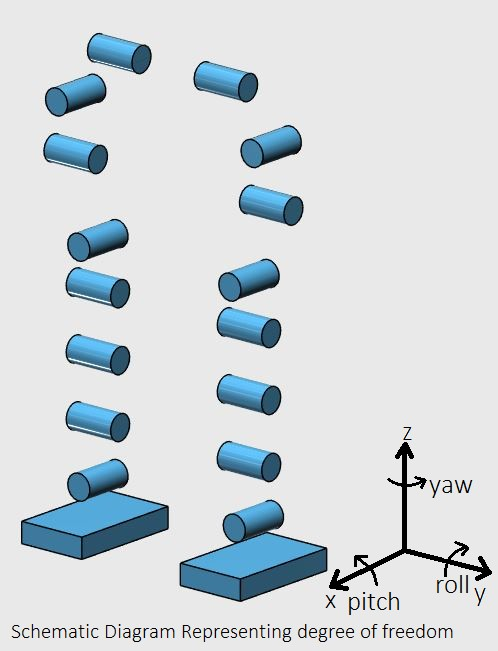
\includegraphics[width=10cm]{Schematic.jpg}\\
\end{center}

The proposed robot has 16 DOFs, with 6 DOFs on upper body and 10
DOFs on lower body. The upper body has 2 arms with
shoulder(2 DOFs each) and elbow (1 DOF each). Lower body has 2
legs with Hip(2 DOFs each), Knee(1 DOF each) and Ankle (2 DOFs each ).


\subsection{Bipedal robots}
Bipedalism is terrestrial locomotion on two limbs. It is the important
means by which human interact with the physical world. Bipedalism enables motion over
rugged surface, allows navigation of complex 3-D routes and frees the arms and hands for
non-locomotory tasks such as object manipulation and gesture communication. Stares,
chairs and ladders and many of the common tools and environmental feature in modern
world is specifically designed for the upright bipedal walkers. Thus crucial for the
humanoid robot to achieve robust bipedal locomotion to preform and function effectively
in the world designed for the bipedal motion of humans.
\\


\subsection{Bipedal motion}
Humans exhibit two principal modes of locomotion

\subsubsection{Walking}
Alternating use of legs with one foot in contact with ground all the time.   Walking by far is the most basic means of transportation in modern world. Human bipedal walking can be characterized with alternating cycles of pendulum and inverted pendulum motions. During a step the leg which is not in contact with ground sweeps forward in pendulum motion. Meanwhile, the leg that makes contact with the ground remains in an extended position while the body vaults over in an inverted pendulum motion, a form of directional falling .Then sweeping leg makes contact with ground while the extended leg leaves the ground and cycle repeats.

\textbf{Characteristics of walking:} In humans, walking is composed of several separate processes which are:
\begin{itemize}
\setlength{\itemsep}{1pt}
\item Vaulting overs a stiff stance leg.
\item Passive ballistic movement of swing leg.
\item A short 'push' from ankle prior to toe-off, propelling the swing leg.
\item Rotation of hips about the axis of the spine, to increase stride length.
\item Rotation of hips about the horizontal axis to improve balancing during stance.

\end{itemize}
	
\subsubsection{Running}
In contrast to walking where one foot is always in contact with ground, the leg are mostly kept straight and center of gravity vaults over the stance legs or legs in inverted pendulum fashion but instead uses rapid leg acceleration to achieve temporary forward ballistic motion. Each stride in running features three phases: the support phase, during which the foot contacts the ground and the leg flexes at knee joint, the drive phase, during which the leg extents at the knee joint, and the recovery phase, during which foot leaves the ground and the hip rotates to drive the leg forward. In addition to motion of legs, significant upper body motion is involved as well to maintain rotational stability.
\newpage
\subsection{Center of mass}
The center of mass of a distribution of mass in space is a unique point where the weighted relative position of the distributed mass sums to zero. The distribution of mass is balanced around the center of mass. In the case of single rigid body, the center of mass is fixed in relation to the body, and if the body has uniform density, it will be located at the centroid. In a uniform gravitational field the center of gravity is identical to center of mass.  The center of gravity (CG) in physics is an imaginary point in a body of matter where, for convenience in certain calculation, the total weight of the body may be thought to be concentrated. The concept is useful in designing static structure or predicting the behavior of moving body when it is acted on by gravity. The center of gravity is an important parameter which is to be determined for the motion of the humanoid robot.\\

whenever an axis of symmetry exists in a structure or a rigid body the center of gravity exists along the line of symmetry.  
\\


\begin{figure}[h]
	\centering
	\subfloat{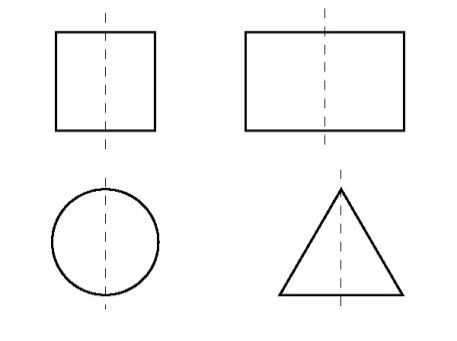
\includegraphics[width = 3in,height= 3 in]{cg1.jpg}} 
	\hspace{1cm}
	\subfloat{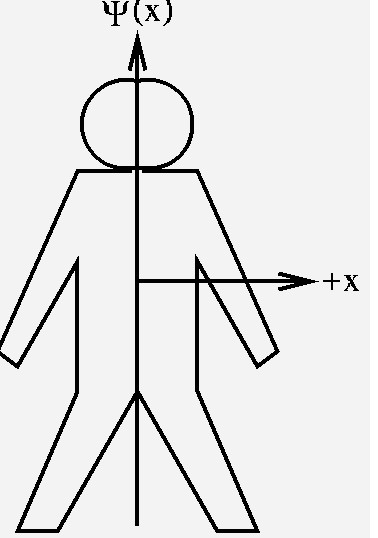
\includegraphics[width = 3in,height= 3 in]{cg2.jpg}}
	\caption{Axis of symmetry}
    \label{fig:Axis of symmetry}
\end{figure}
As shown in the above figure the axis of symmetry is the dotted line and the CG exists
along that line. In case of Figure.\ref{fig:Axis of symmetry} the axis of symmetry is the vertical line passing along the
body and CG exists along that line. Once the line of symmetry is determined the center of
gravity can be found, for a single rigid body the center of gravity will act at the centroid
and centroid for standard shapes can be determined with standard formula. For the
distributed mass the center of gravity can be calculated using below equation:
\begin{equation}
\centering
	X_{com}M = \sum{m_{i} x_{i}} 
	\label{equ: Com}
\end{equation}
 
where,\\
$Xcom$ is the distance of center of mass/center of gravity for the reference point. Figure.\ref{fig:Sch_bot} \\
$M$ is total mass of the system.\\
$m_{i}$ is mass at the distance xi from the reference point.\\
$x_{i}$ is total number of distributed mass.
\newpage
\begin{figure}[h]
	\centering
	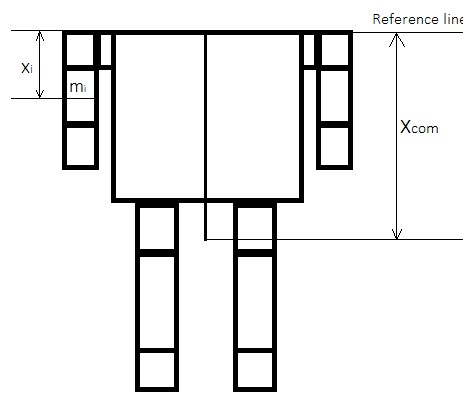
\includegraphics[width=0.4\linewidth, height=7cm]{Sch_bot.jpg} 
	\caption{schematic of robot}
	\label{fig:Sch_bot}
\end{figure}
\subsubsection{Calculation of CG/COM}
Total mass of the body = $M$ grams.
The table gives Mass of each part of structure and their corresponding distance from the
reference line is as follows:\\

\begin{table}[h!]
\centering
	\begin{tabular}{ |l|c|c| } 
		\hline
		Part & Mass($m_{i}$) g & Distance($x_{i}$) mm \\
			\hline
				Shoulder servo-1 & $m_{1}$ & $x_{1}$ \\
				
				Shoulder servo-2 & $m_{2}$ & $x_{2}$ \\
				Torso & $m_{3}$ & $x_{3}$ \\
				Elbow & $m_{4}$ & $x_{4}$ \\
				Upper hip servo & $m_{5}$ & $x_{5}$ \\
				Lower hip servo & $m_{6}$ & $x_{6}$ \\
				Knee servo & $m_{7}$ & $x_{7}$ \\
				upper Ankle servo & $m_{8}$ & $x_{8}$ \\
				Lower ankle servo & $m_{9}$ & $x_{9}$ \\
		\hline
	
		
	\end{tabular}
	\caption{mass and distance of each part}
	\label{tab1:COM}
\end{table}

Using equation.\eqref{equ: Com} we get the $X_{com}$ as:

$$	X_{com} = \frac{m_{1} x_{1} + m_{2} x_{2} + m_{3} x_{3} + m_{4} x_{4} + m_{5} x_{5} + m_{6} x_{6} + m_{7} x_{7} + m_{8} x_{8} + m_{9} x_{9}} {M} $$

\newpage	
\section{Mechanical Design and Construction}
\subsection{Structure of the robot}
\subsubsection{Phase 1 -  Existing Design}
An existing robot structure was provided and we had to assess
the robot structure and list out the faults in the existing design. After the assessment of
structure many faults were found in the design which are listed below:
\begin{enumerate}
	\setlength{\itemsep}{0pt}
	\item Torso was out of proportion with the legs when compared with the human body. This problem could be resolved by reducing the torso size/length.
	\item Shoulder servo (joint) not in line with the hip servo (joint). Due to this, mass was concentrated away from the body due to which the body would topple easily on little deviation from COM (center of mass).   
	\item The bracket moves rather than the servo which is a big disadvantage when a servo needs to sustain large torque. Since the flap (with internal gear) is made of polymer and the gear on the servo is a metal, whenever a large torque acts on the servo the teeth on internal gear of the flap breaks or gets plastically deformed and the contact between the bracket and the servo is lost.(as  shown in the fig e and f)
	\item Design was not robust due to presence of the L-shaped clamp on the knee servo (as shown in the fig b).This problem was resolved by using a square bracket (as shown in the fig c).
\end{enumerate}
The problems stated in [1] [2] and [4] were resolved by modification on the existing
structure but the major issues as stated in [3] was not possible to resolve on the existing
structure hence we decided not to use the existing robot structure but instead design a
new structure.

	\begin{figure}[h]
		\centering
			\subfloat[fig a]{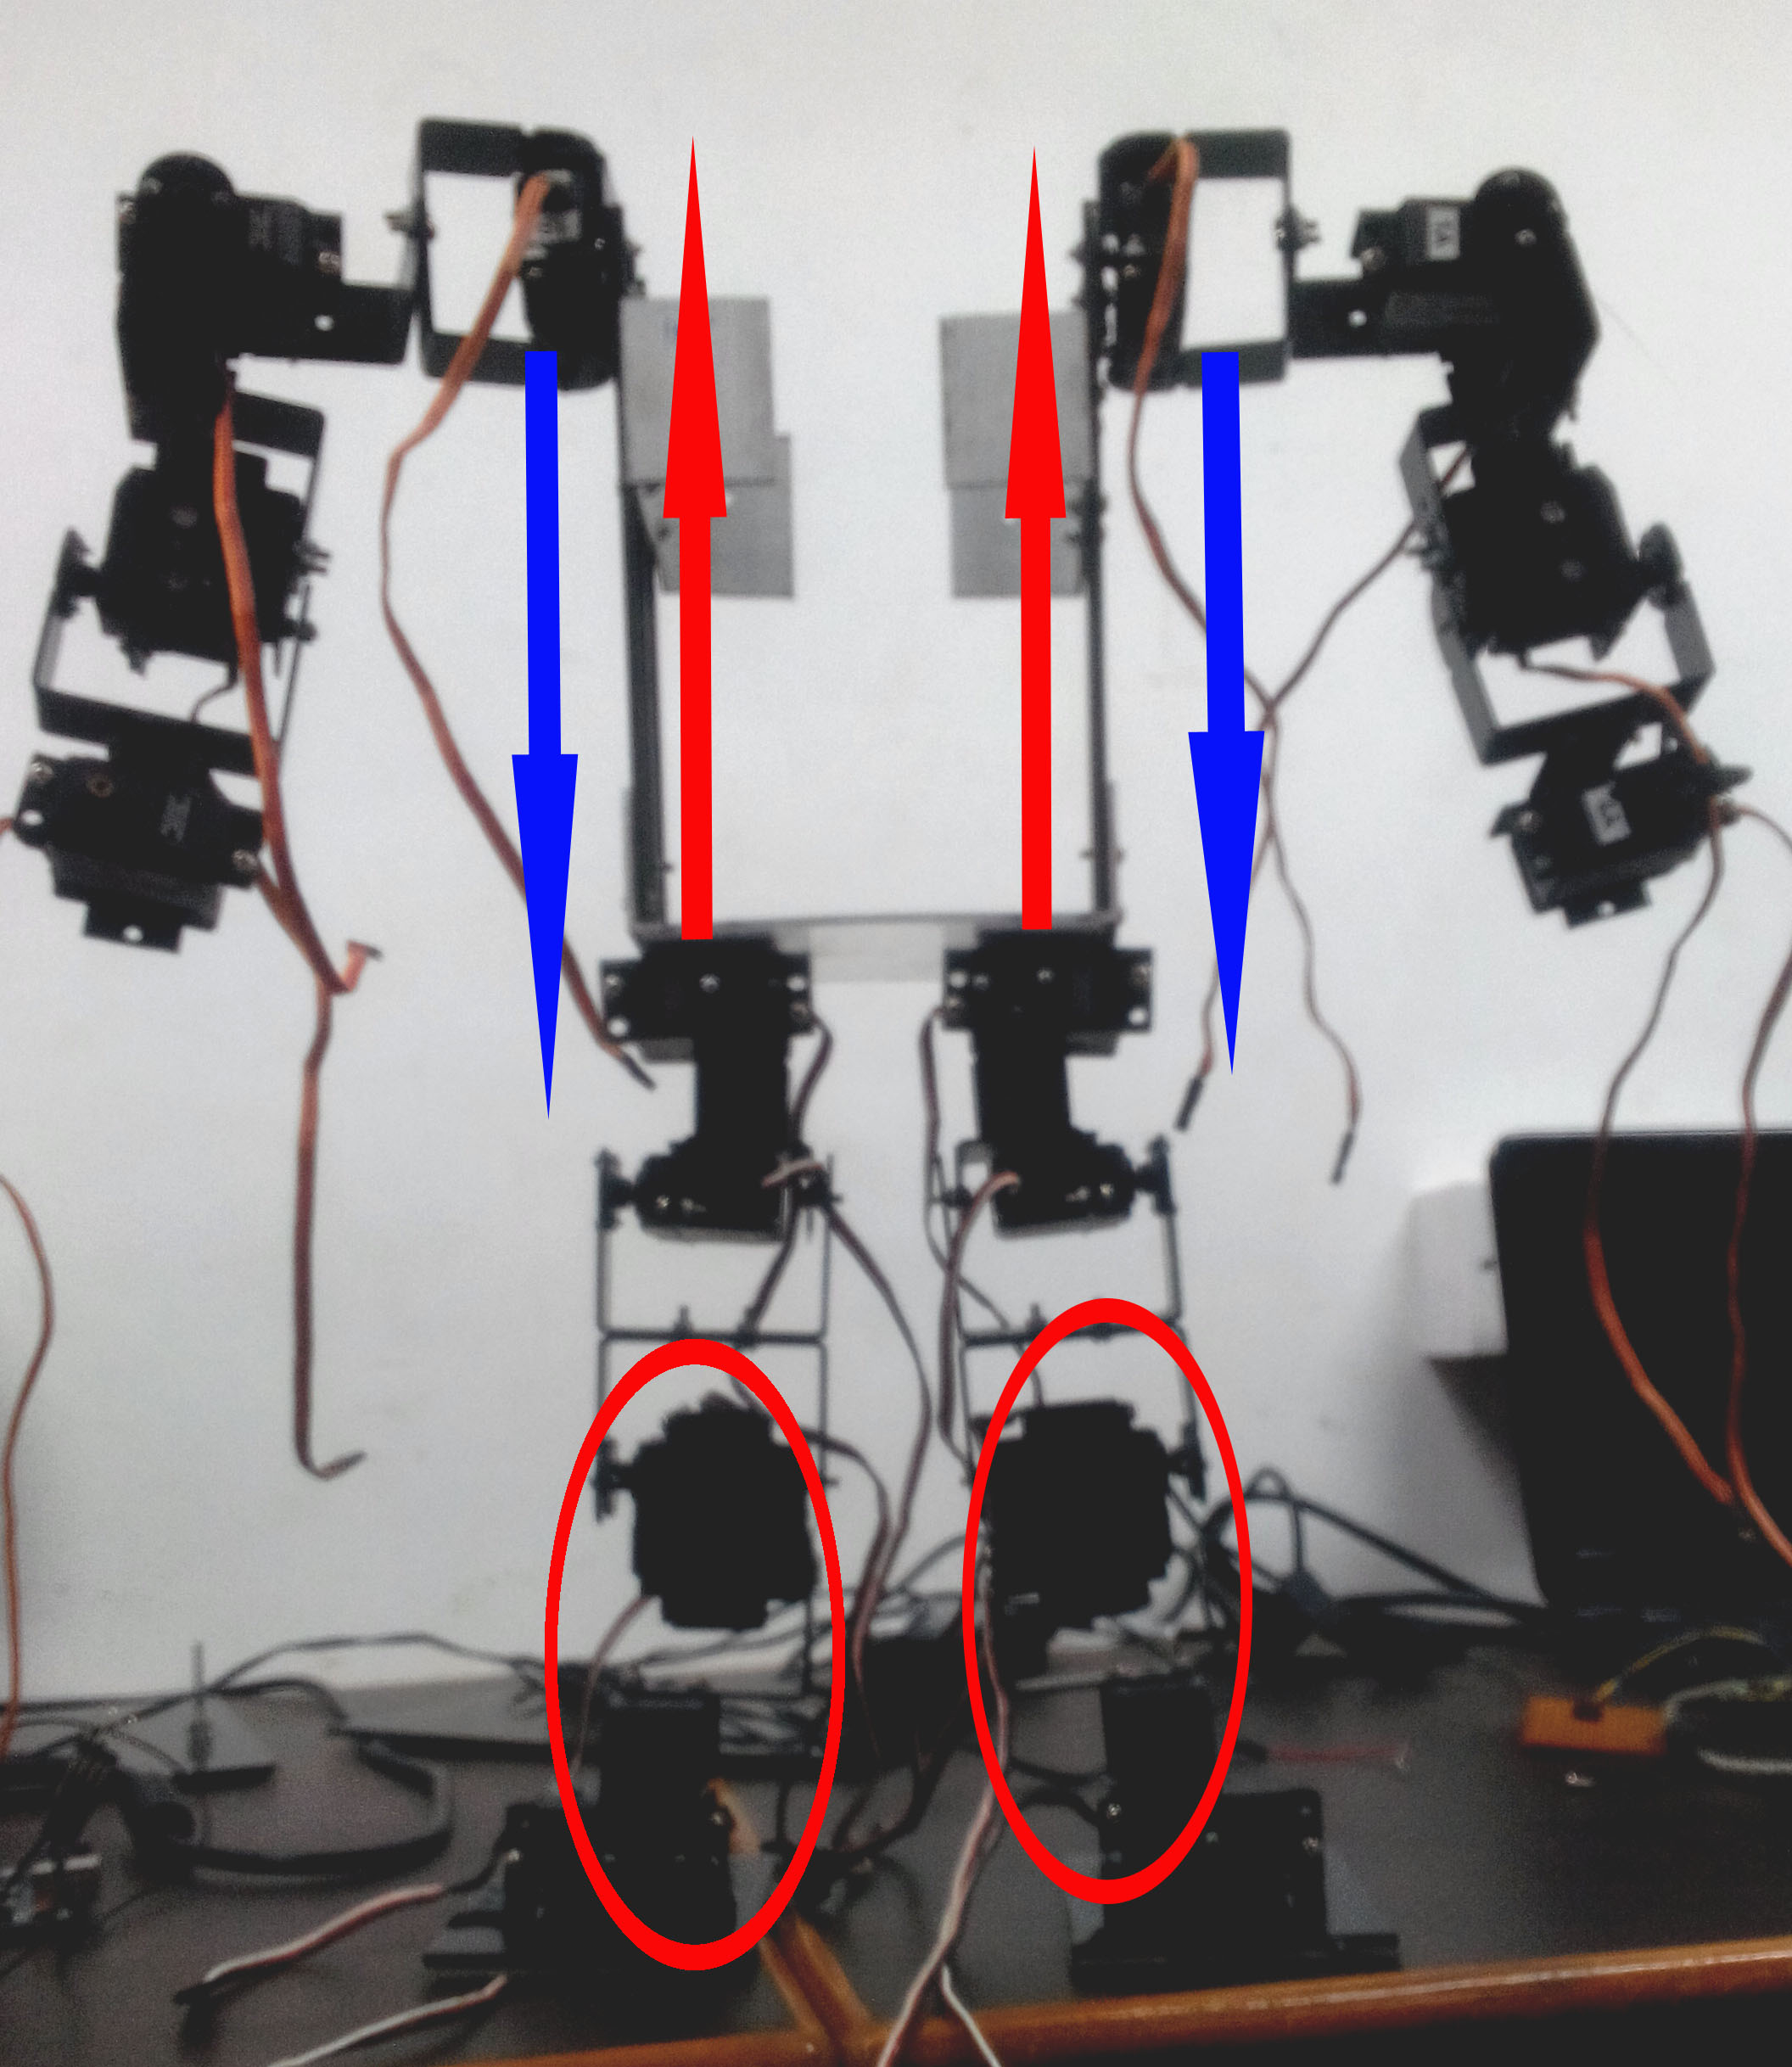
\includegraphics[width = 6cm ,height= 8cm]{Old_bot_highlighted.jpg}} 
			\hspace{2cm}
			\subfloat[fig b]{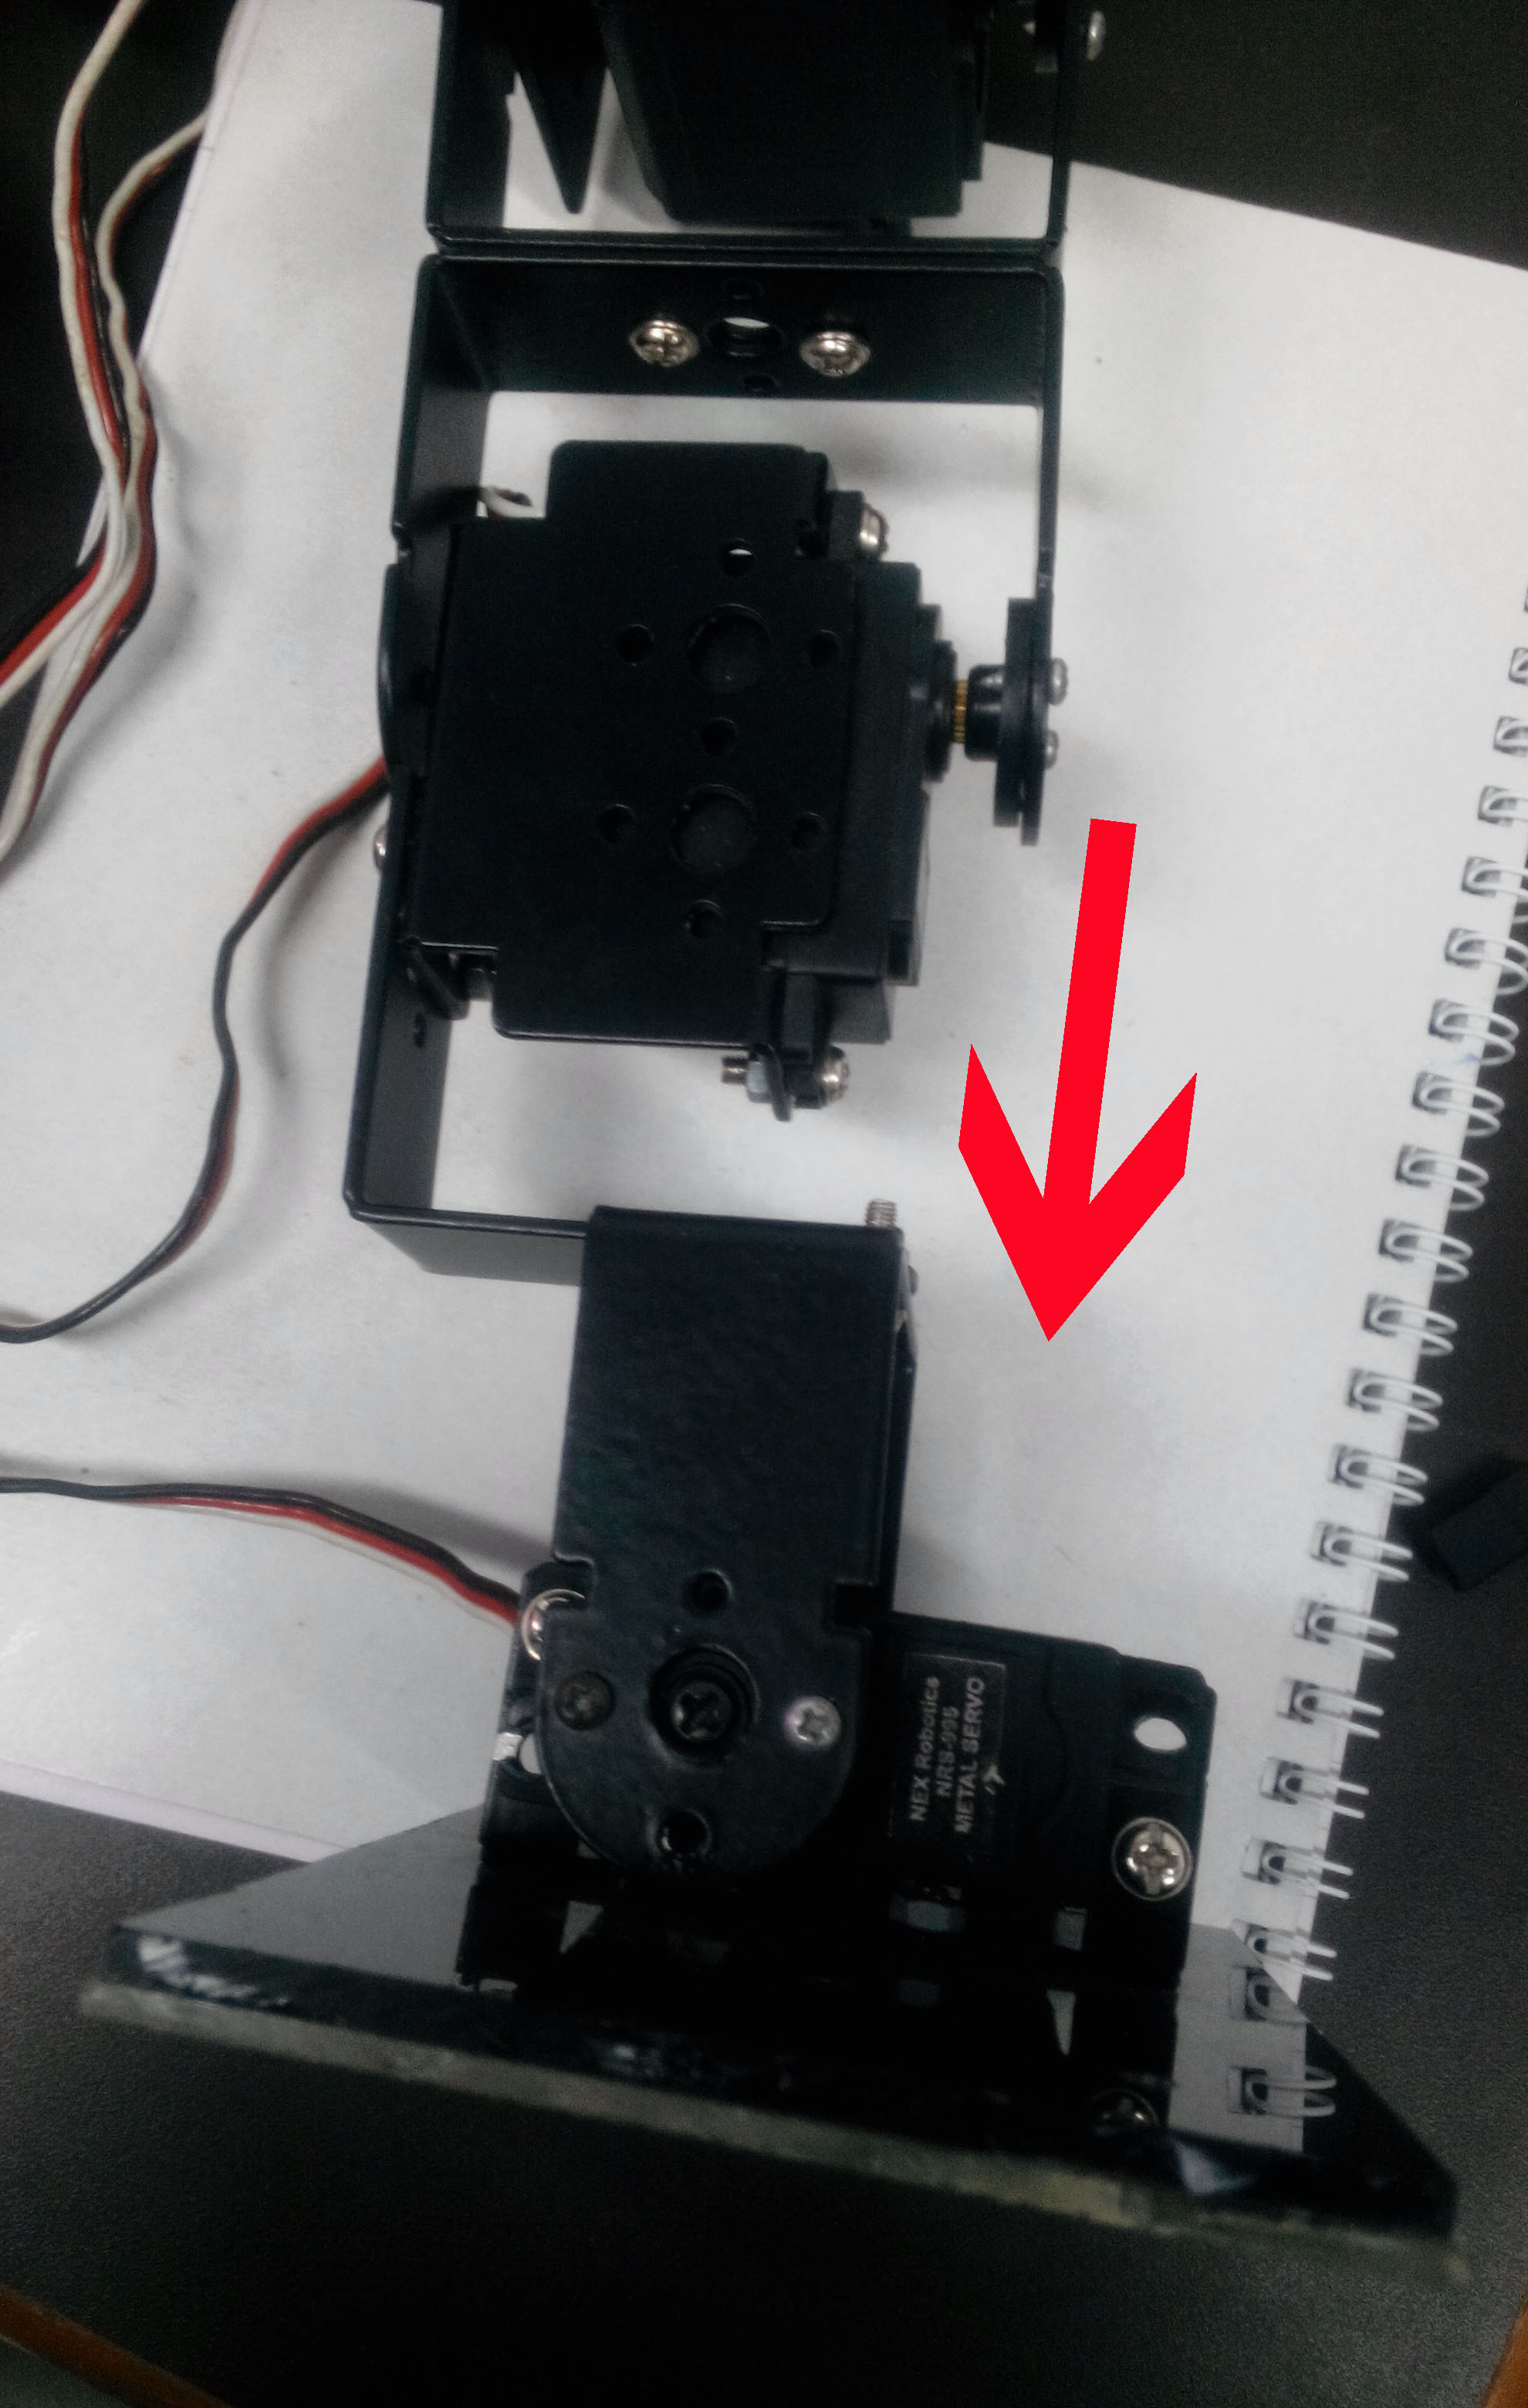
\includegraphics[width = 6cm ,height= 8cm]{magnified_leg_joint_old.jpg}}
	\caption{Mech design phase1}
		\label{fig: Mech design phase1}
		
	\end{figure}
\begin{figure}
	
	
	\ContinuedFloat 
	\centering
	\subfloat[fig c]{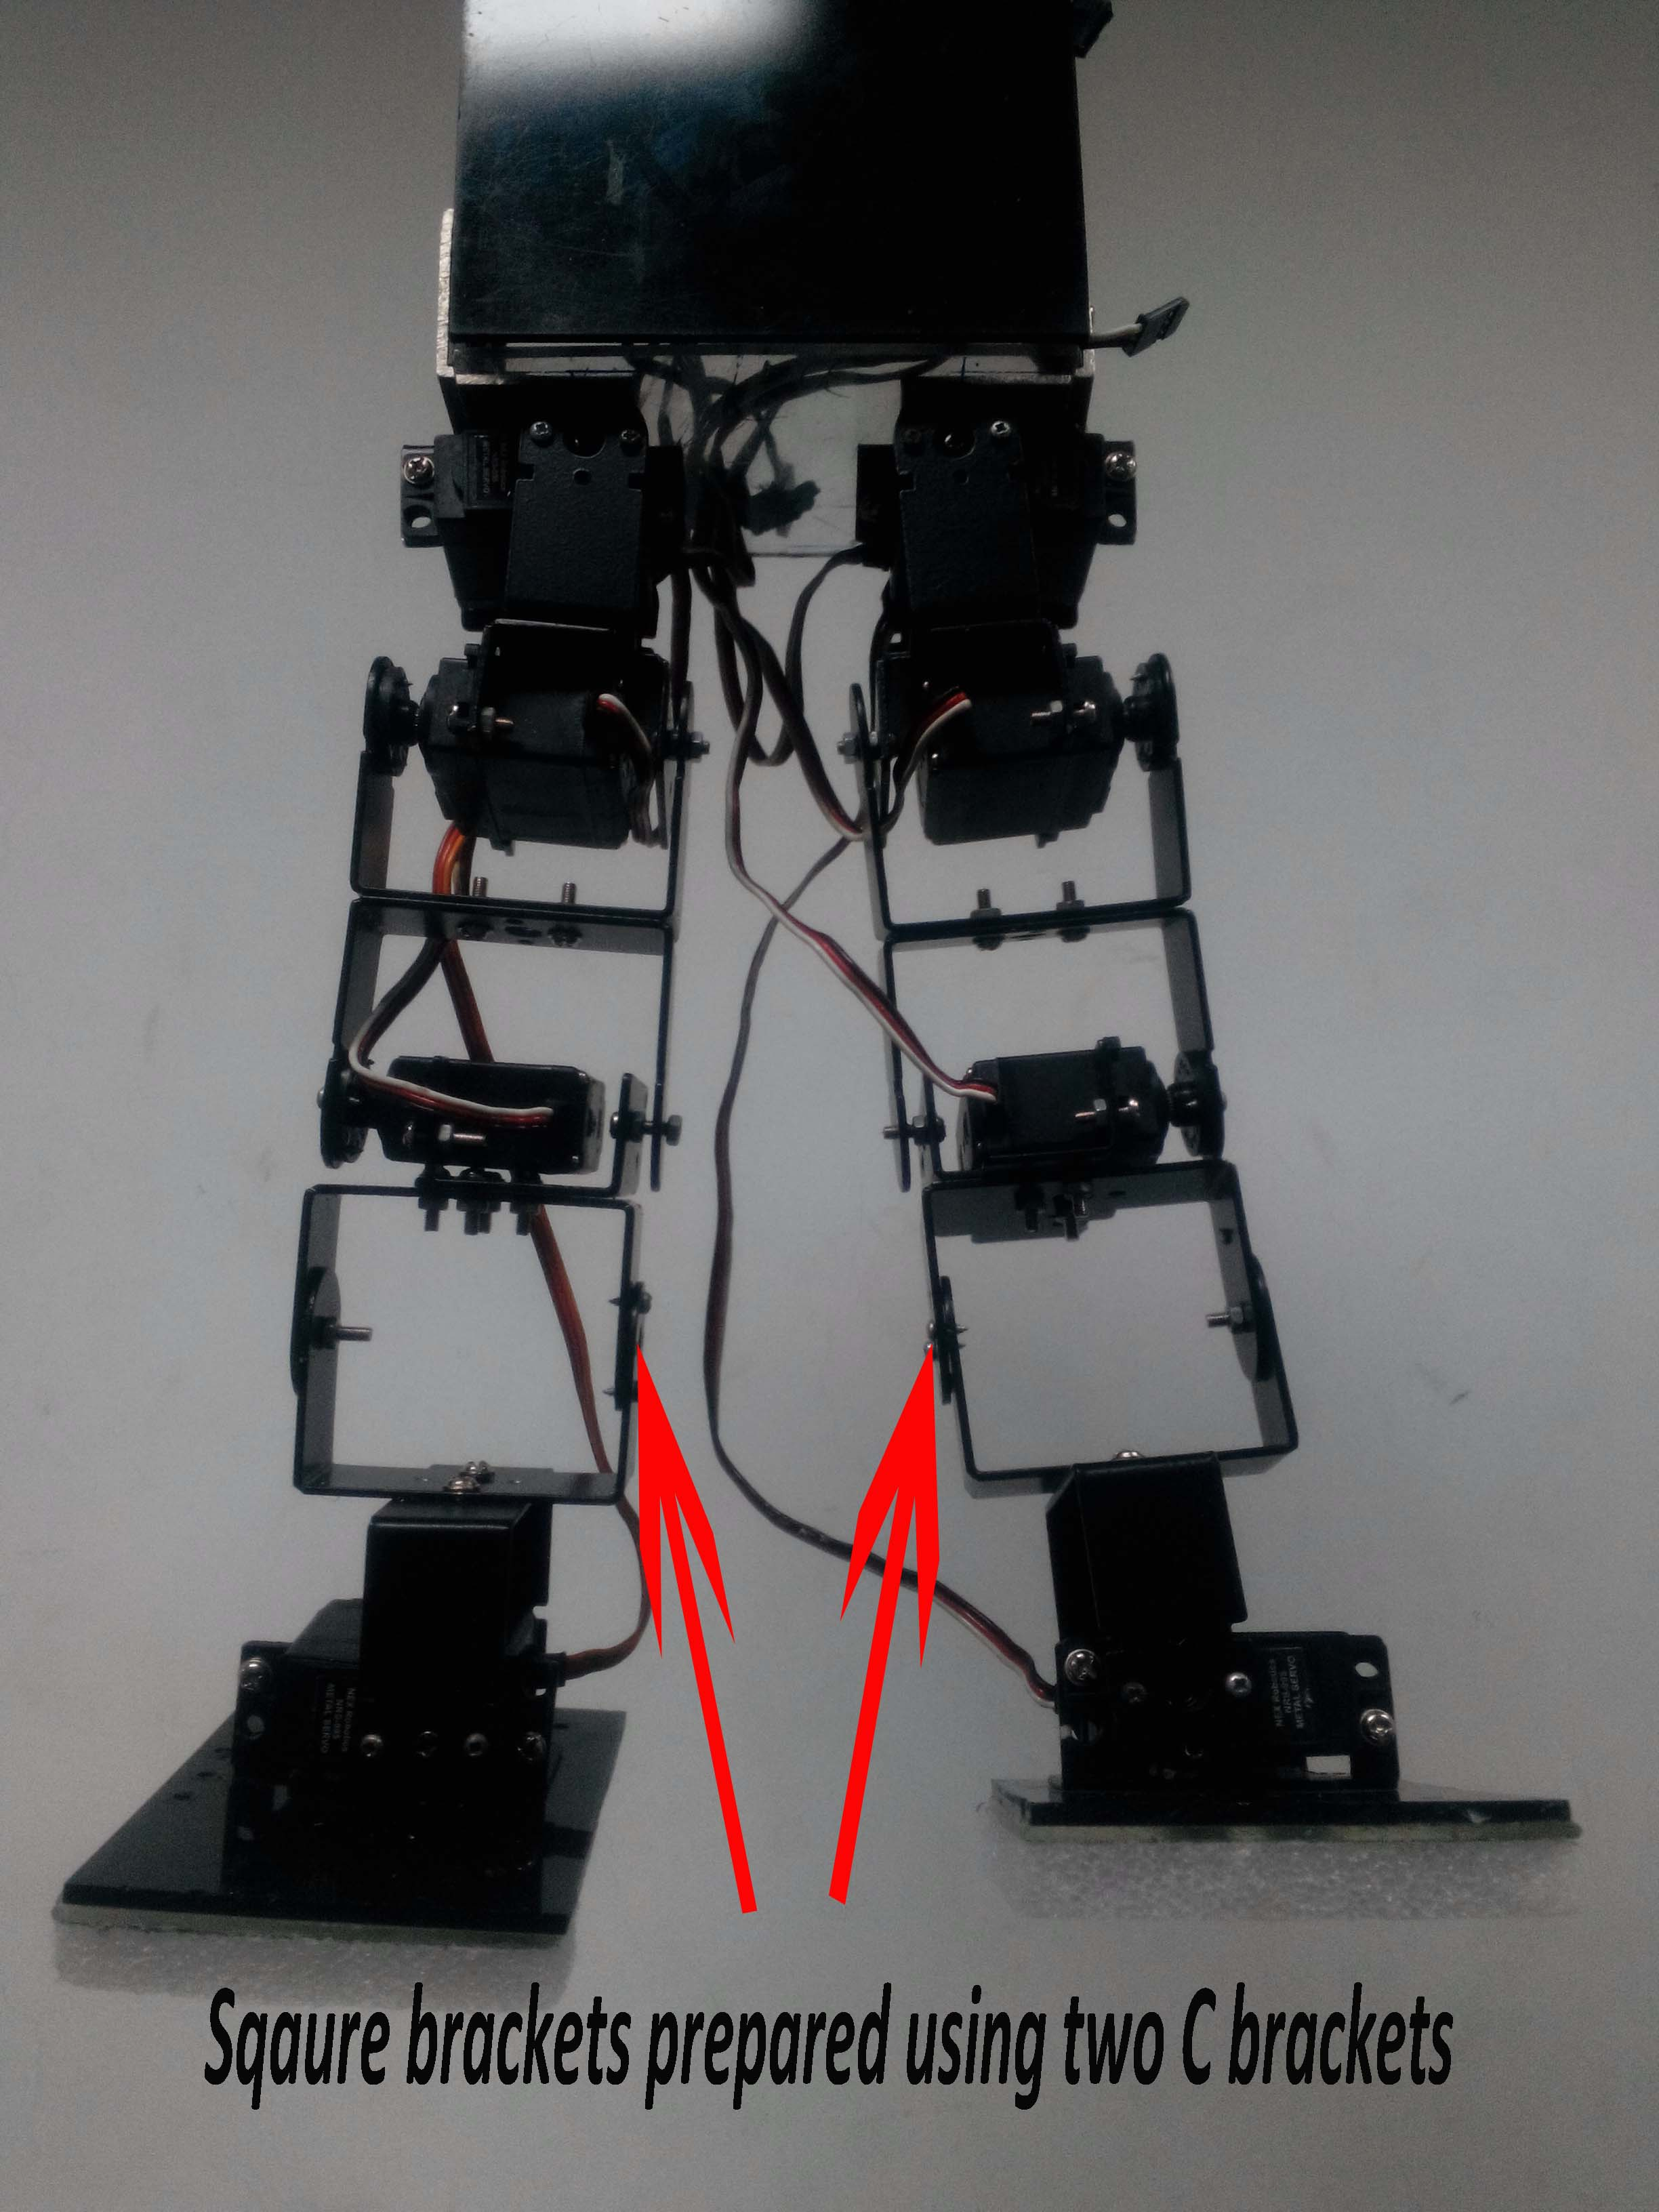
\includegraphics[width = 6cm ,height= 8cm]{square_brackets.jpg}} 
	\hspace{2cm}
	\subfloat[fig d]{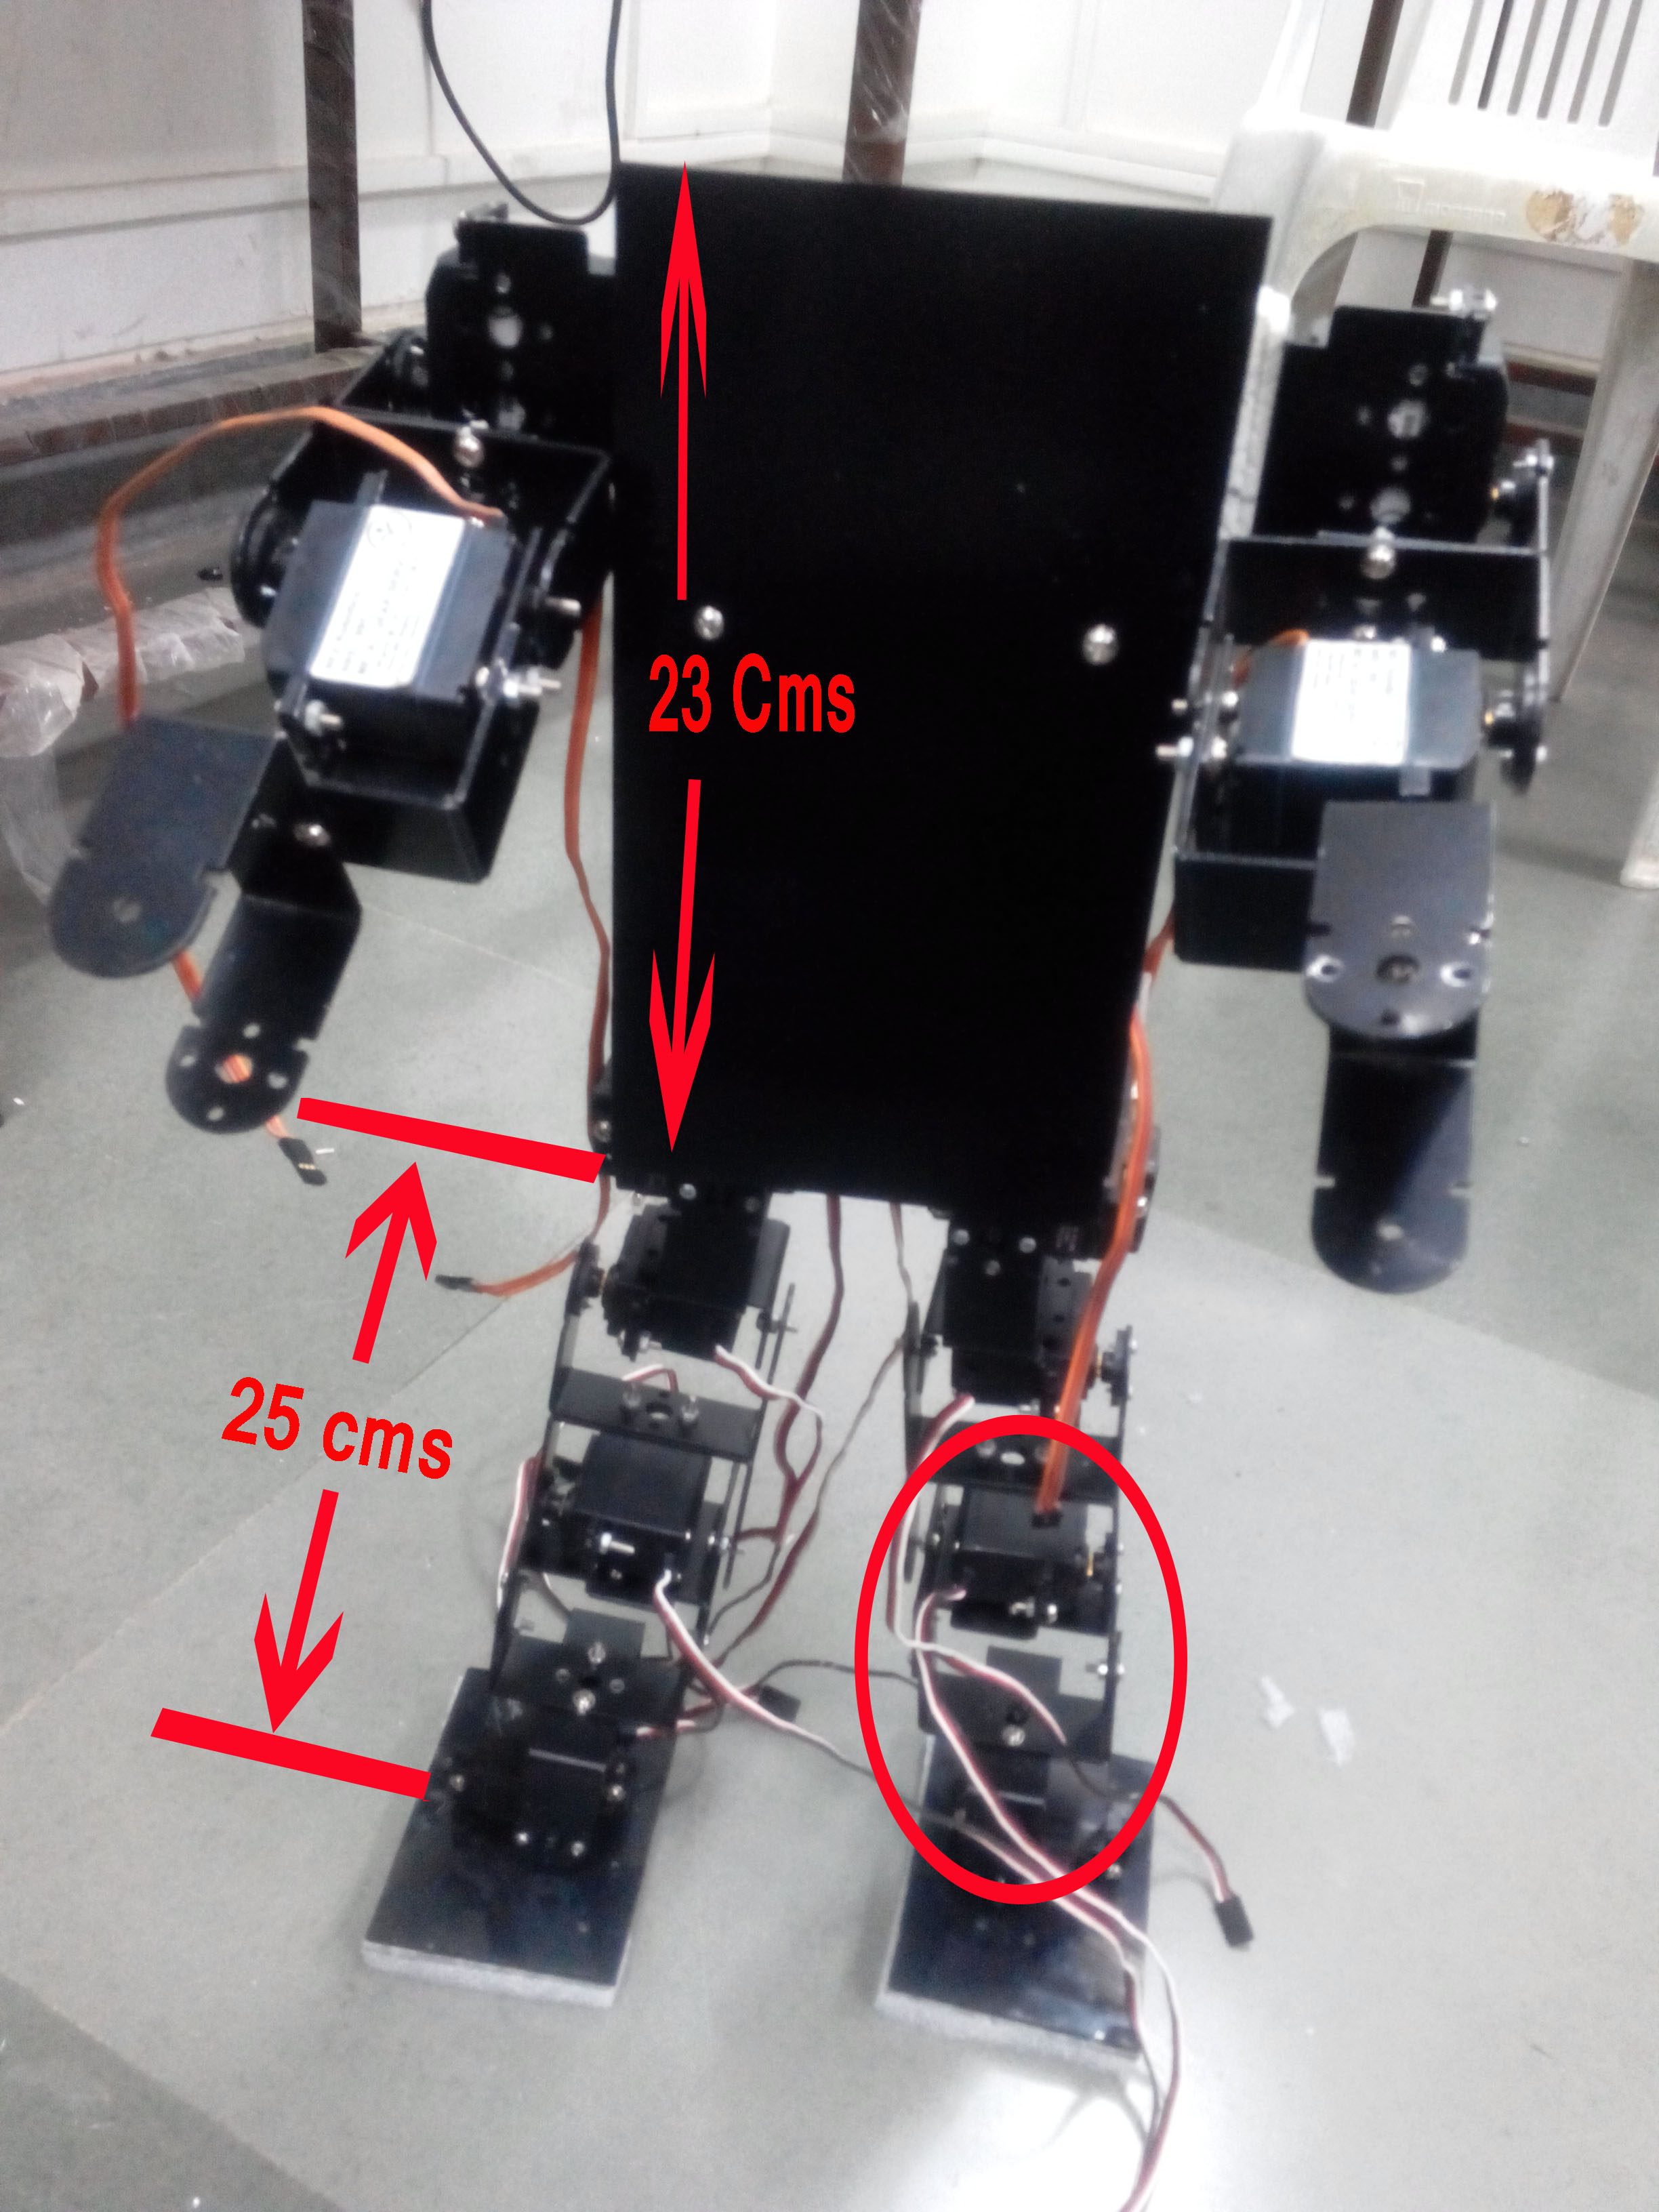
\includegraphics[width = 6cm ,height= 8cm]{torso_proportion.jpg}}
	\newline
	
	\subfloat[fig e]{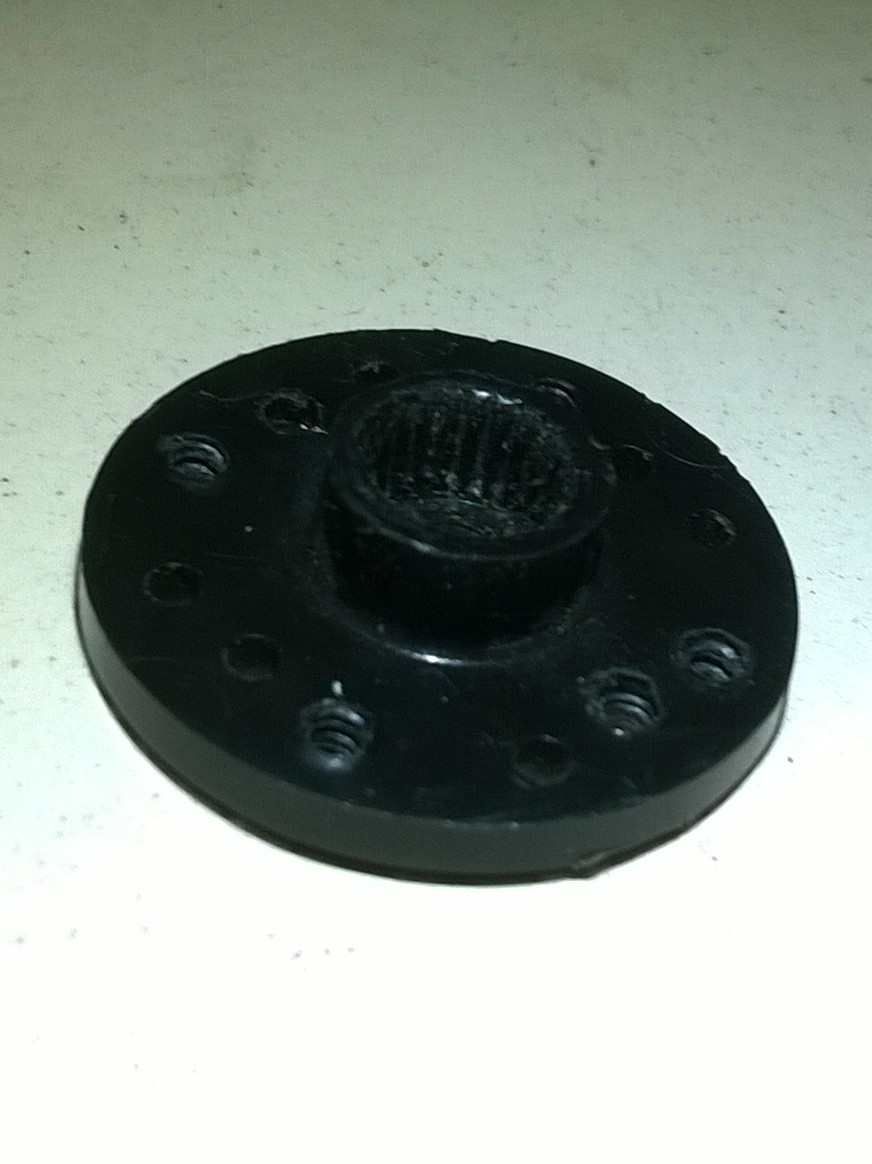
\includegraphics[width = 6cm ,height= 8cm]{WP_20140611_005.jpg}} 
	\hspace{2cm}
	\subfloat[fig f]{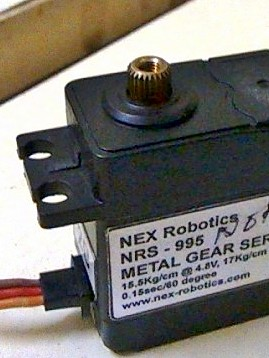
\includegraphics[width = 6cm ,height= 8cm]{WP_20140611_007.jpg}}
	
	\caption{Mech design phase1}
	
	\label{fig: Mech design phase1}
\end{figure}

\newpage

\subsubsection{Phase 2 - New design}
A new structure designed with 14 DOFs with upper body
having 6 DOFs (3 DOFs for each arm) and lower body having 8 DOFs (4 DOFs for
each leg). This structure was designed keeping in mind the faults of previous design,
changes made are listed below
\begin{enumerate}
	\item As the major issue in existing design was the breakage of the teeth in internal
	gear on application of large torque. To resolve this issue we design the structure
	in such a way that the servo would move, keeping the bracket fixed, the
	advantage of this method was that whenever a lager torque is applied the gears
	present inside the servo would move, keeping the flap (internal gear) and the gear
	attached to it constant and the gear present inside the servo are made up of same
	material and strong to sustain that high torque (as shown in Fig c).
	\item The torso and the leg length were in proportion in comparison to human body.
	\item The shoulder servo and the hip servo were in line (shown in Fig a).
	\item The new structure was robust compared to the old design.
\end{enumerate}

\begin{figure}[h]
	\centering
	\subfloat[fig a]{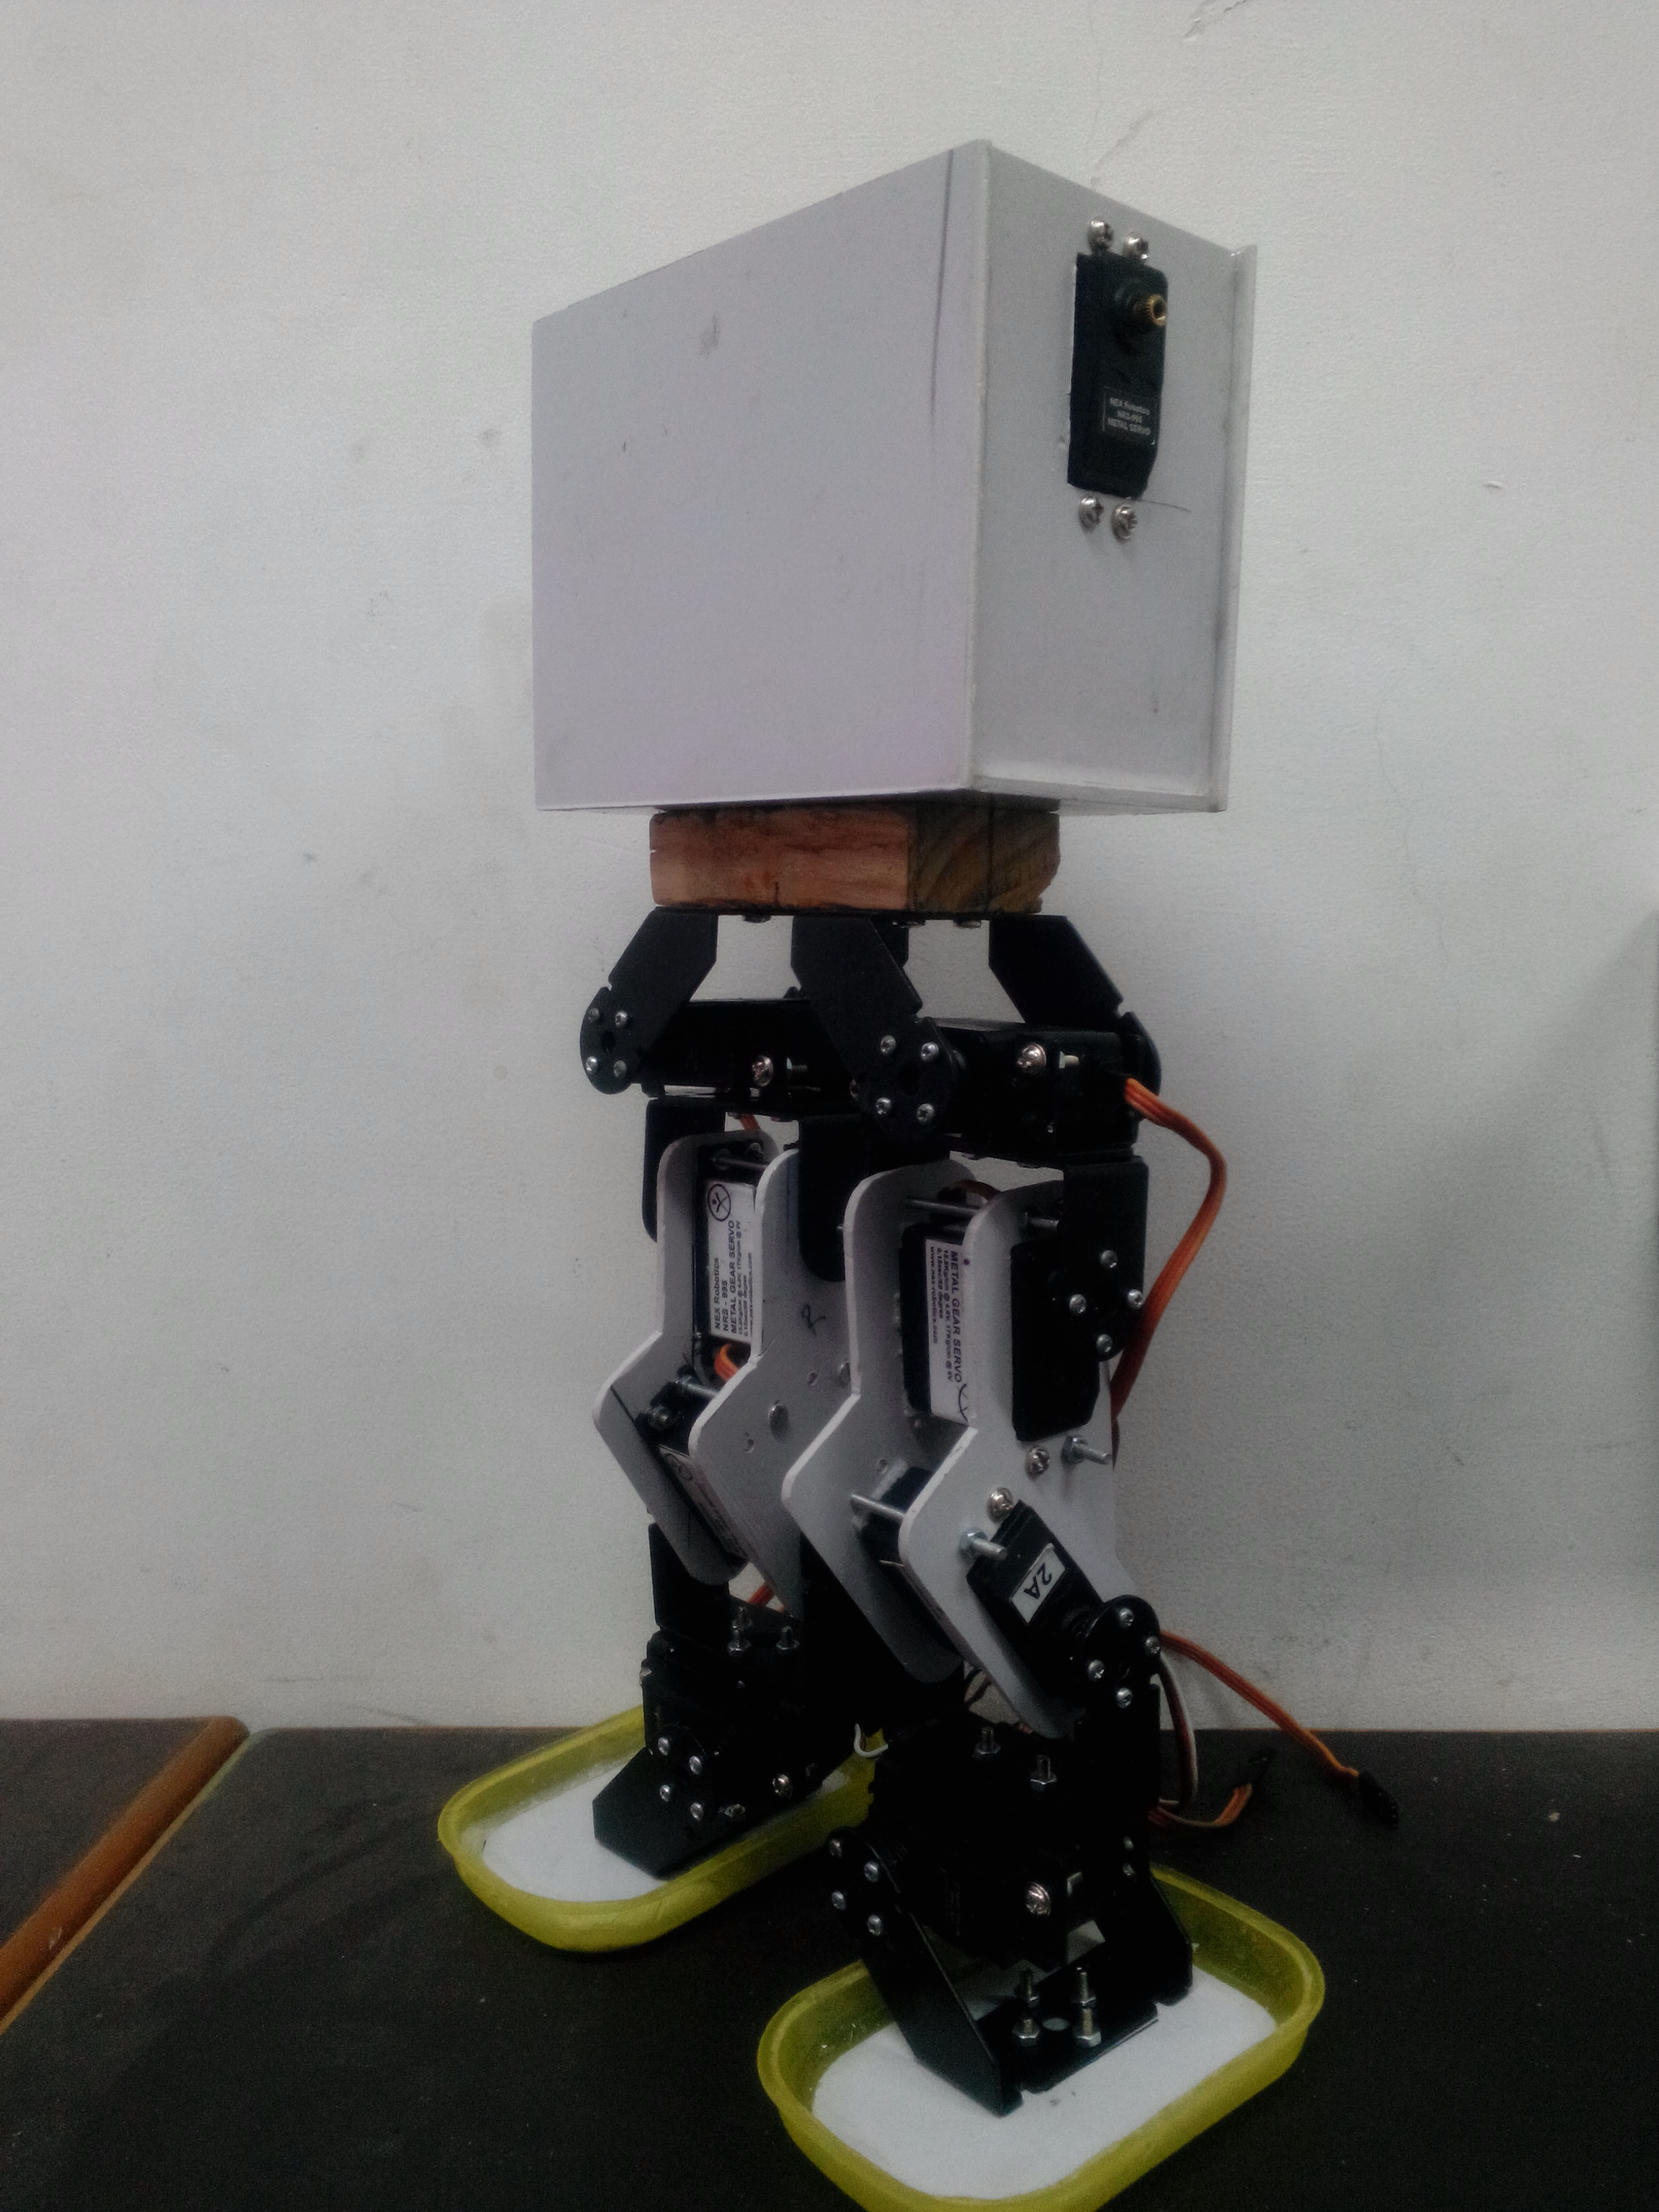
\includegraphics[width = 6cm,height= 7cm]{IMG_20140607_114231.jpg}} 
	\hspace{2cm}
	\subfloat[fig b]{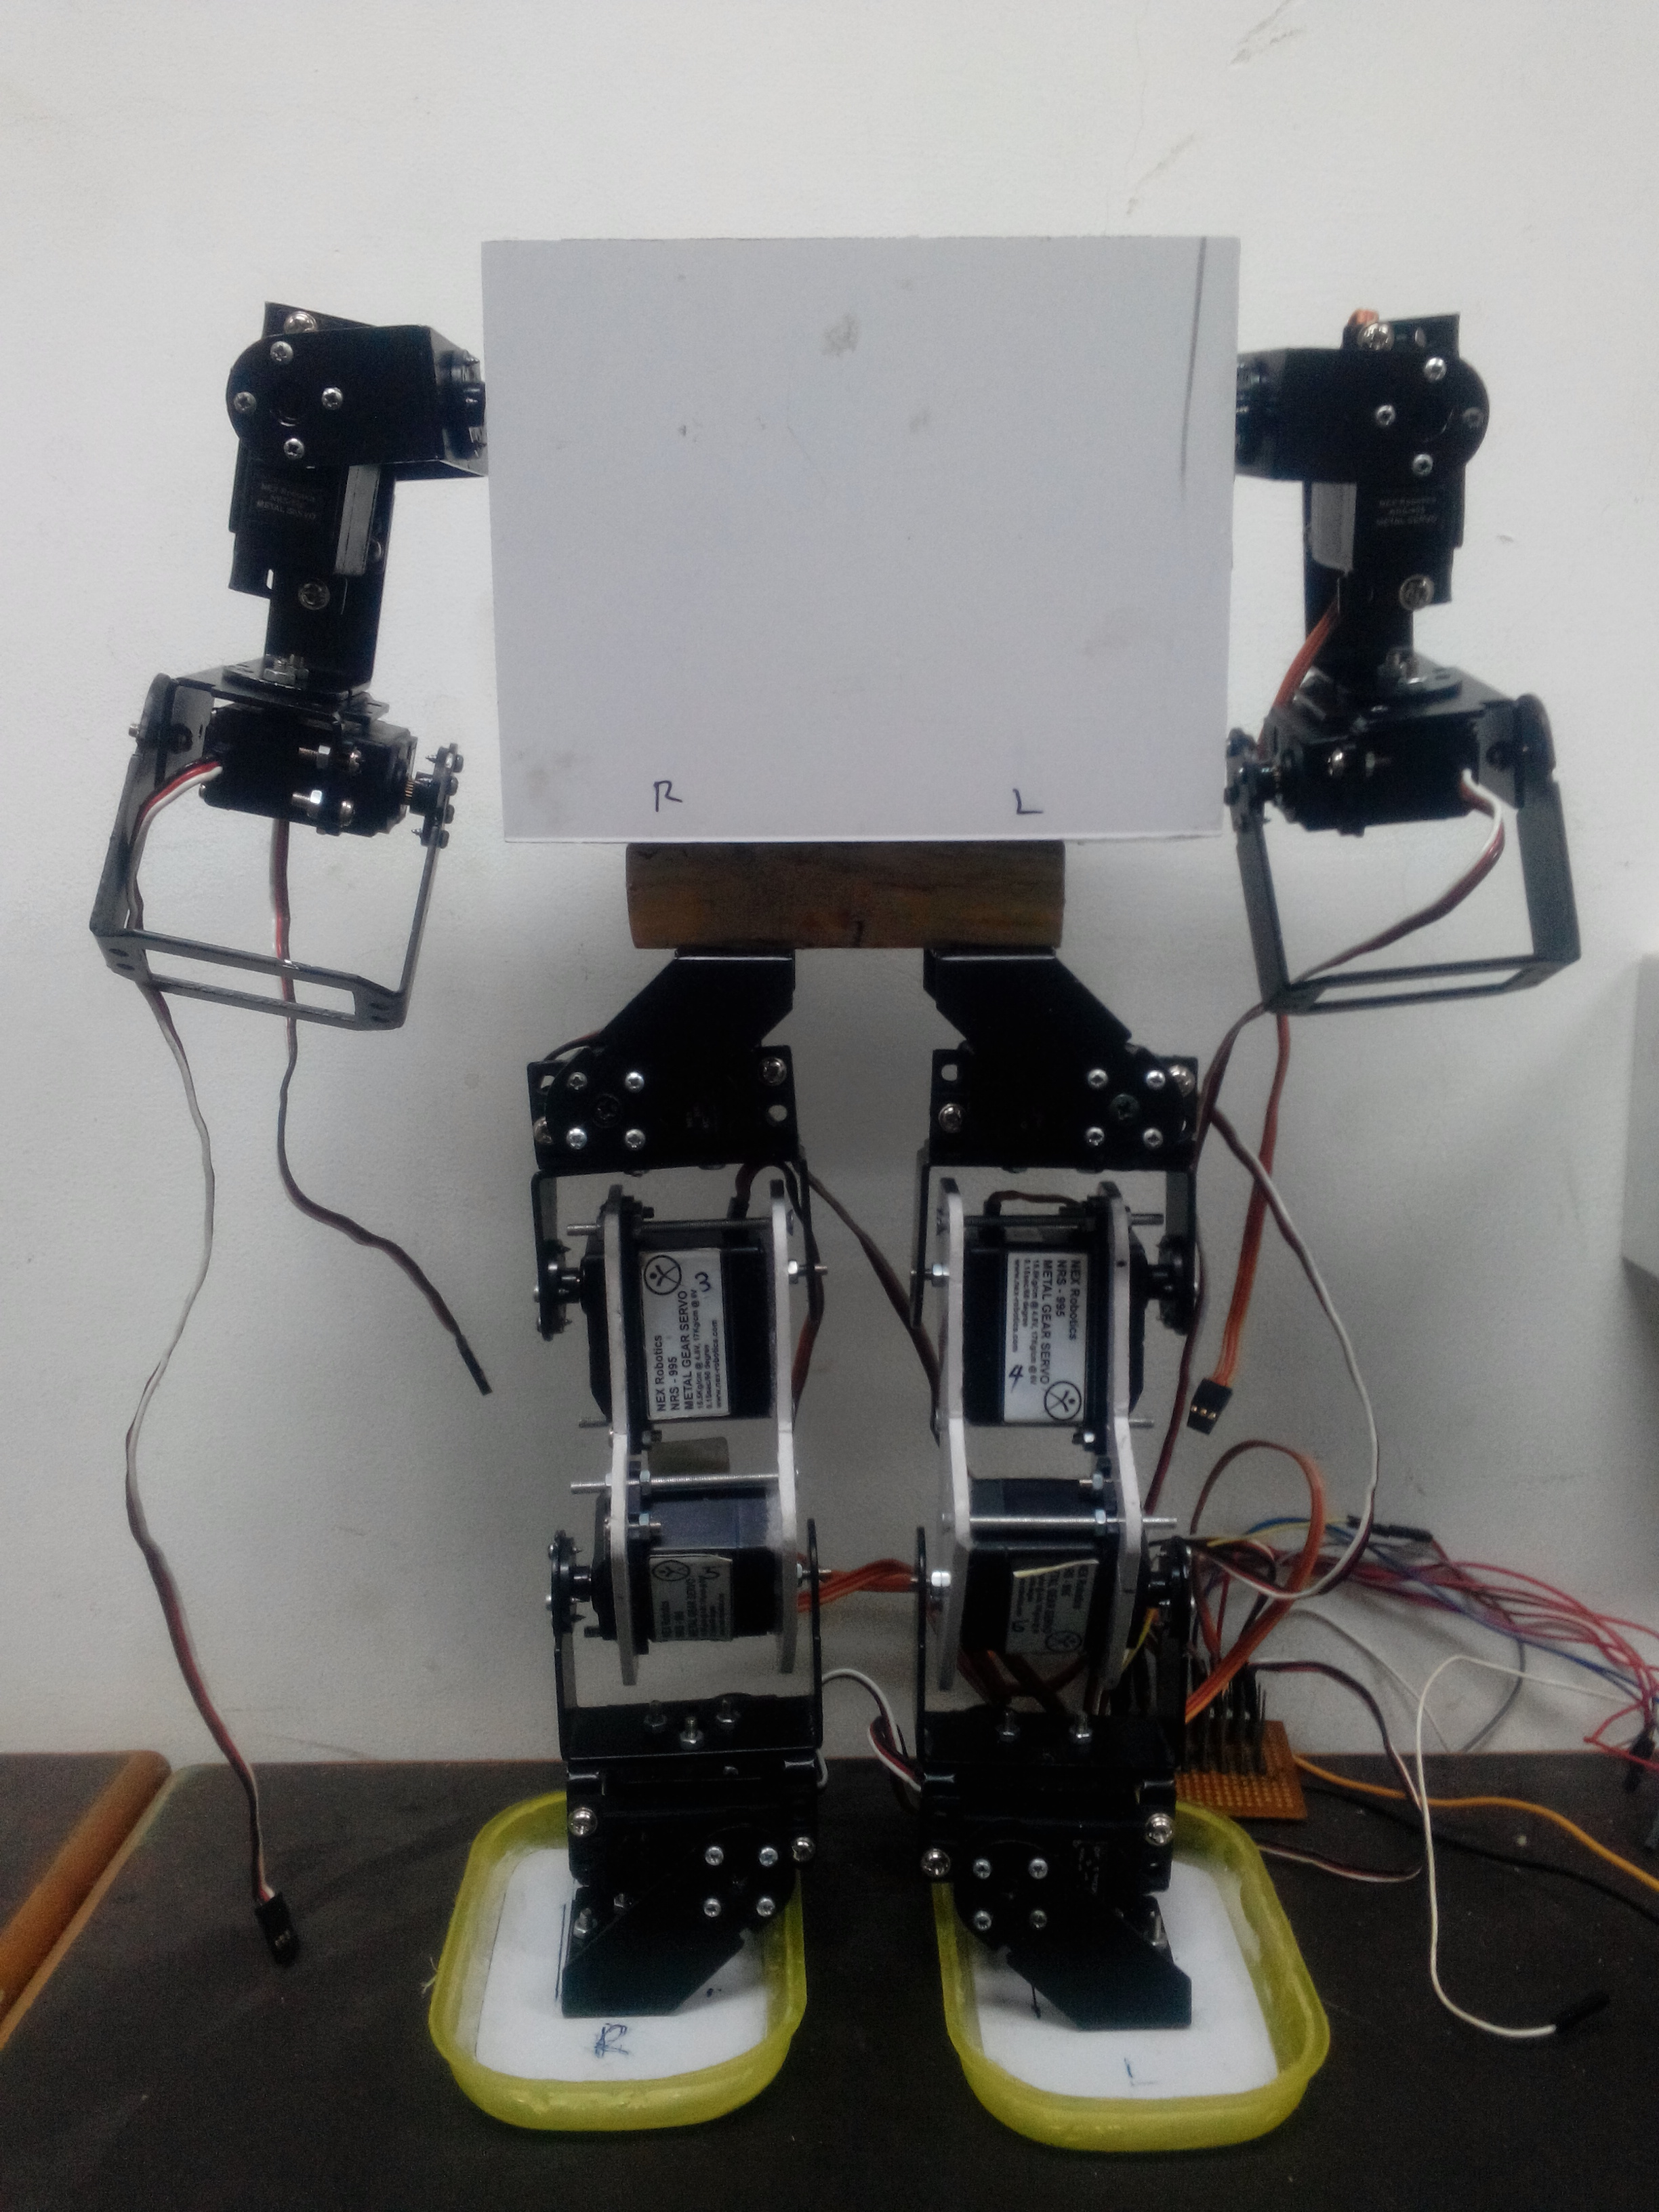
\includegraphics[width = 6cm,height= 7cm]{IMG_20140607_214454.jpg}}
	\newline
	\subfloat[fig c]{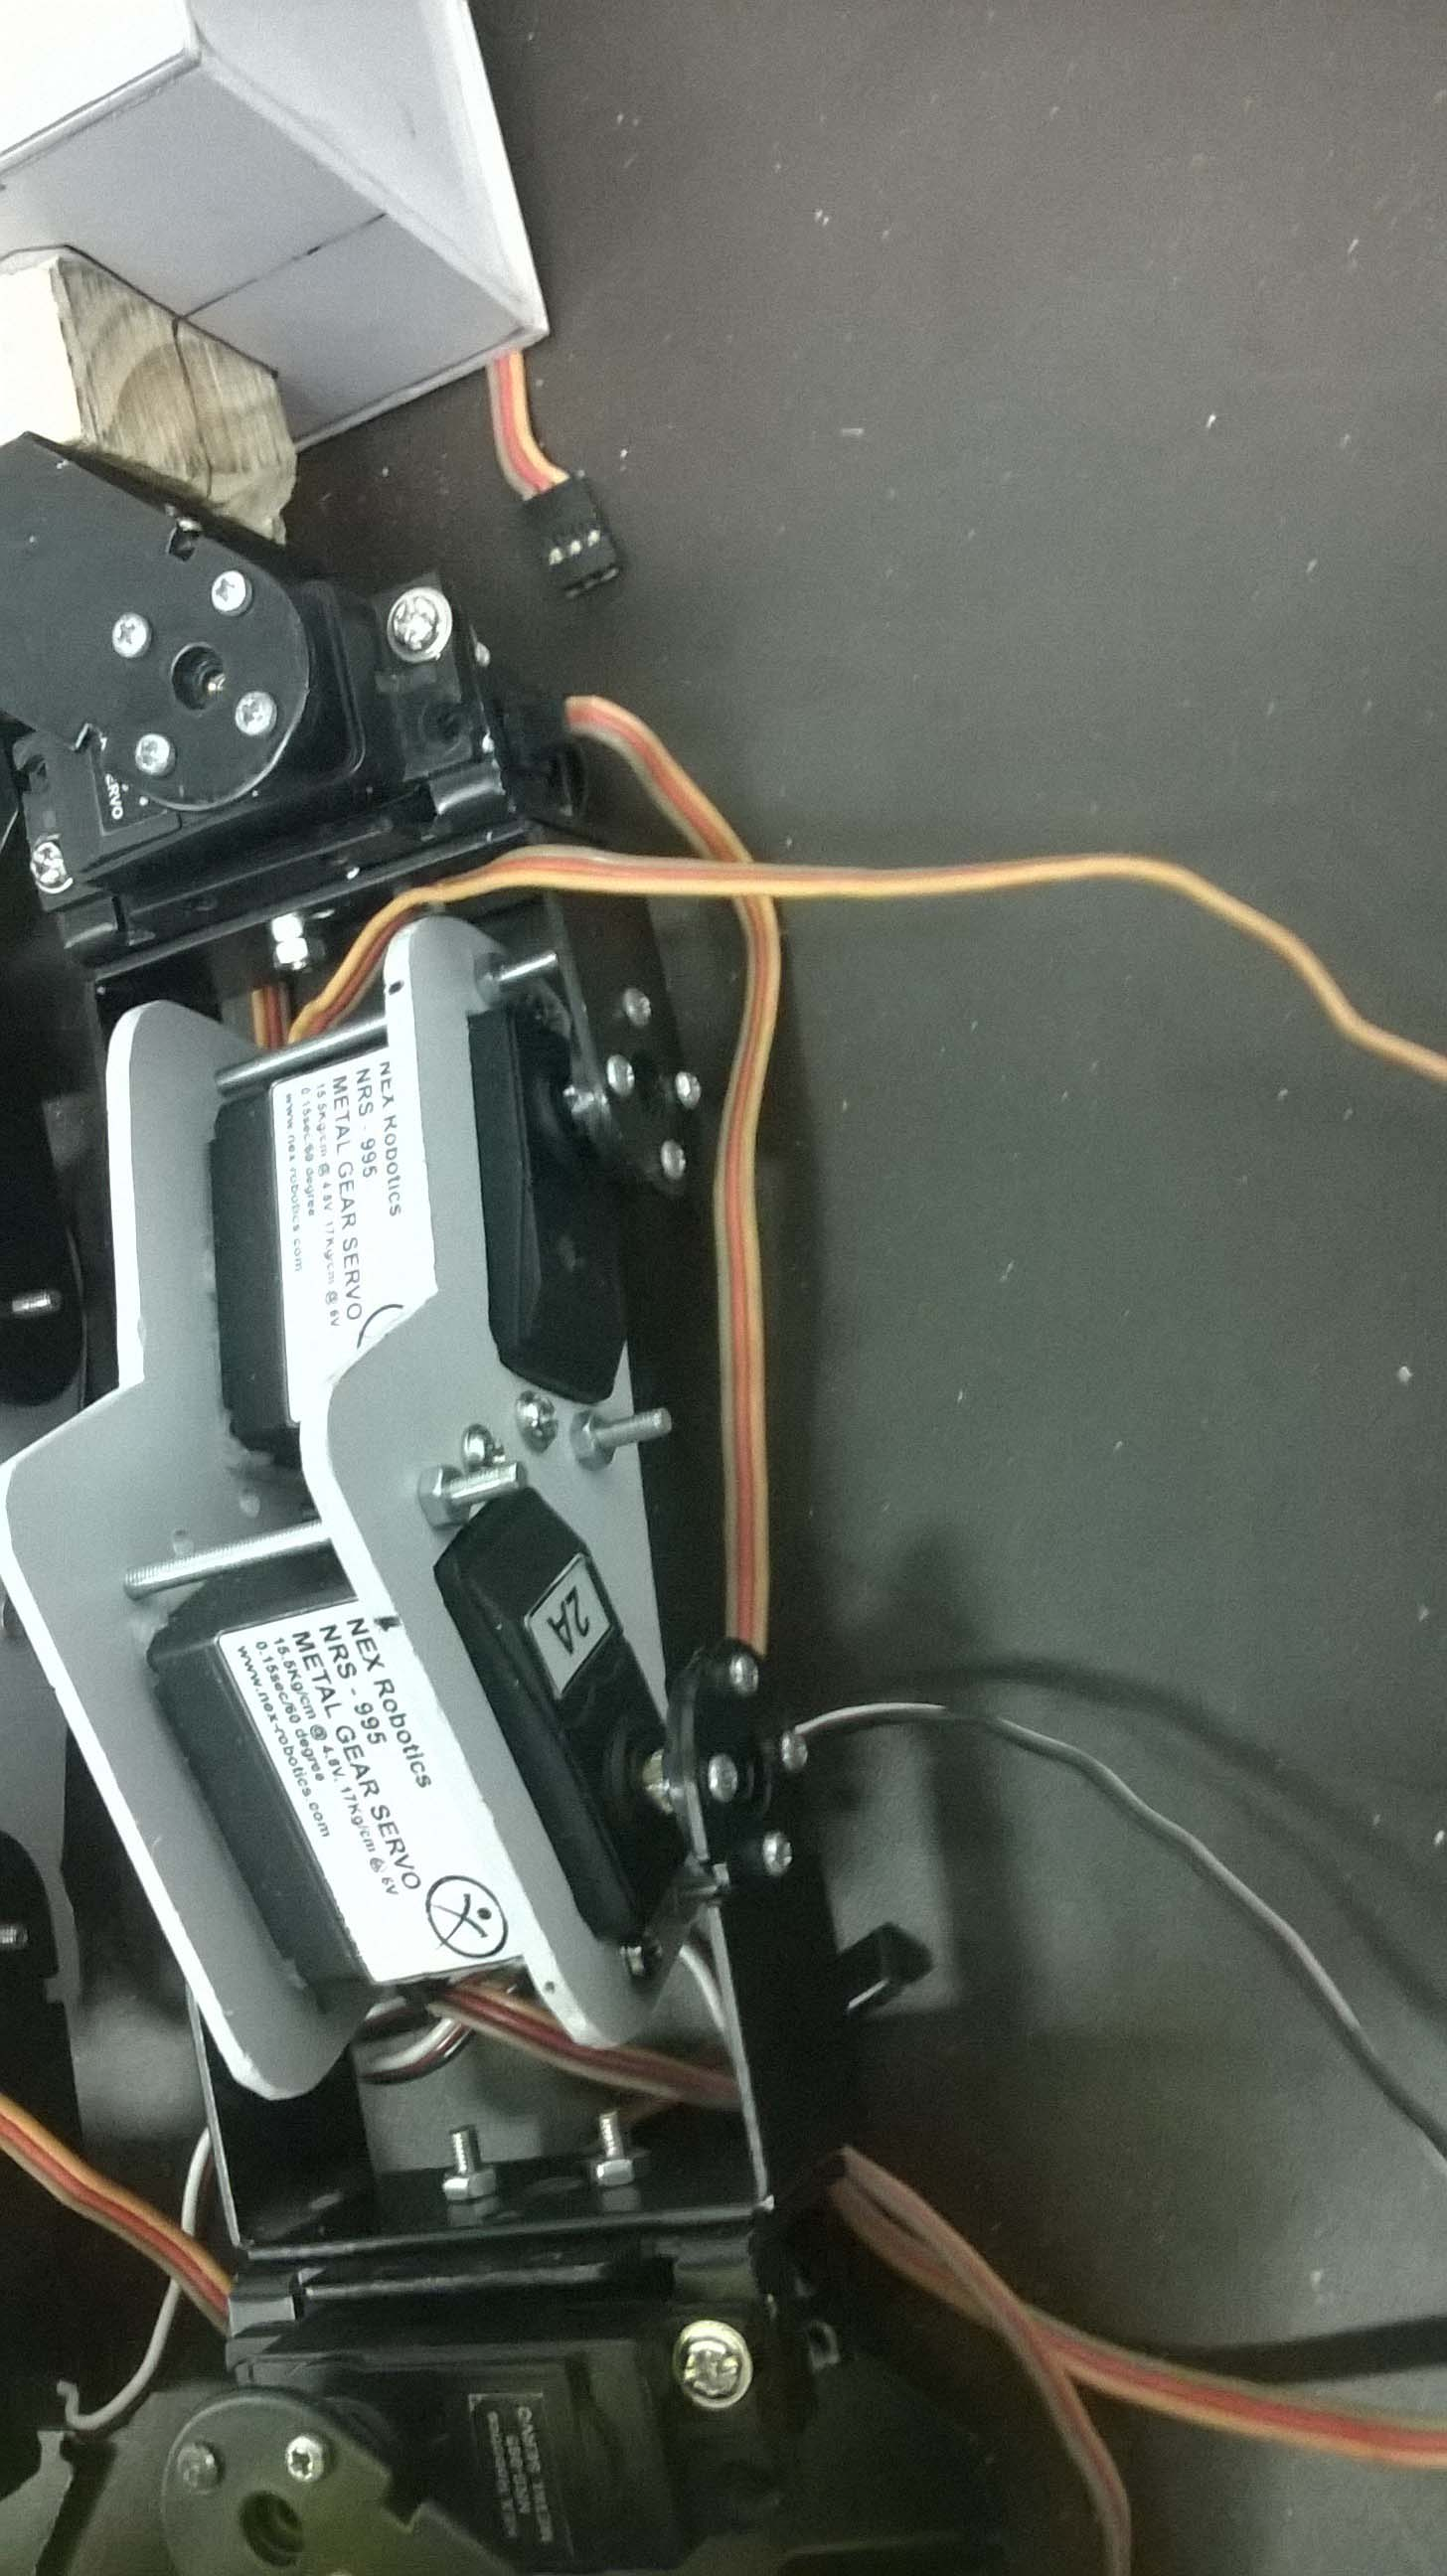
\includegraphics[width = 6cm,height= 7cm]{hip.jpg}}
	
	
	\label{fig:phase2design}
\end{figure}

\subsubsection{Phase 3 – Modifications in New Design}
The basic logic of walking was applied to the new design and algorithm was written but
the outcome was unacceptable due absence of an additional ankle servo during the stage
where the raised foot was brought down by the lower hip and knee servo of the other leg
the whole the robot bends down. Foot is not always parallel to the ground due to which the
front portion of the foot during rising of leg would be dragged against the ground making
the robot walk in an awkward unrealistic way.\\
So to tackle this problem an additional ankle servo was added for each leg which resulted
in 16 DOFs final design. With help of that one servo and the bot remain upright. This
facilitated the motion of the robot close to human like walk.

\subsection{Construction of Robot}
The detailed construction of the final design is explained below.\\
List of all the components with Images:
\begin{figure}[h]
	\centering
	\subfloat[High torque Metal Gear Servo]{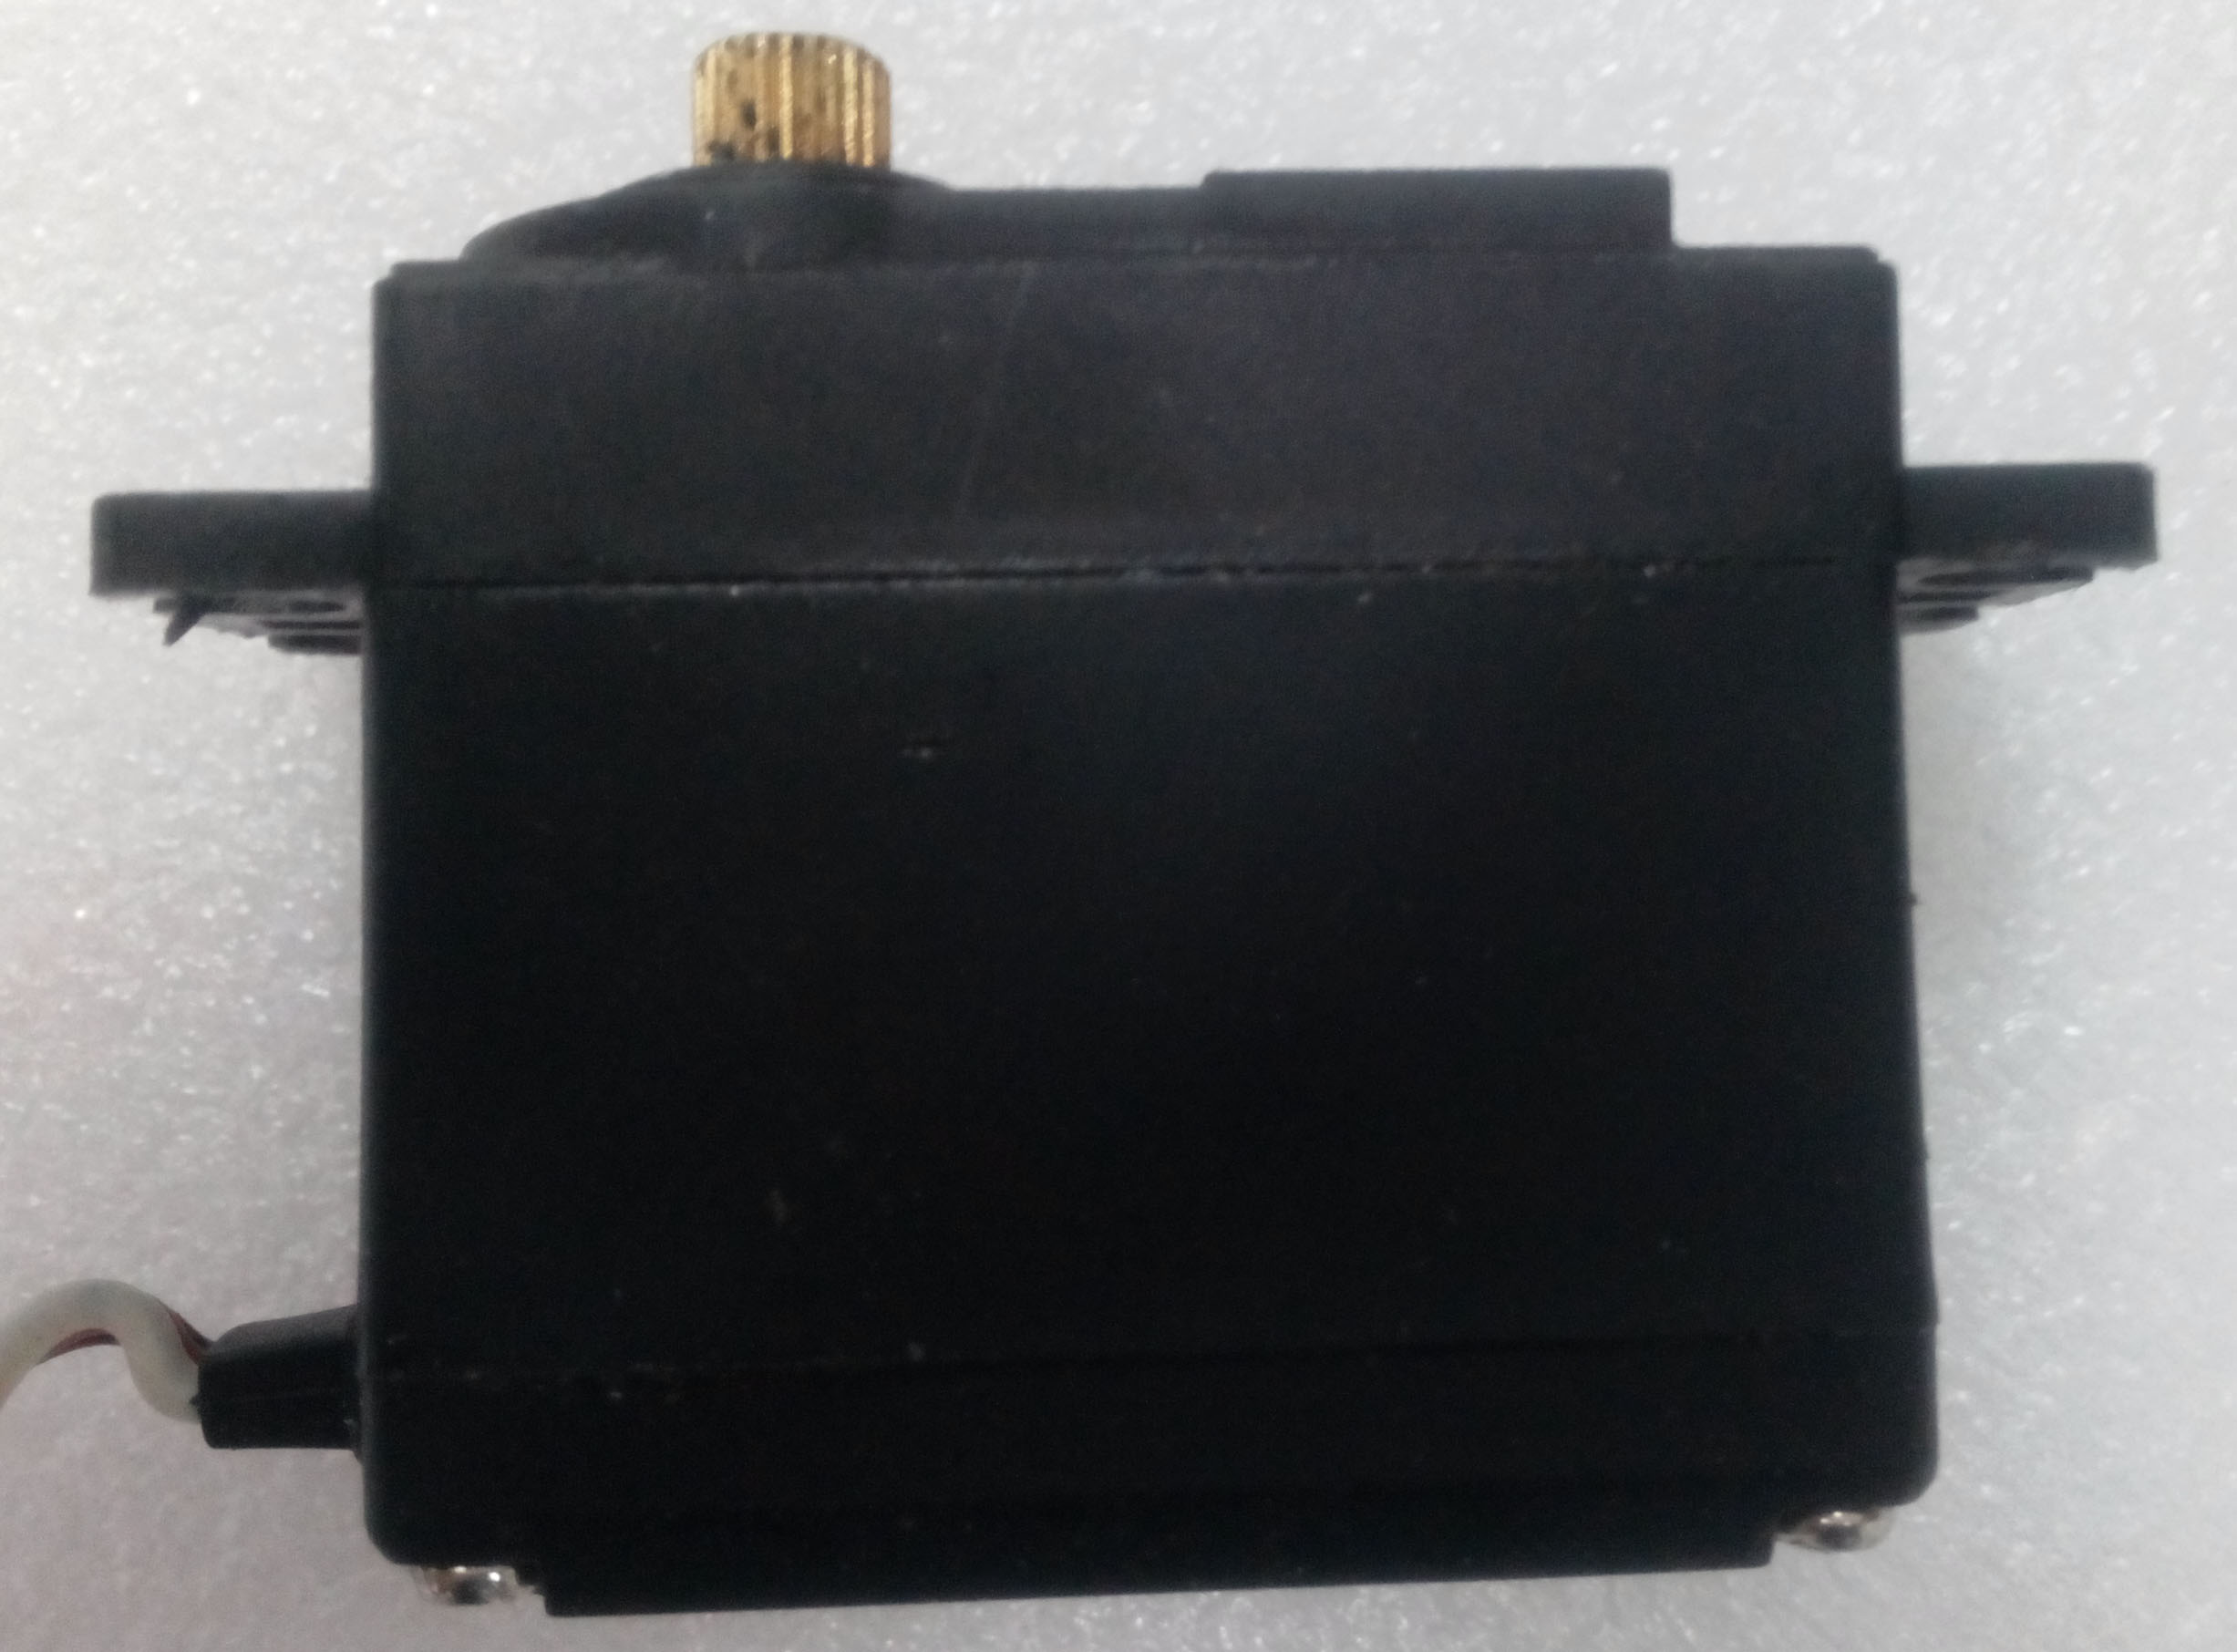
\includegraphics[width = 7cm,height= 6cm]{Servo.jpg}} 
	\hspace{2cm}
	\subfloat[Servo Bracket]{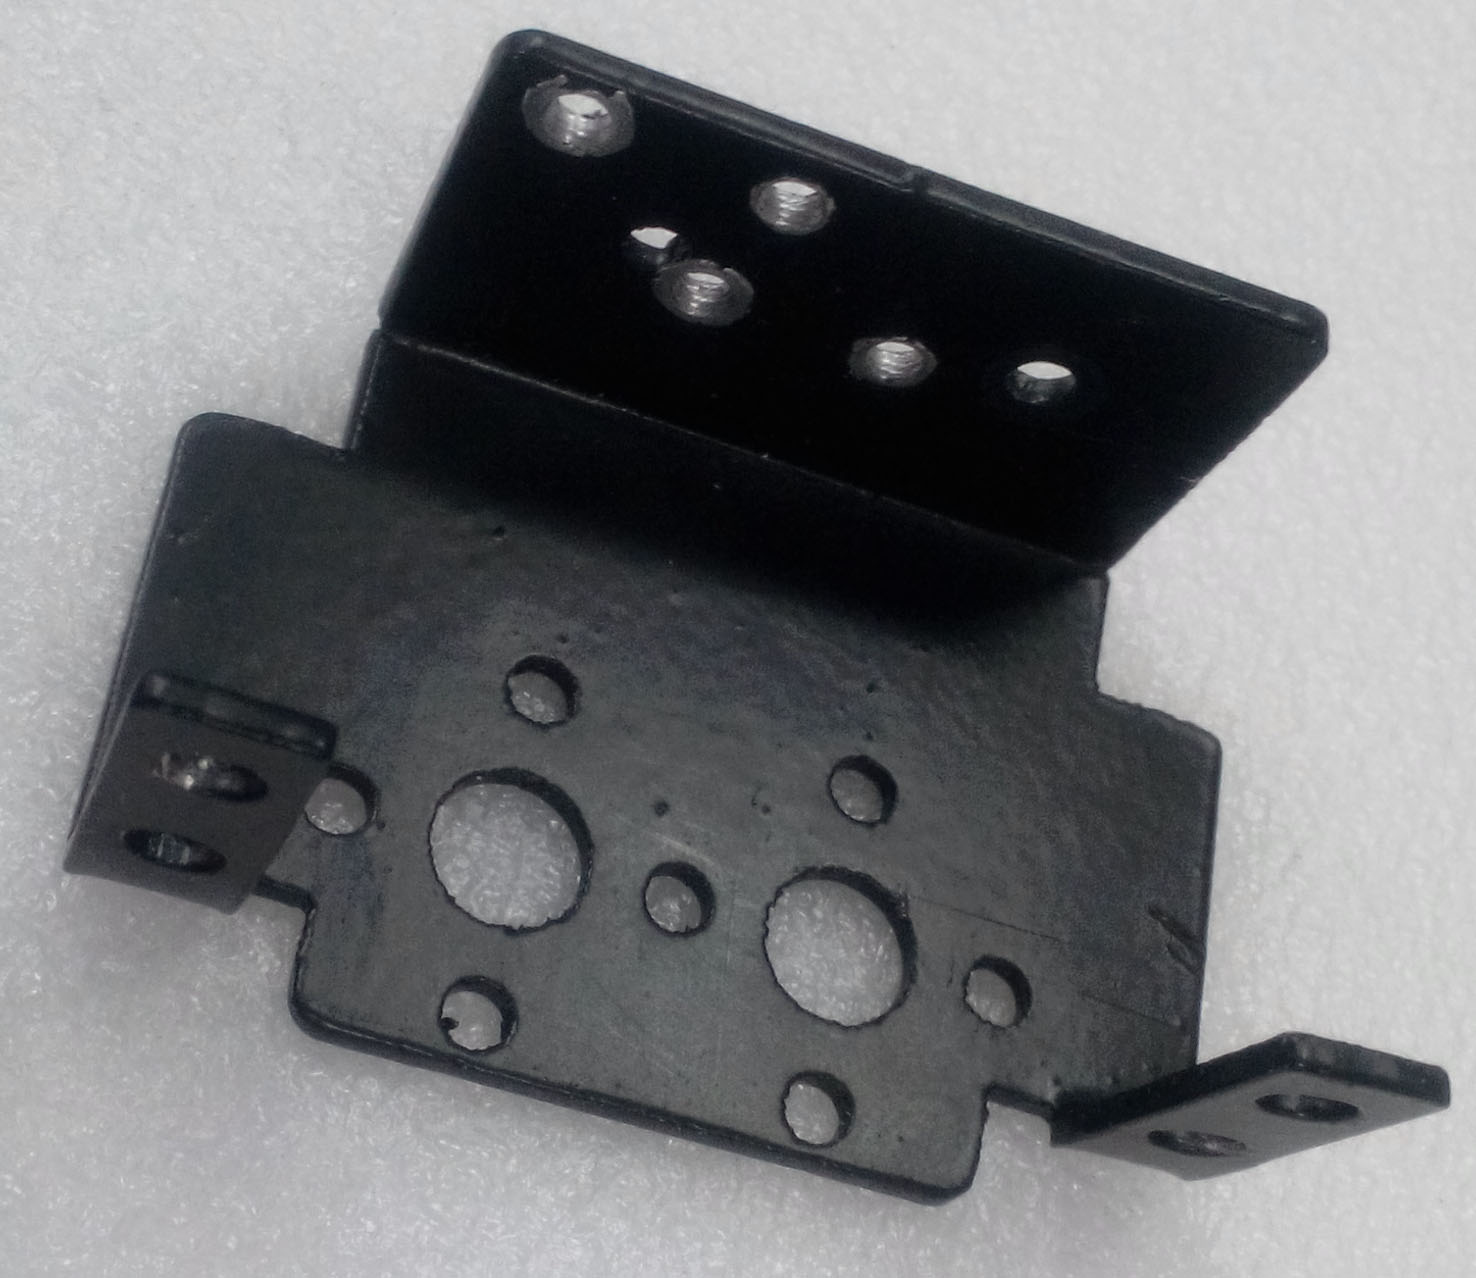
\includegraphics[width = 7cm,height= 6cm]{servo_bracket.jpg}}
	\newline
	\subfloat[C bracket Small]{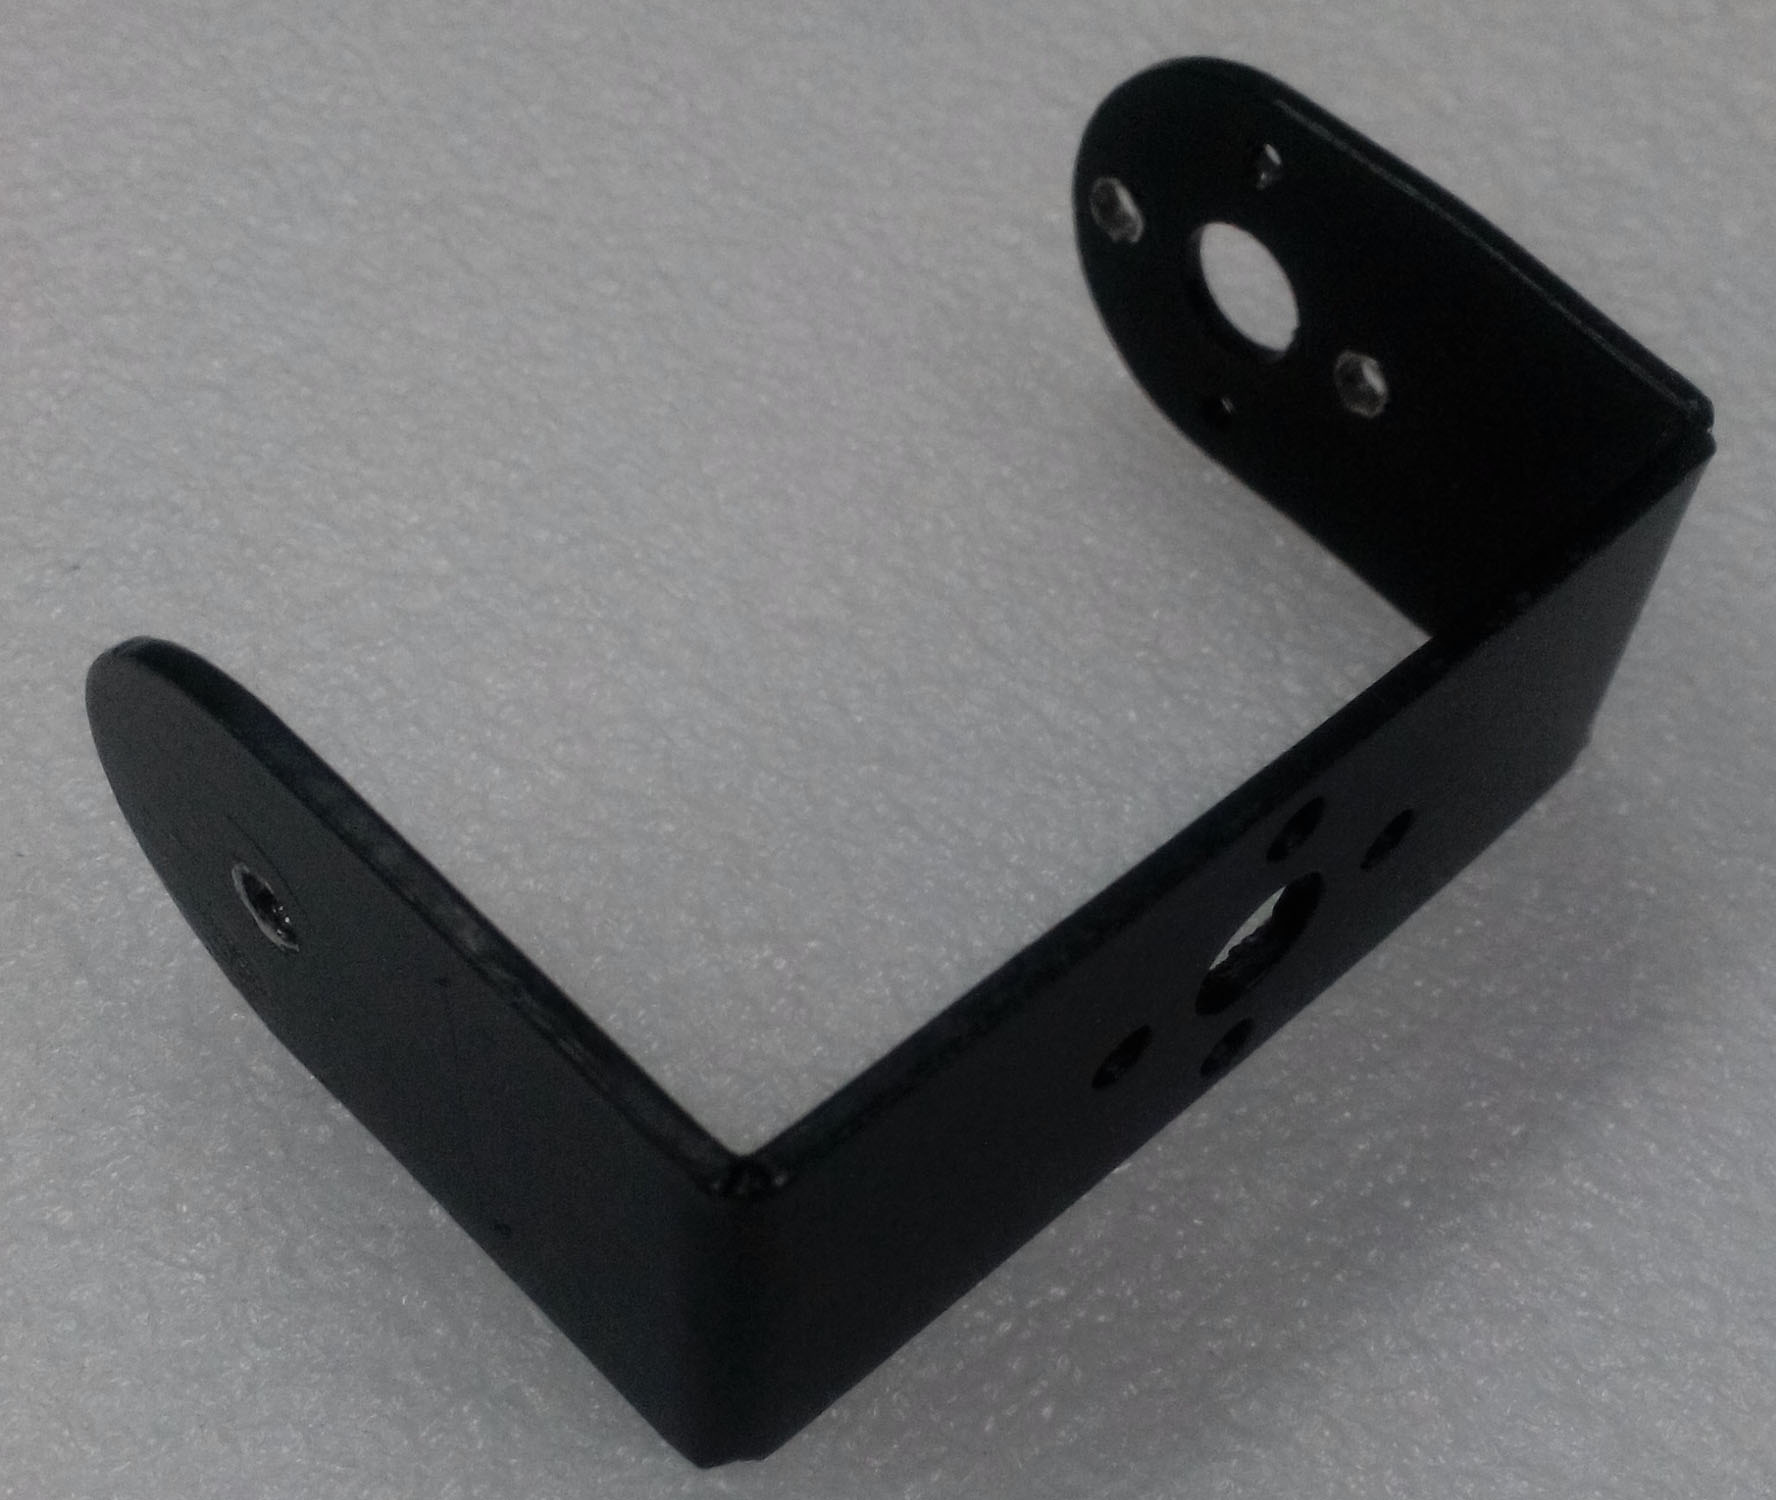
\includegraphics[width = 7cm,height= 6cm]{C_bracket_small.jpg}} 
	\hspace{2cm}
	\subfloat[C bracket Long]{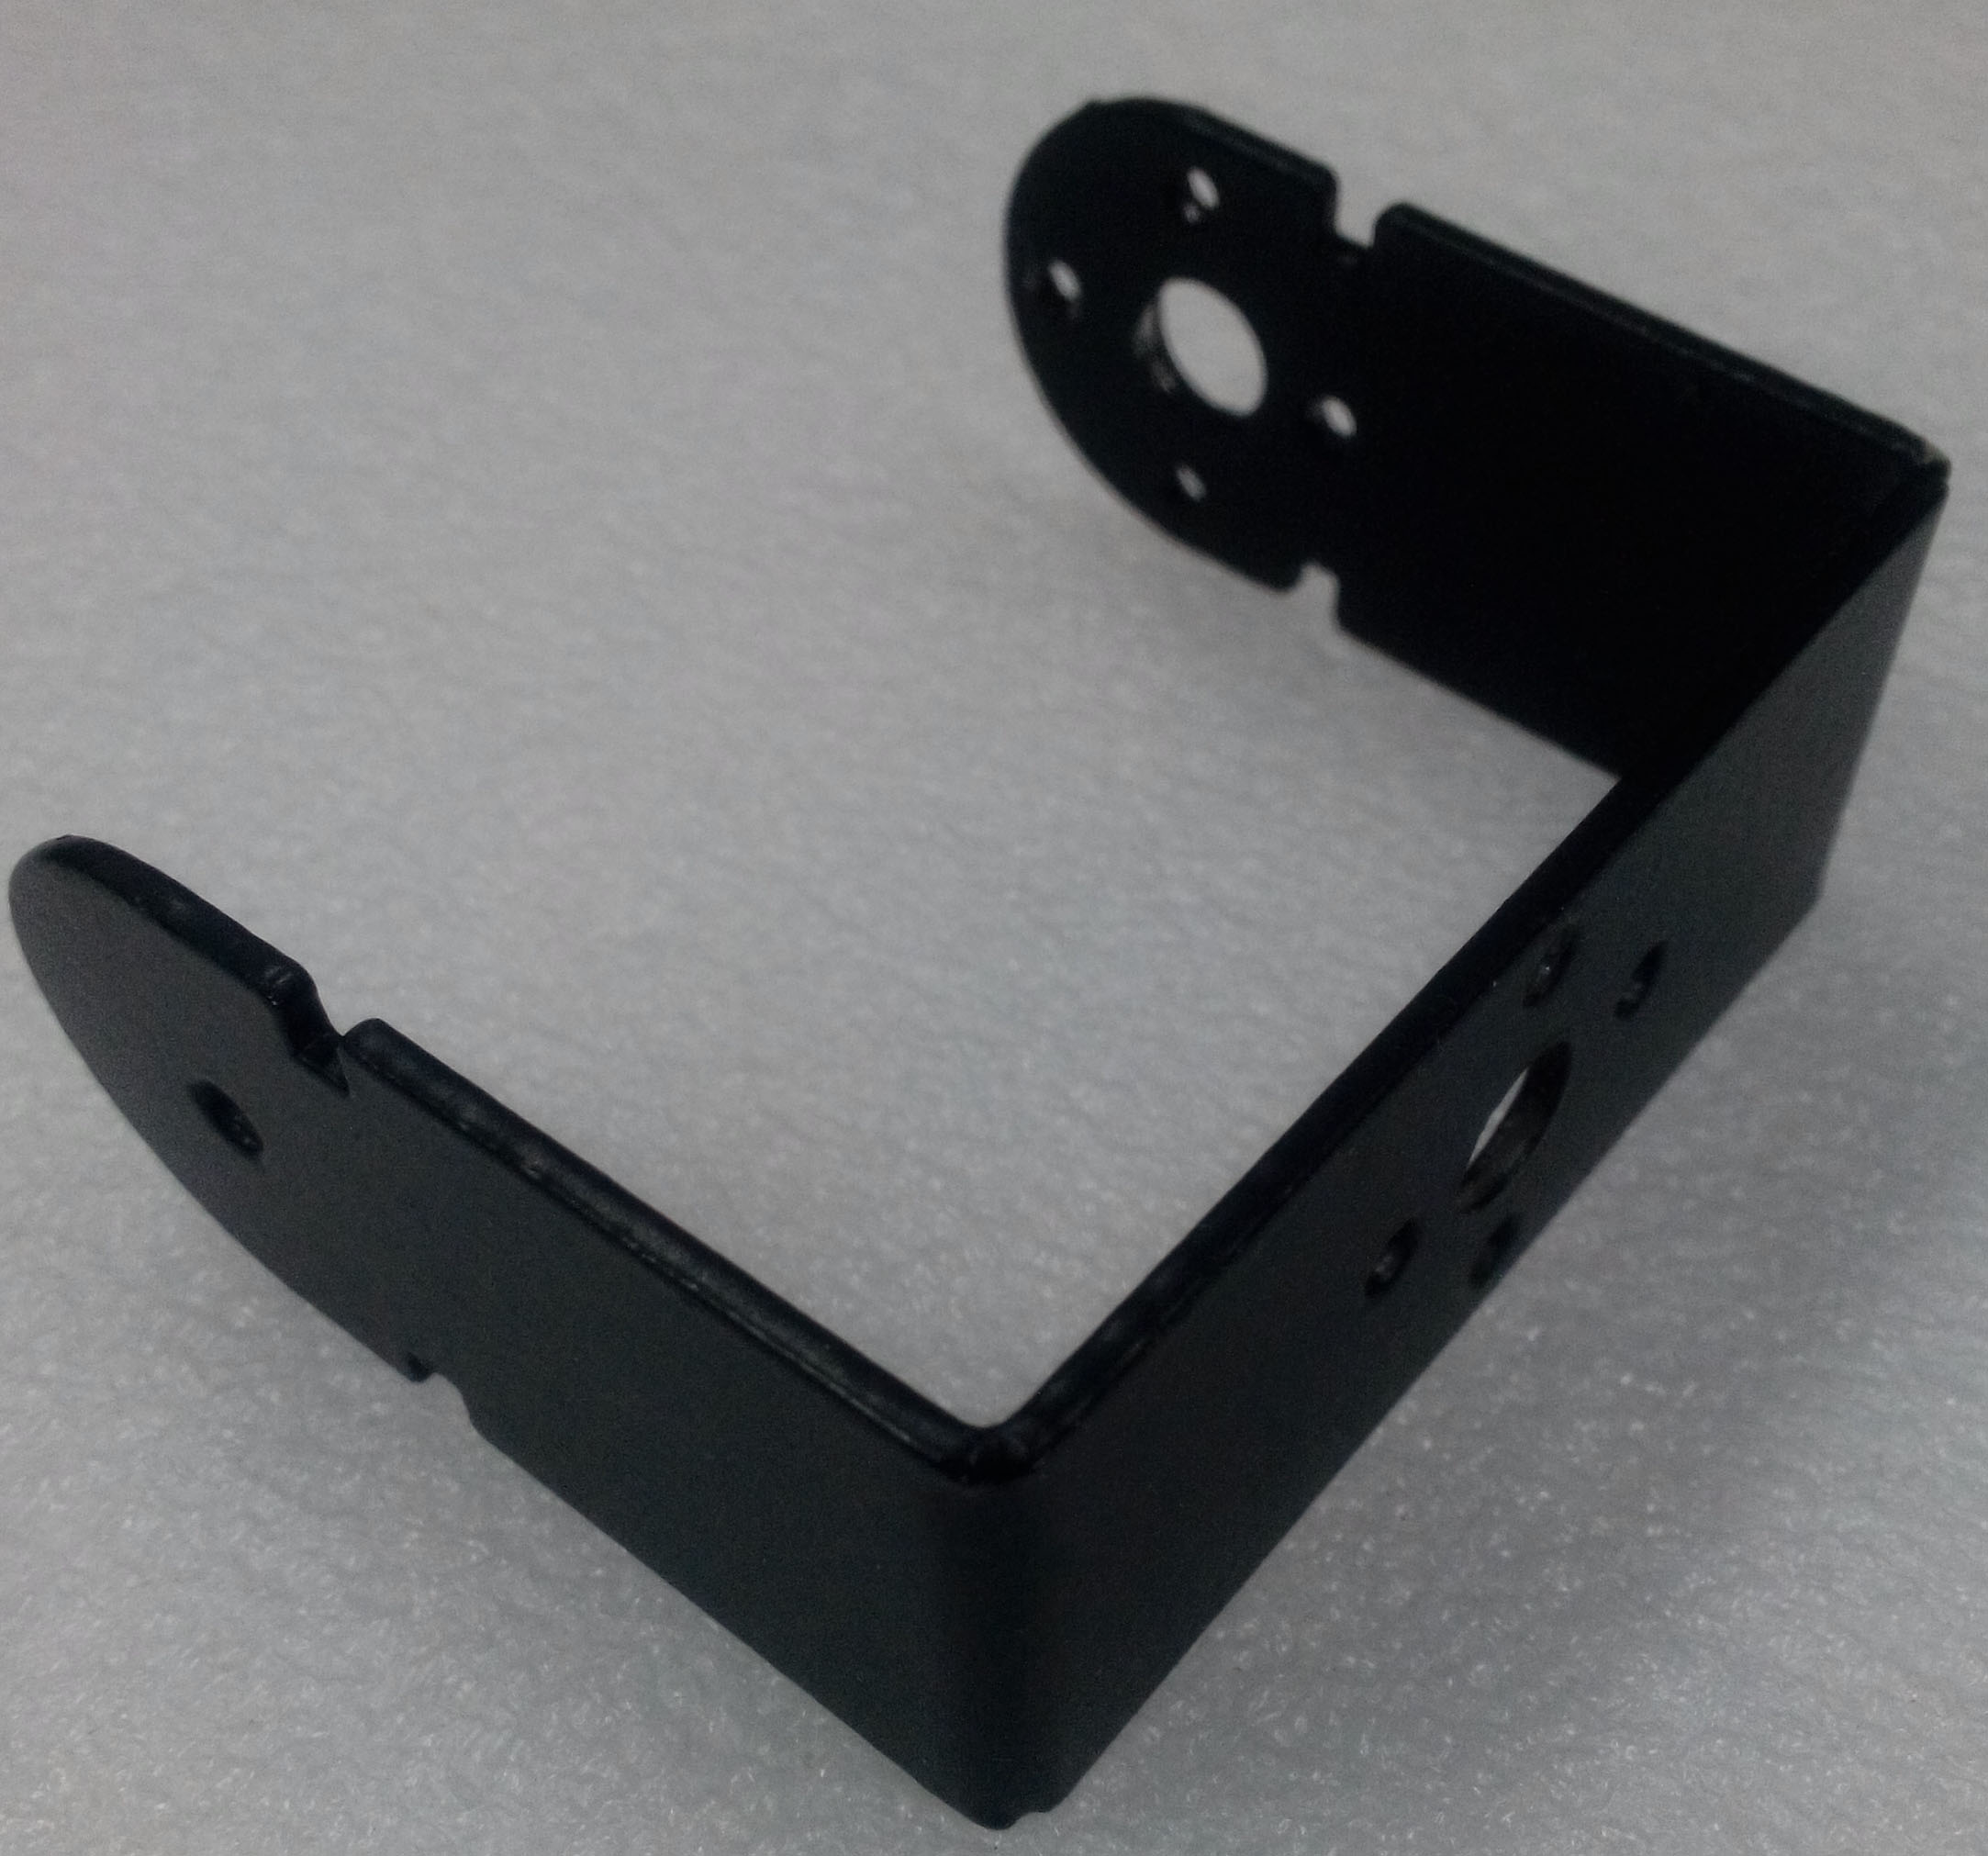
\includegraphics[width = 7cm,height= 6cm]{C_bracket_long.jpg}}
	\caption{List of components}
\end{figure}
\newpage
\begin{figure}[h!]
	\ContinuedFloat
	\centering
	\subfloat[C bracket Hand]{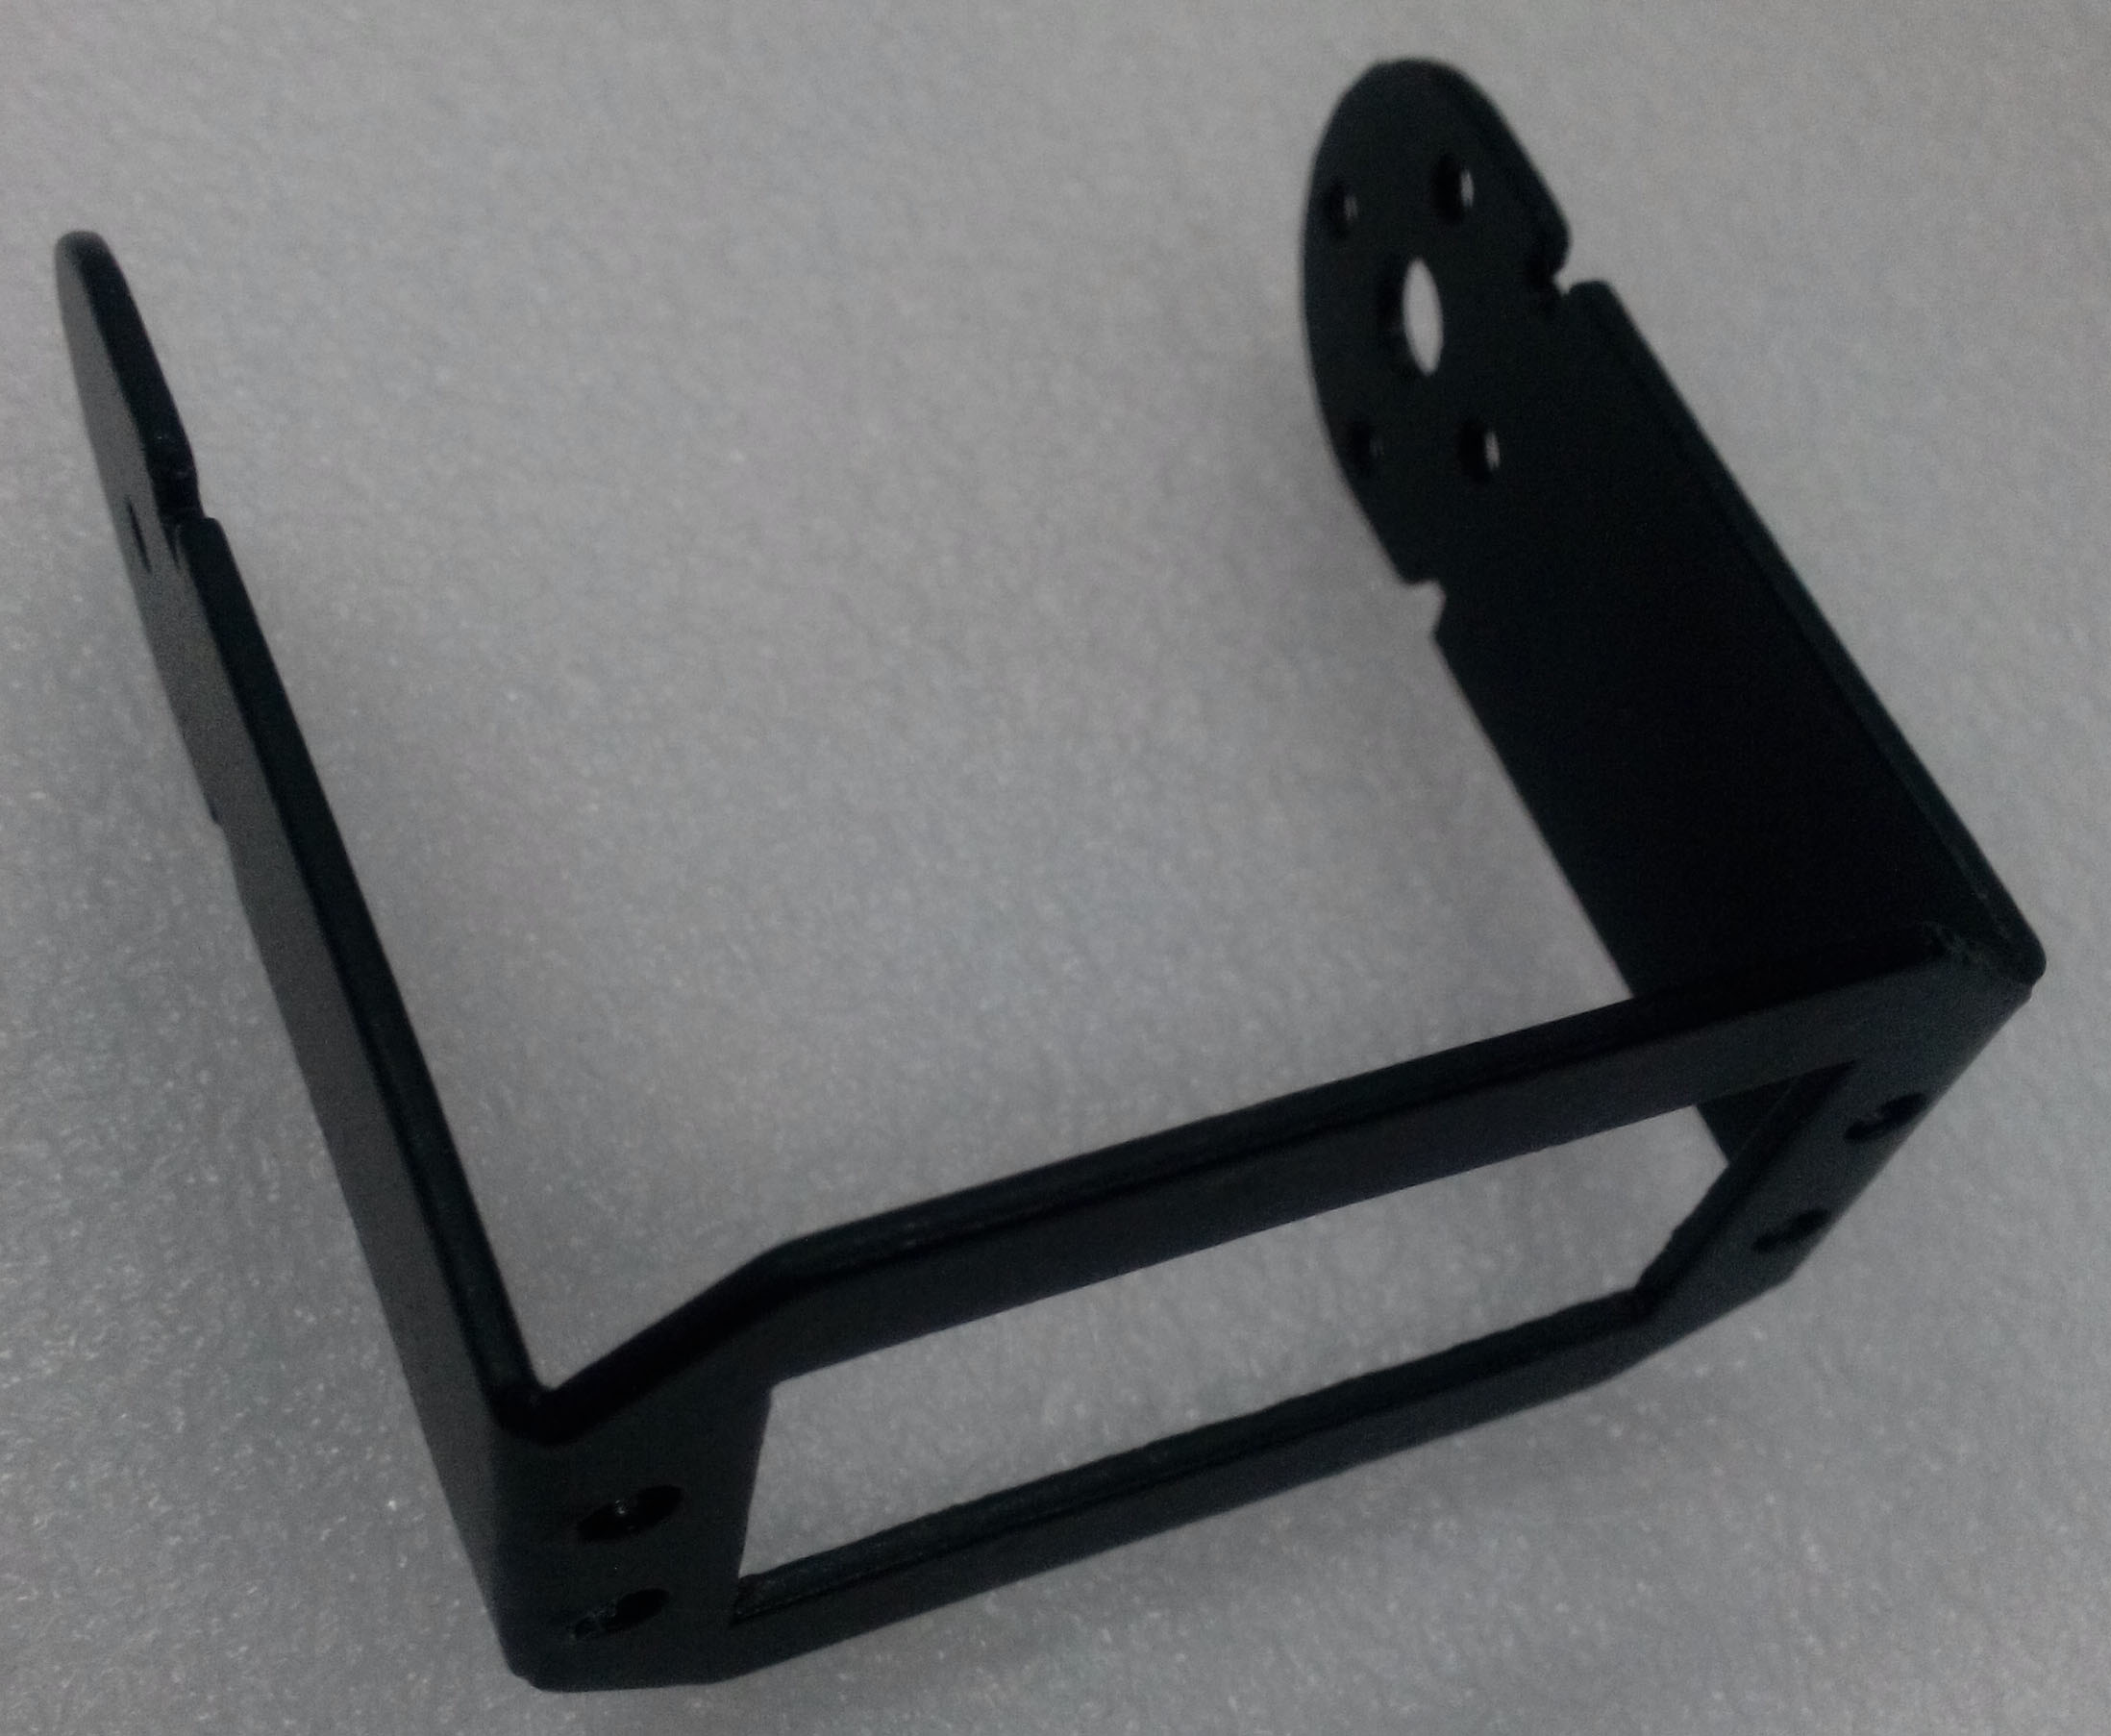
\includegraphics[width = 7cm,height= 6cm]{handCbraket.jpg}} 
	\hspace{2cm}
	\subfloat[L bracket]{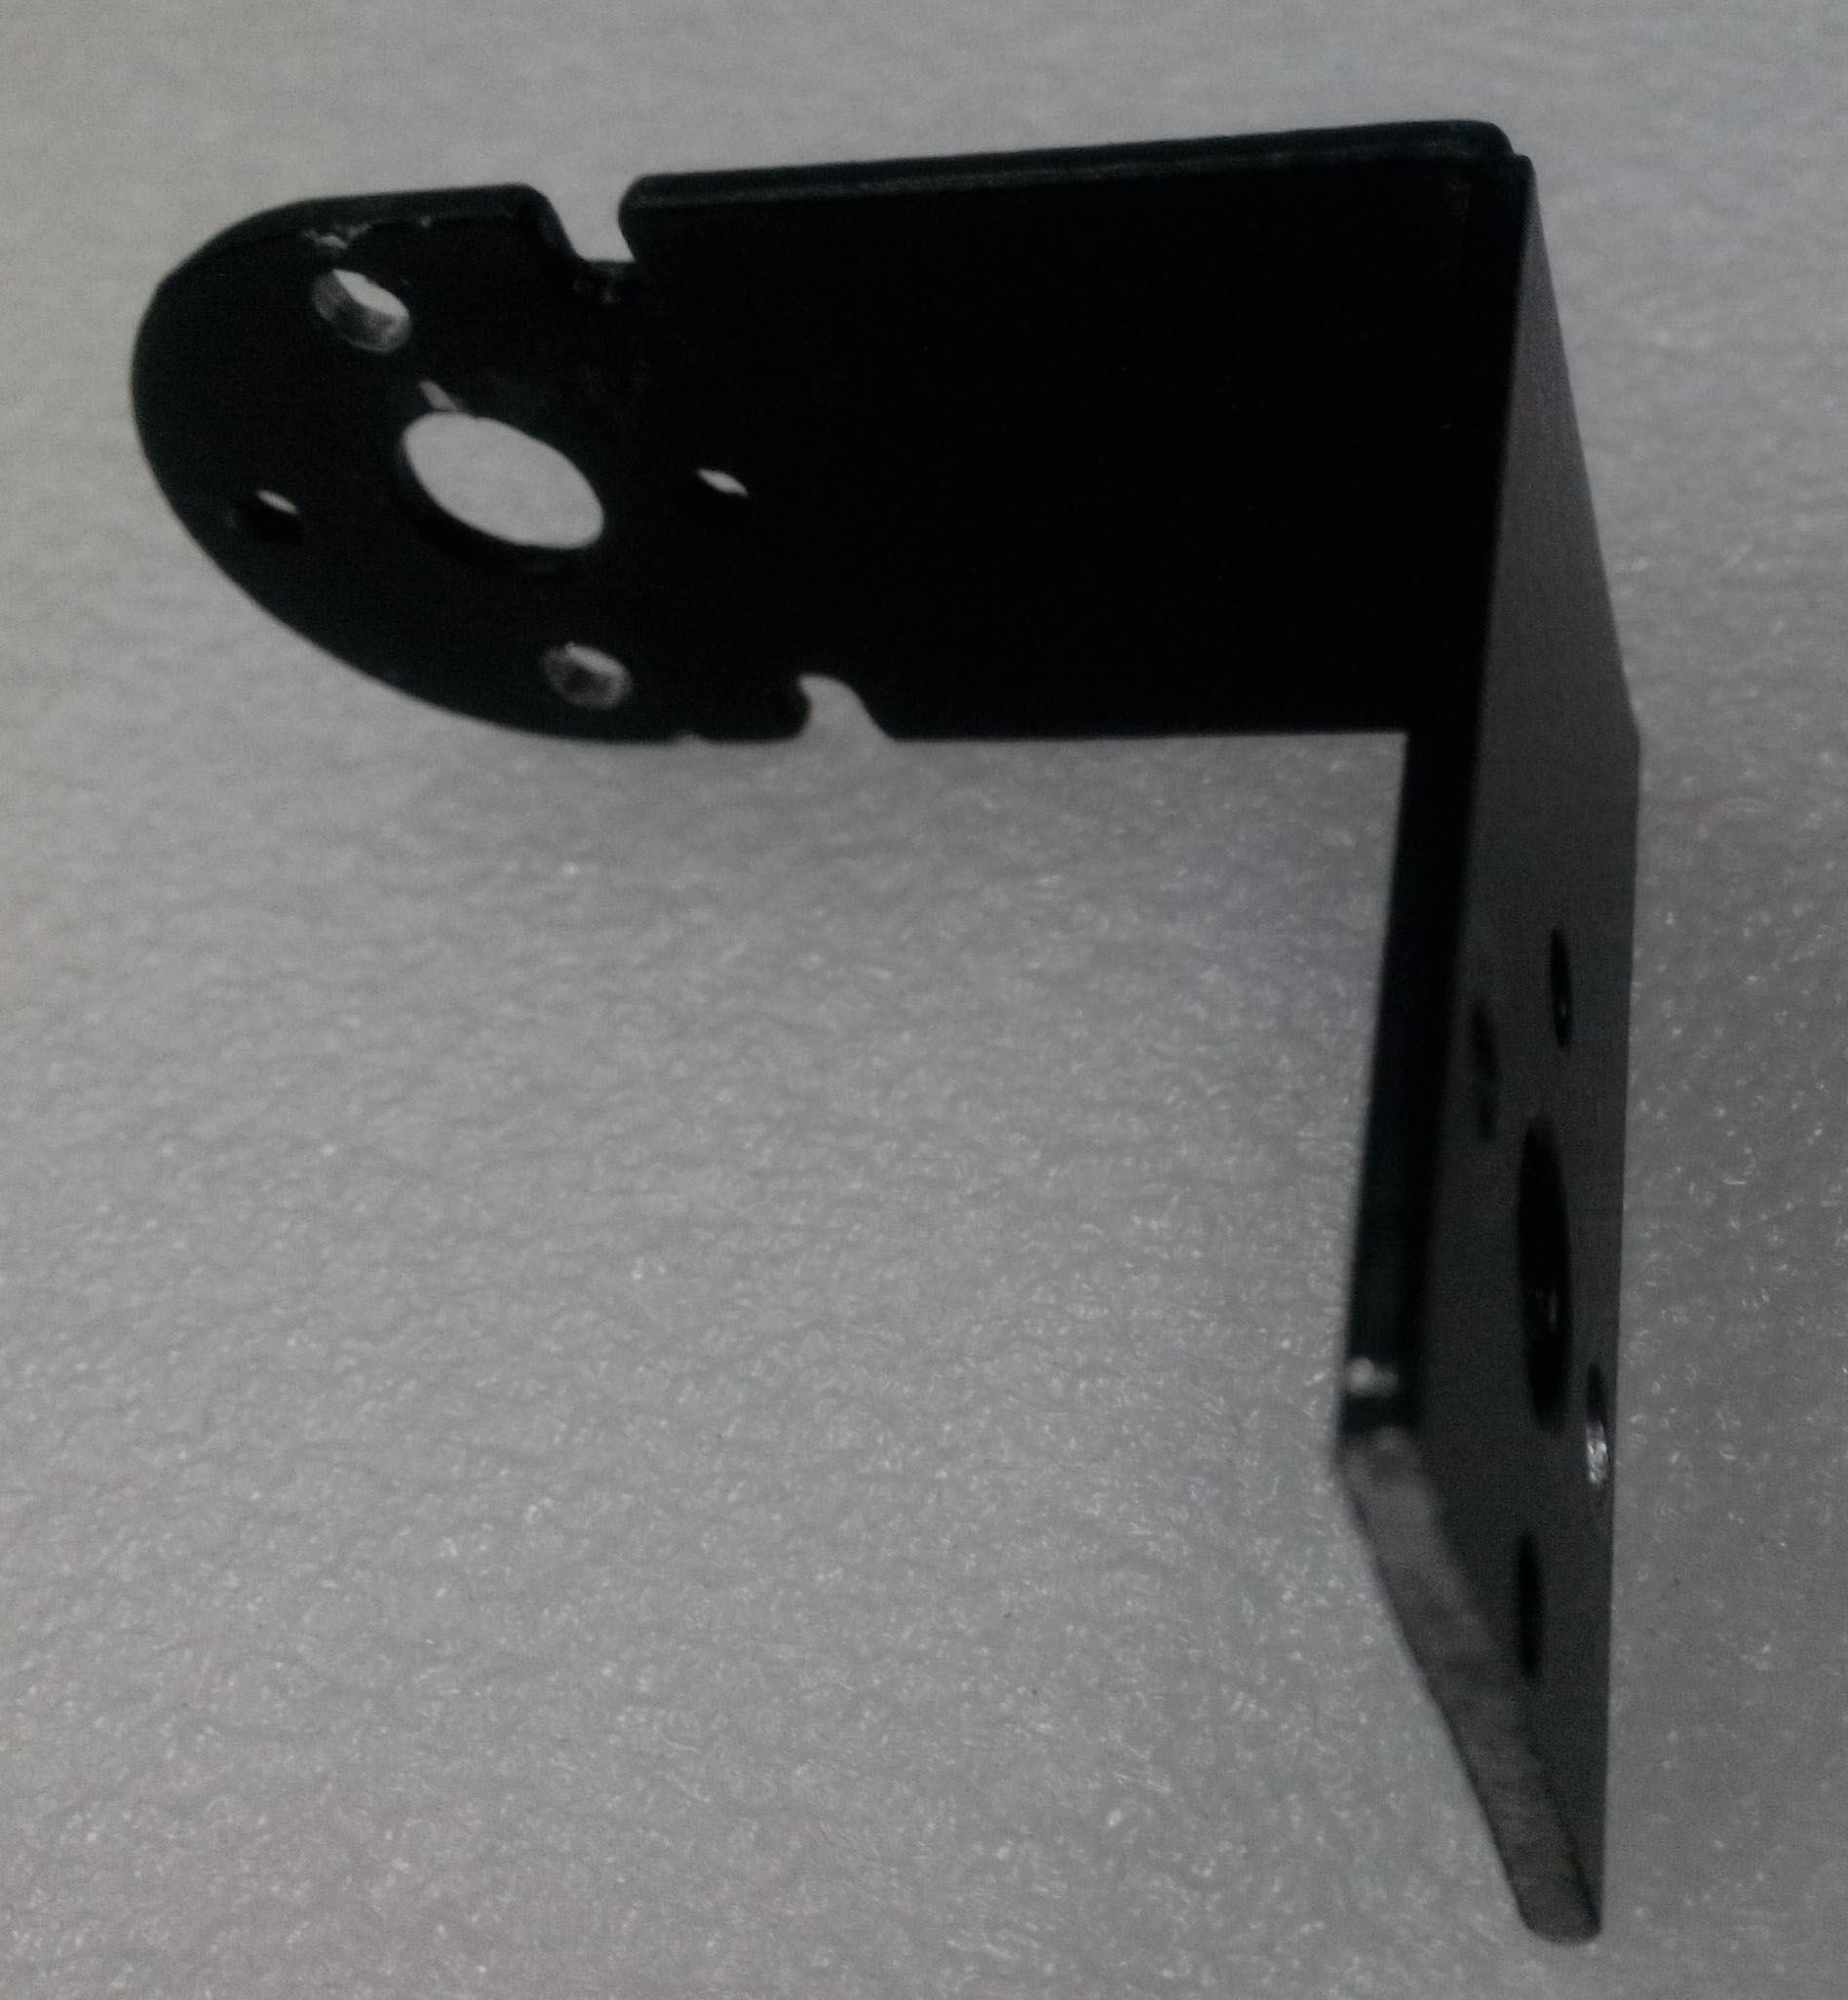
\includegraphics[width = 7cm,height= 6cm]{L_bracket.jpg}}
	\newline
	\subfloat[Servo Flap]{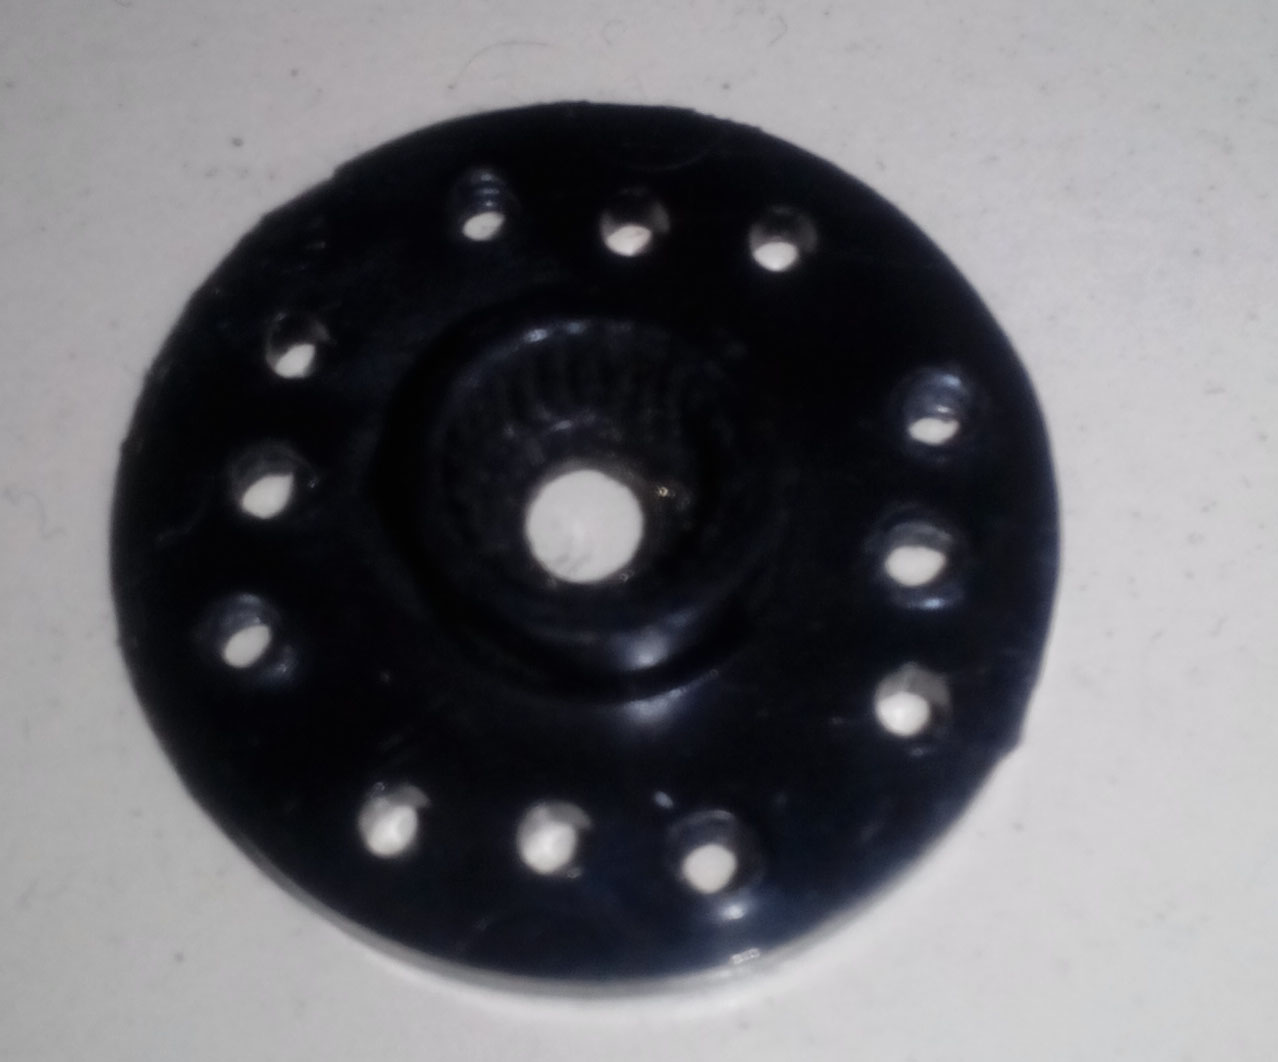
\includegraphics[width = 7cm,height= 6cm]{flap.jpg}} 
	\hspace{2cm}
	\subfloat[Screws]{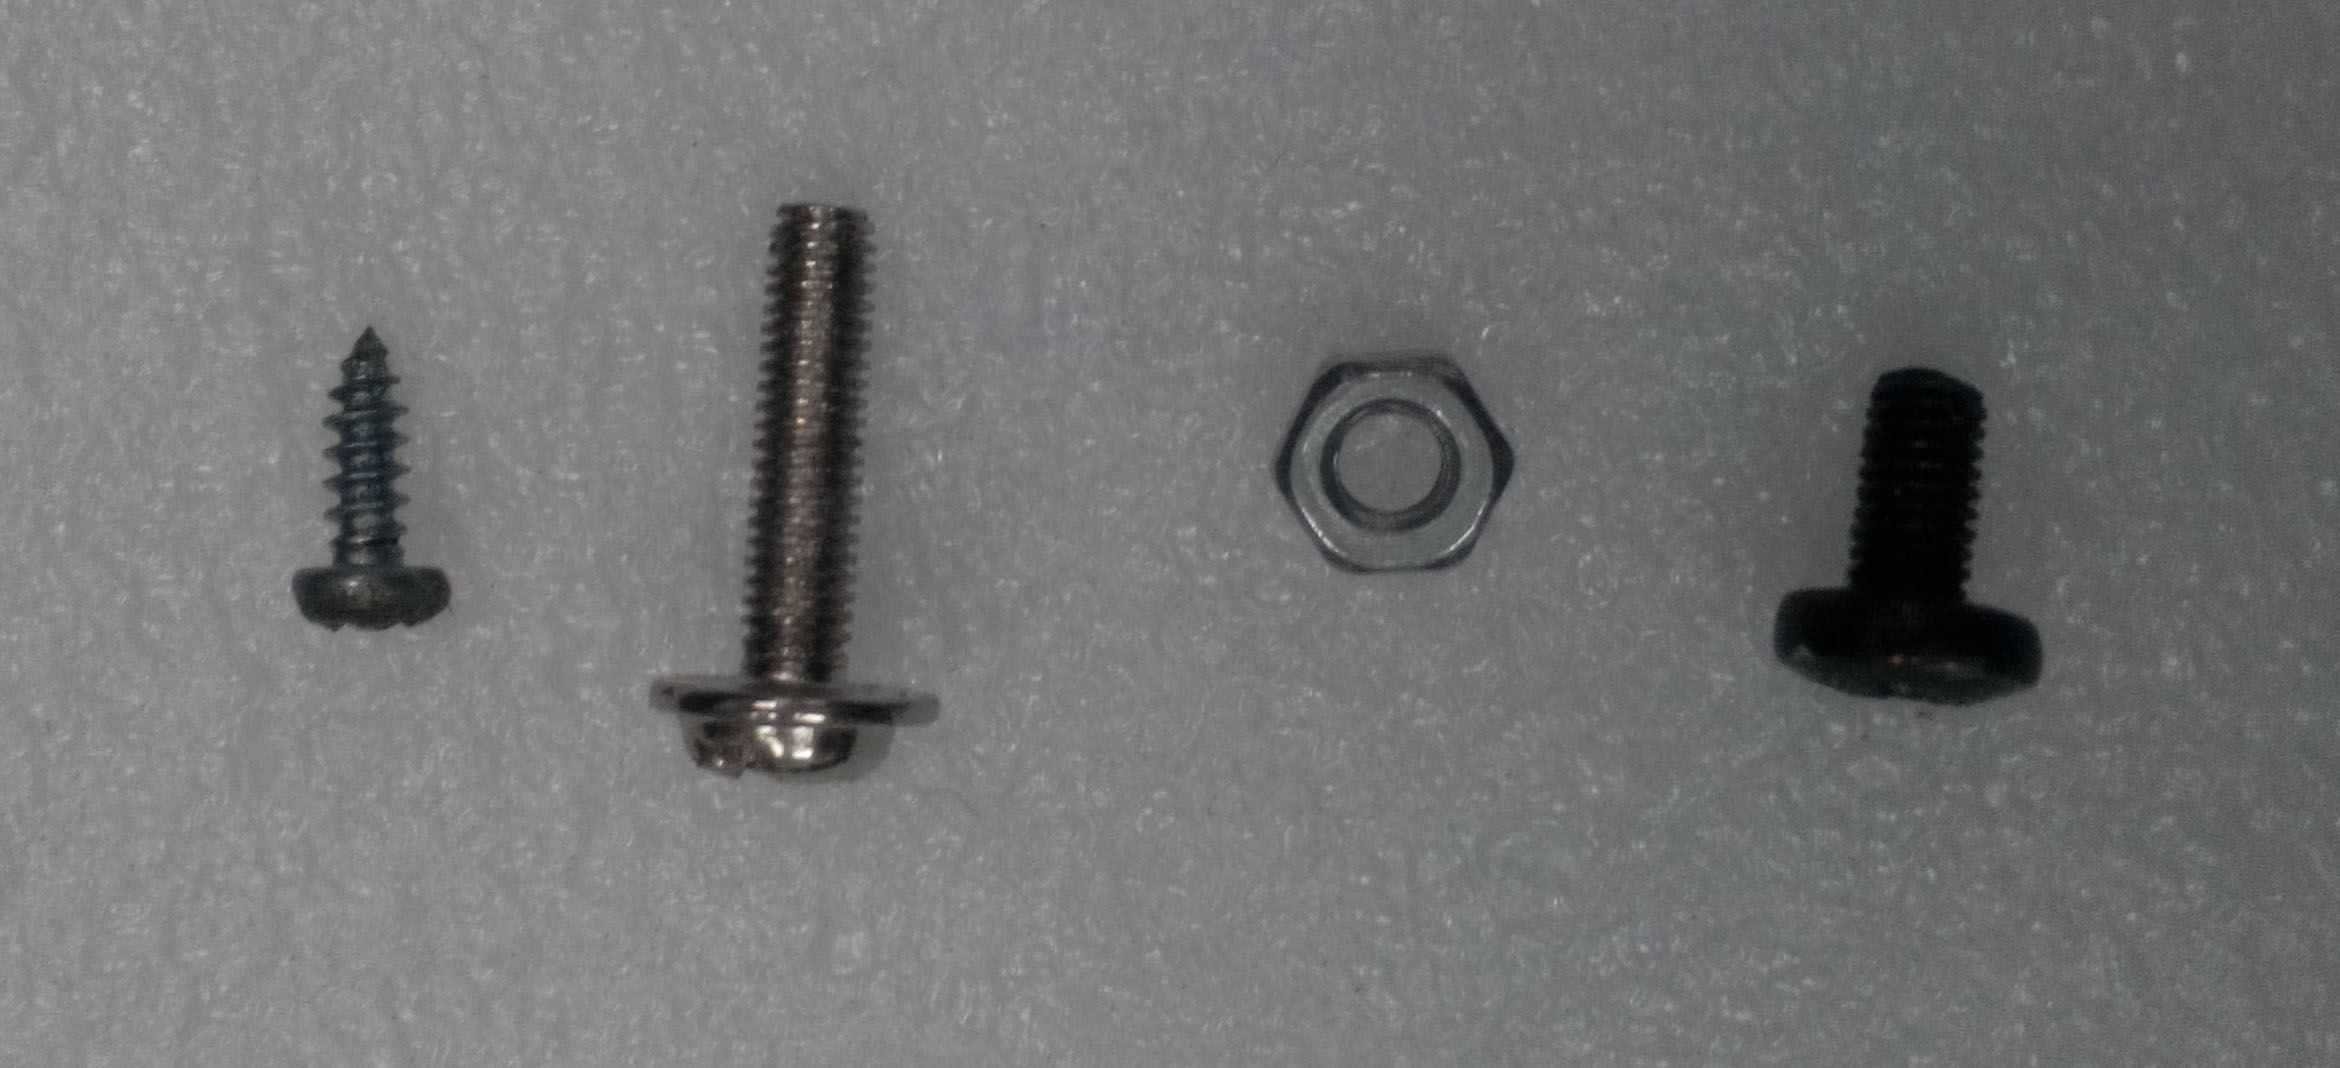
\includegraphics[width = 7cm,height= 6cm]{screws.jpg}}
	\hspace{2cm}
	\subfloat[Hard Polymer]{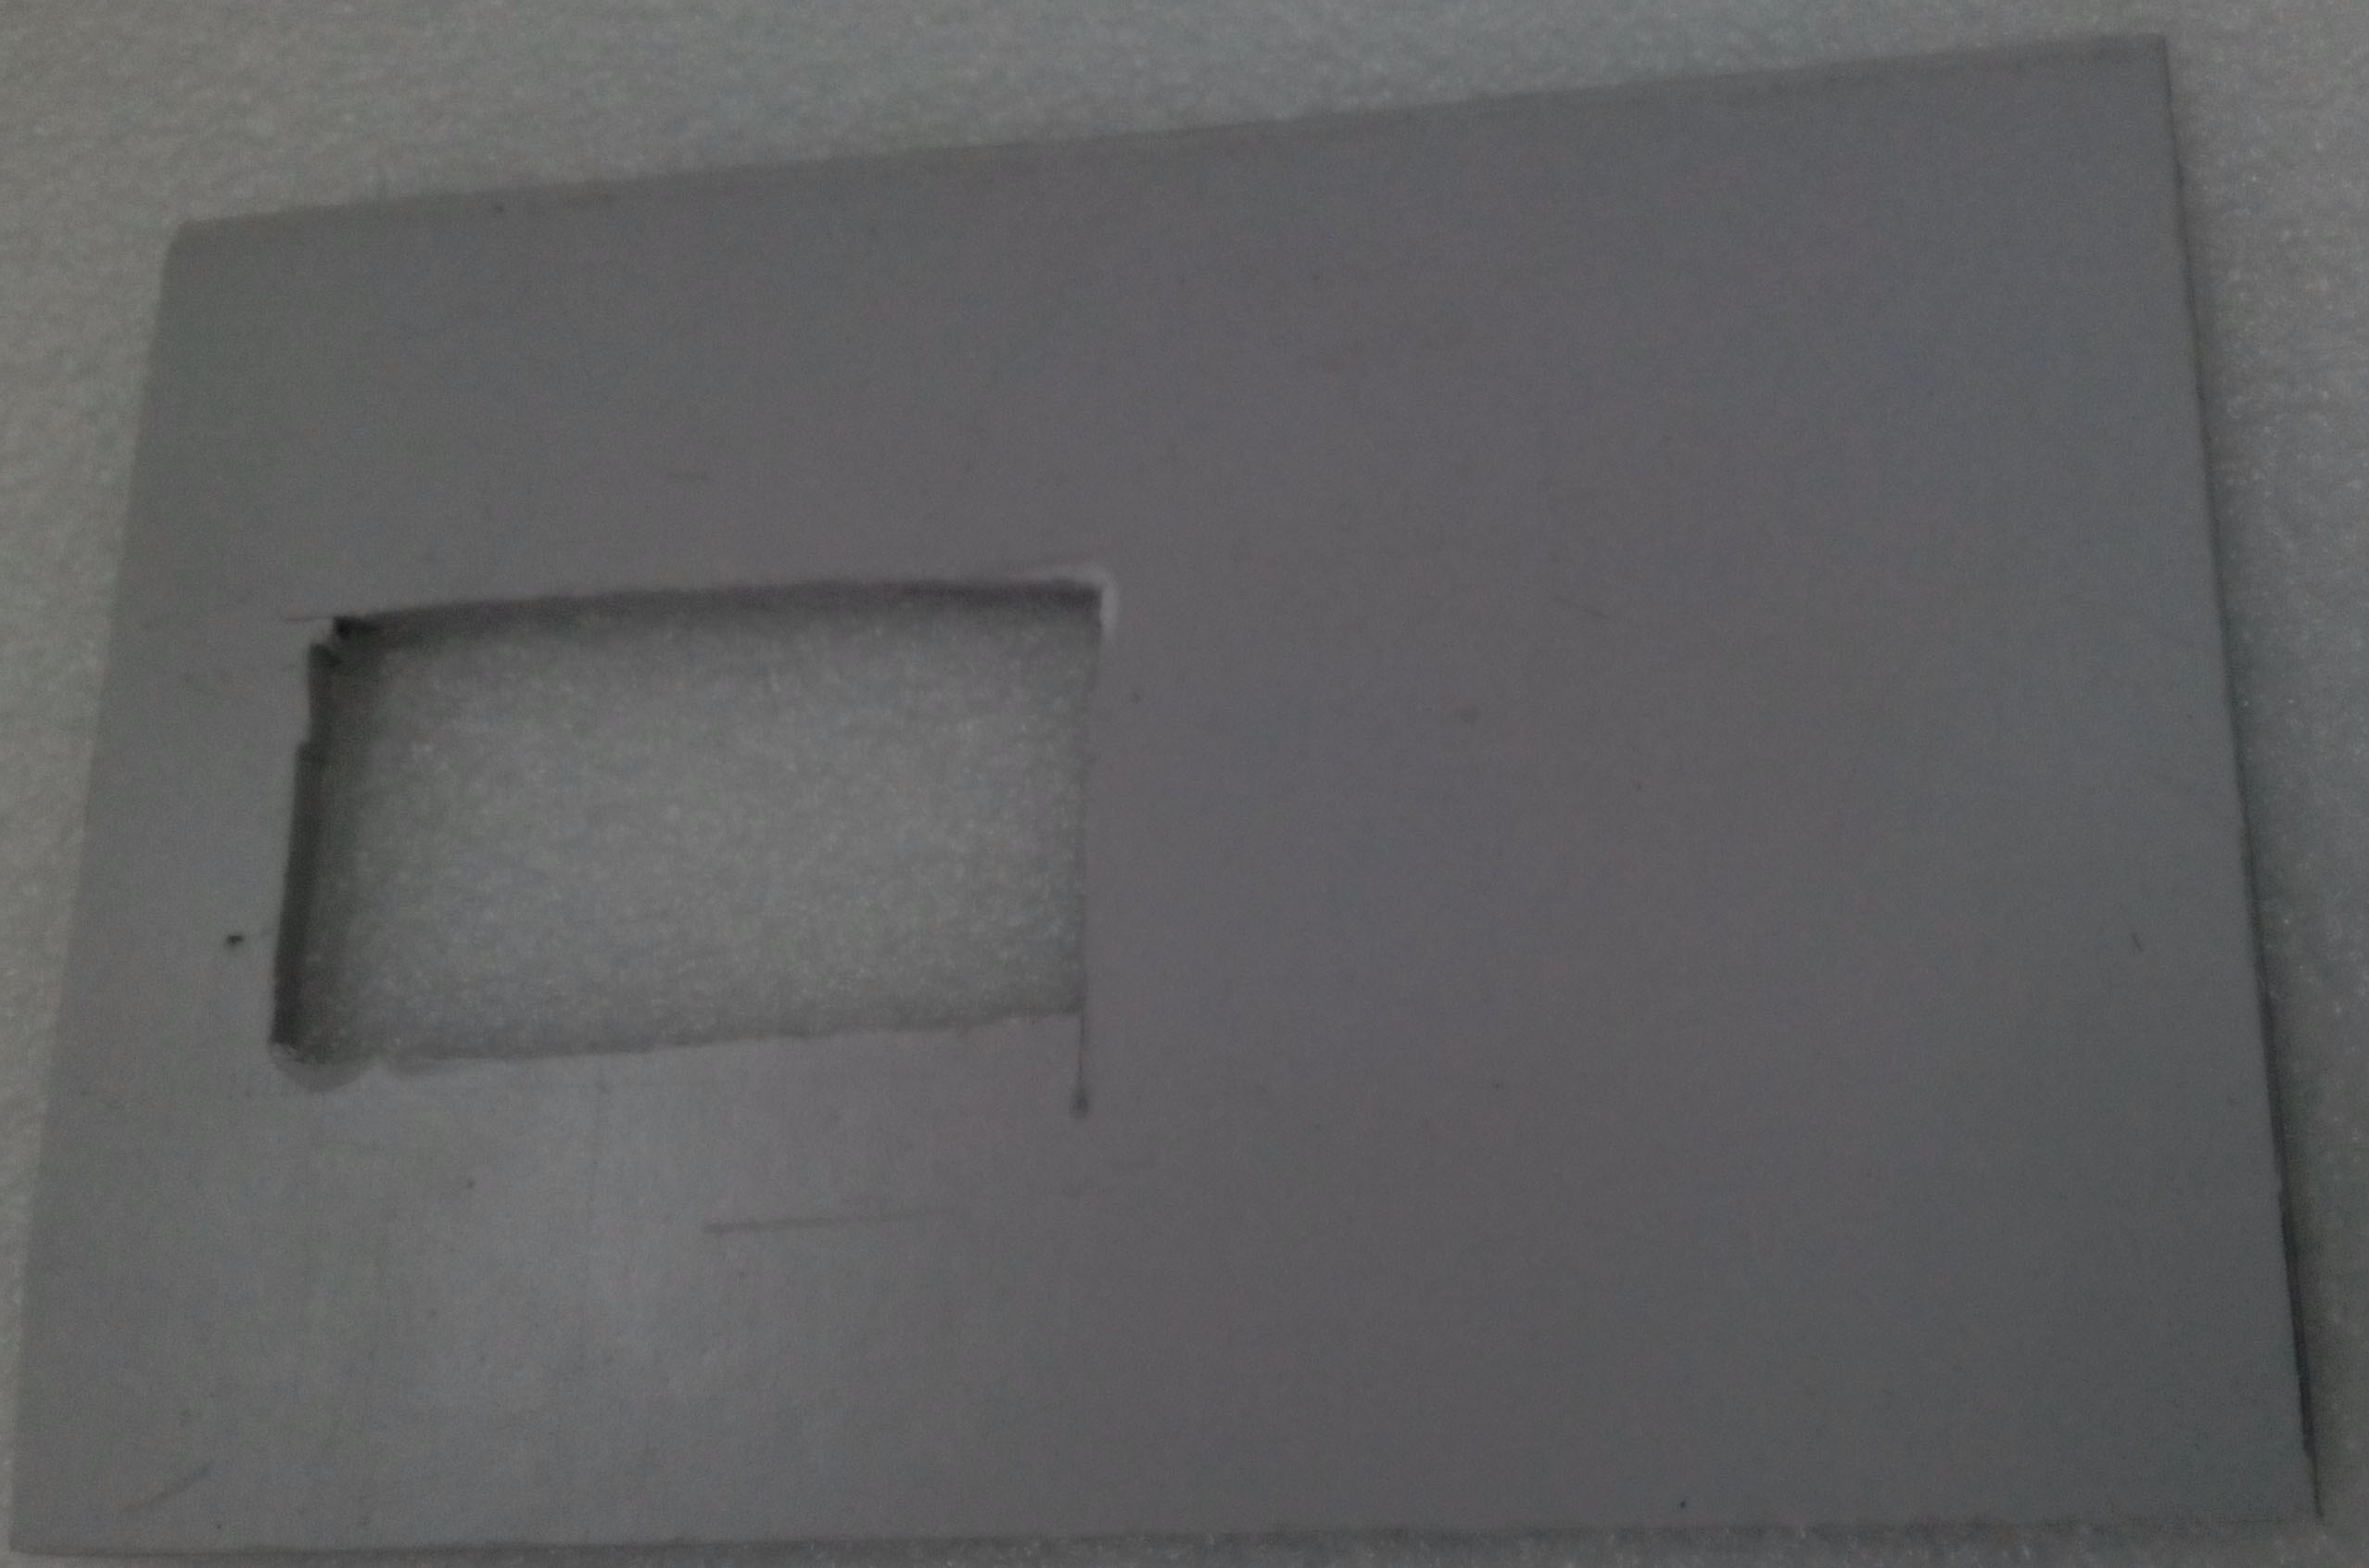
\includegraphics[width = 7cm,height= 6cm]{polystyrine.jpg}}
	\caption{List of components}
\end{figure}
\newpage
\subsubsection{Problem faced in finding appropriate component}
The component [c] which is the C bracket Small was either out of stock or not available in
the market. So we had to 3D print the bracket. We have used Autodesk 123Design which
is open source software specially meant for 3D design printing, to model the bracket
design. To print the design Makers BOT 3D printer was used available at ERTS lab IIT
Bombay.
\begin{figure}[h!]
	\centering
	\subfloat[Snapshot of the Design]{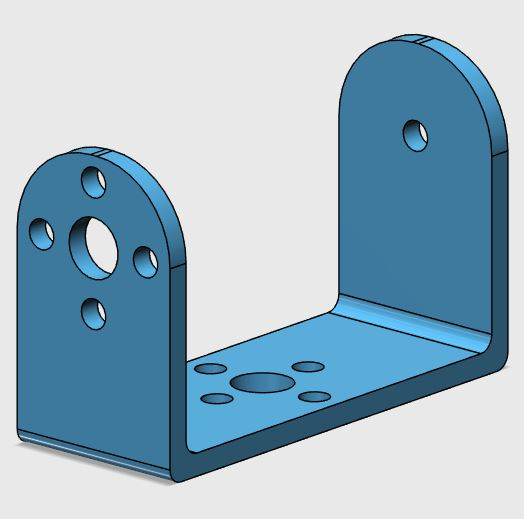
\includegraphics[width = 7cm,height= 6cm]{bracket.jpg}} 
	\hspace{2cm}
	\subfloat[3D Printed bracket]{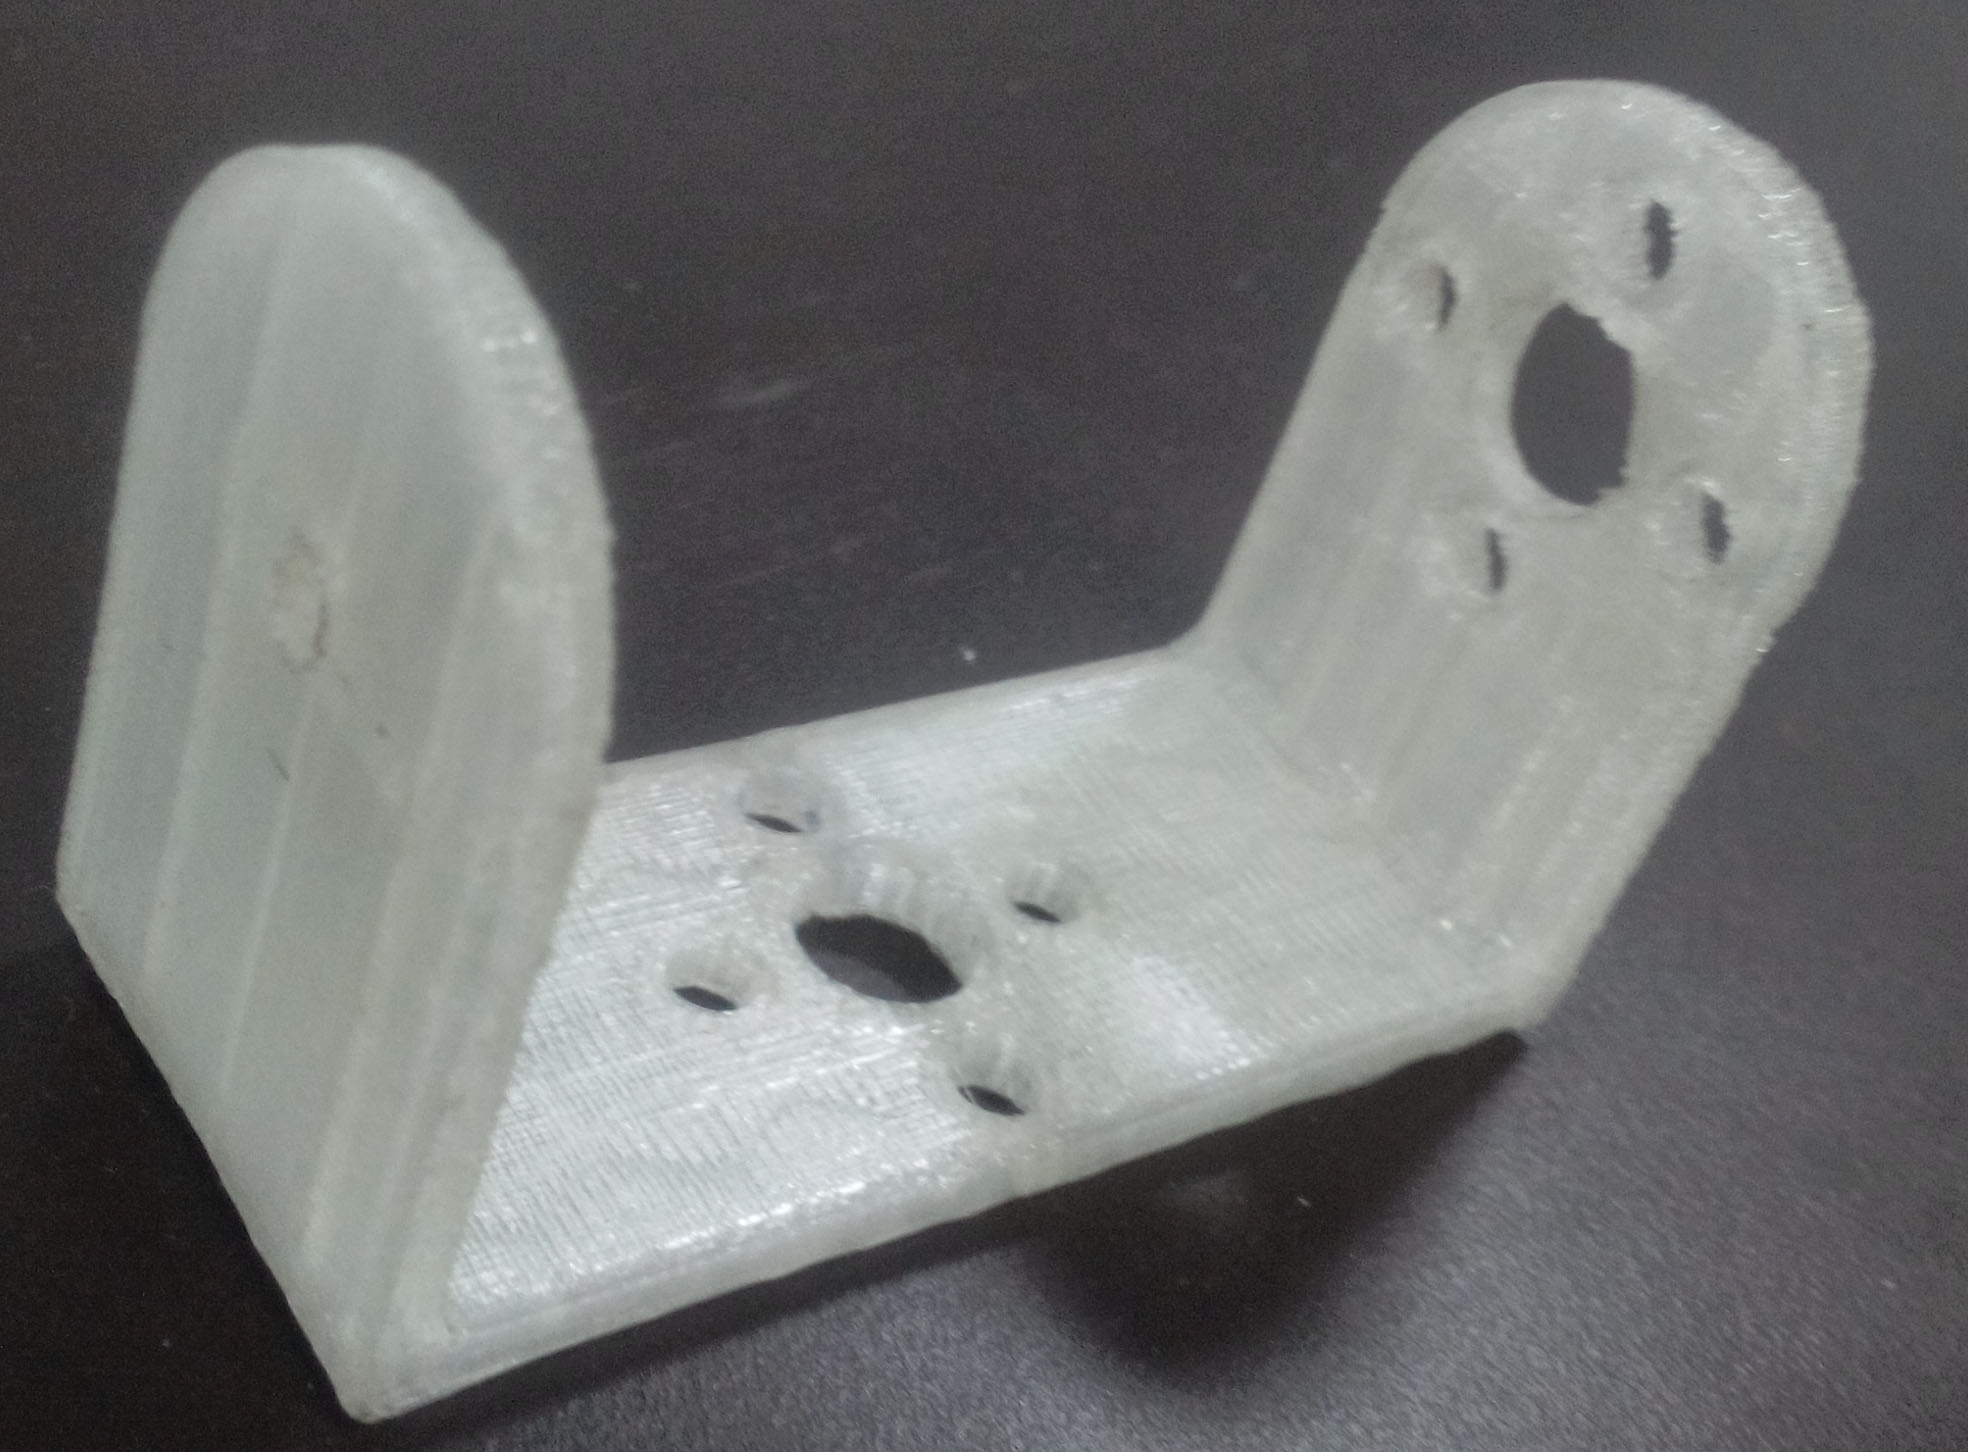
\includegraphics[width = 7cm,height= 6cm]{C_bracket_small_3D_printed.jpg}}
	\newline
	
	\caption{3D printed component}
\end{figure}

\subsubsection{Assembly}
Now, coming to the construction and the assembly part first the basic links are prepared
using the various brackets listed above.\\
Some basic links with Images are listed below:\\
\begin{figure}[h!]
	\centering
	\subfloat[Servo mounted on bracket]{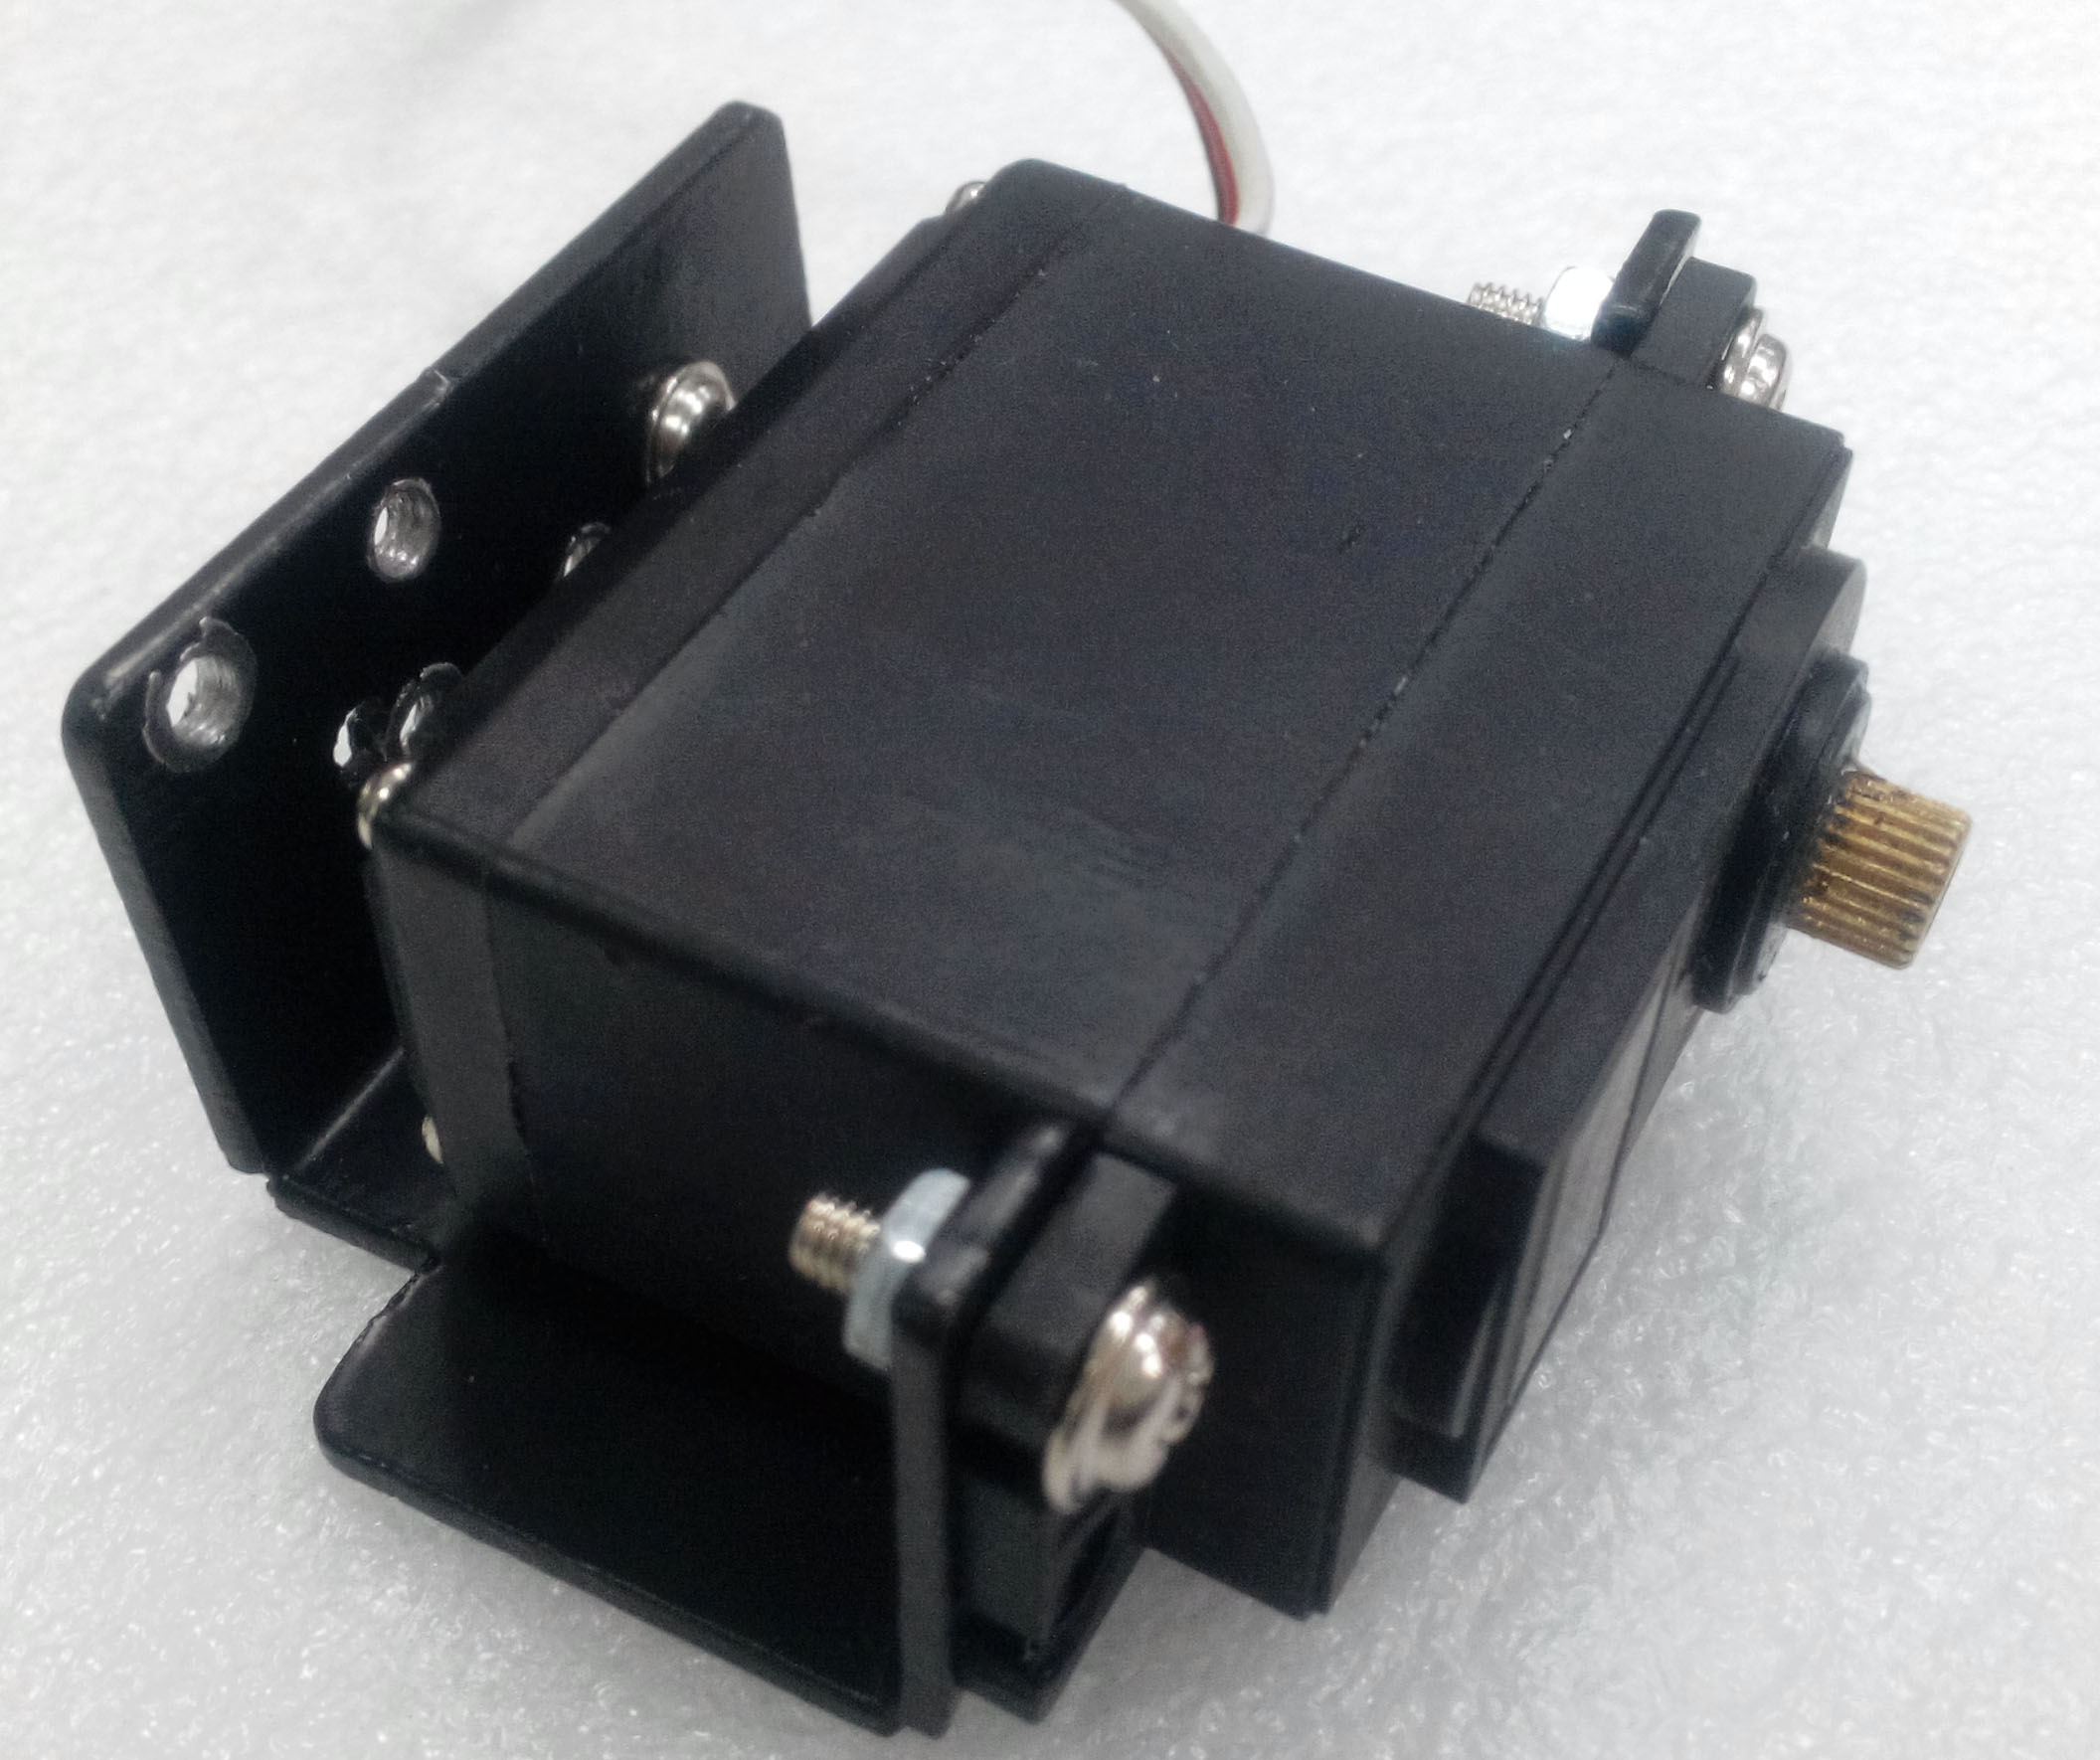
\includegraphics[width = 7cm,height= 6cm]{mountedservo.jpg}} 
	\hspace{2cm}
	\subfloat[C bracket with Flap attached]{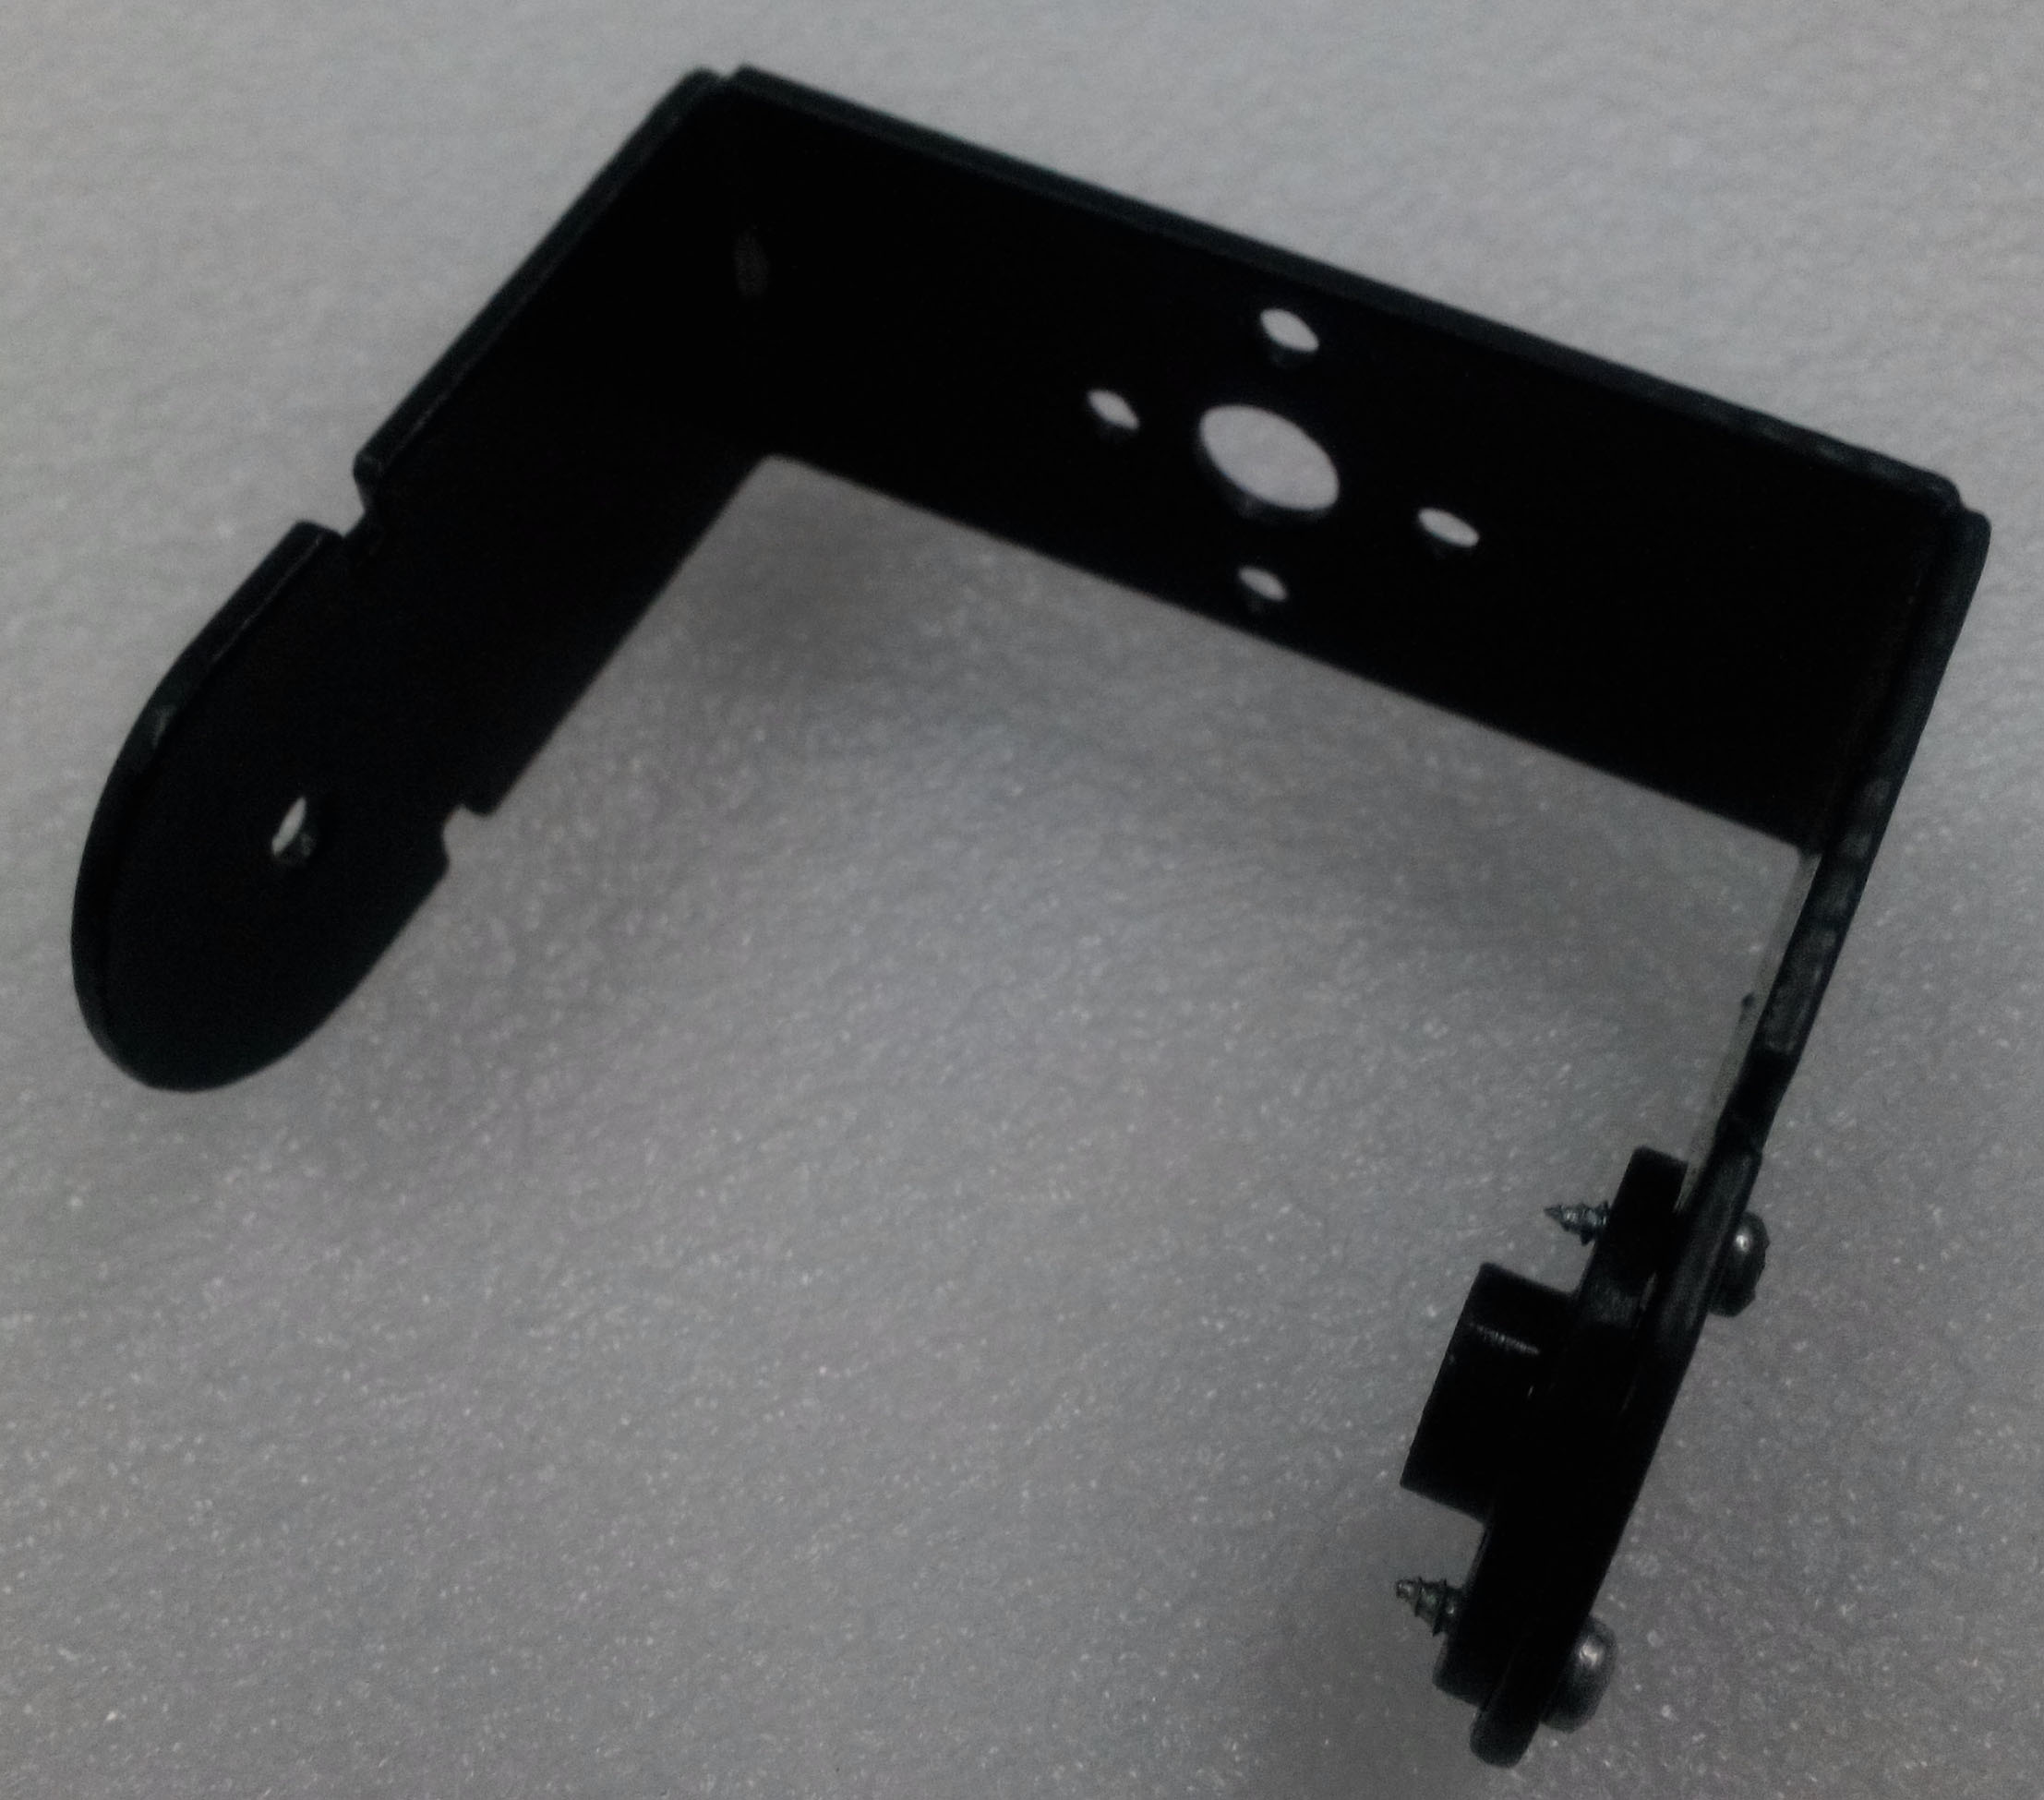
\includegraphics[width = 7cm,height= 6cm]{C_bracket_with_flap.jpg}}
	\newline
	
	\caption{Basic Linkage}
\end{figure}
\newpage
\begin{figure}[h!]
	\ContinuedFloat
	\centering
	\subfloat[Linkage of servo with C bracket]{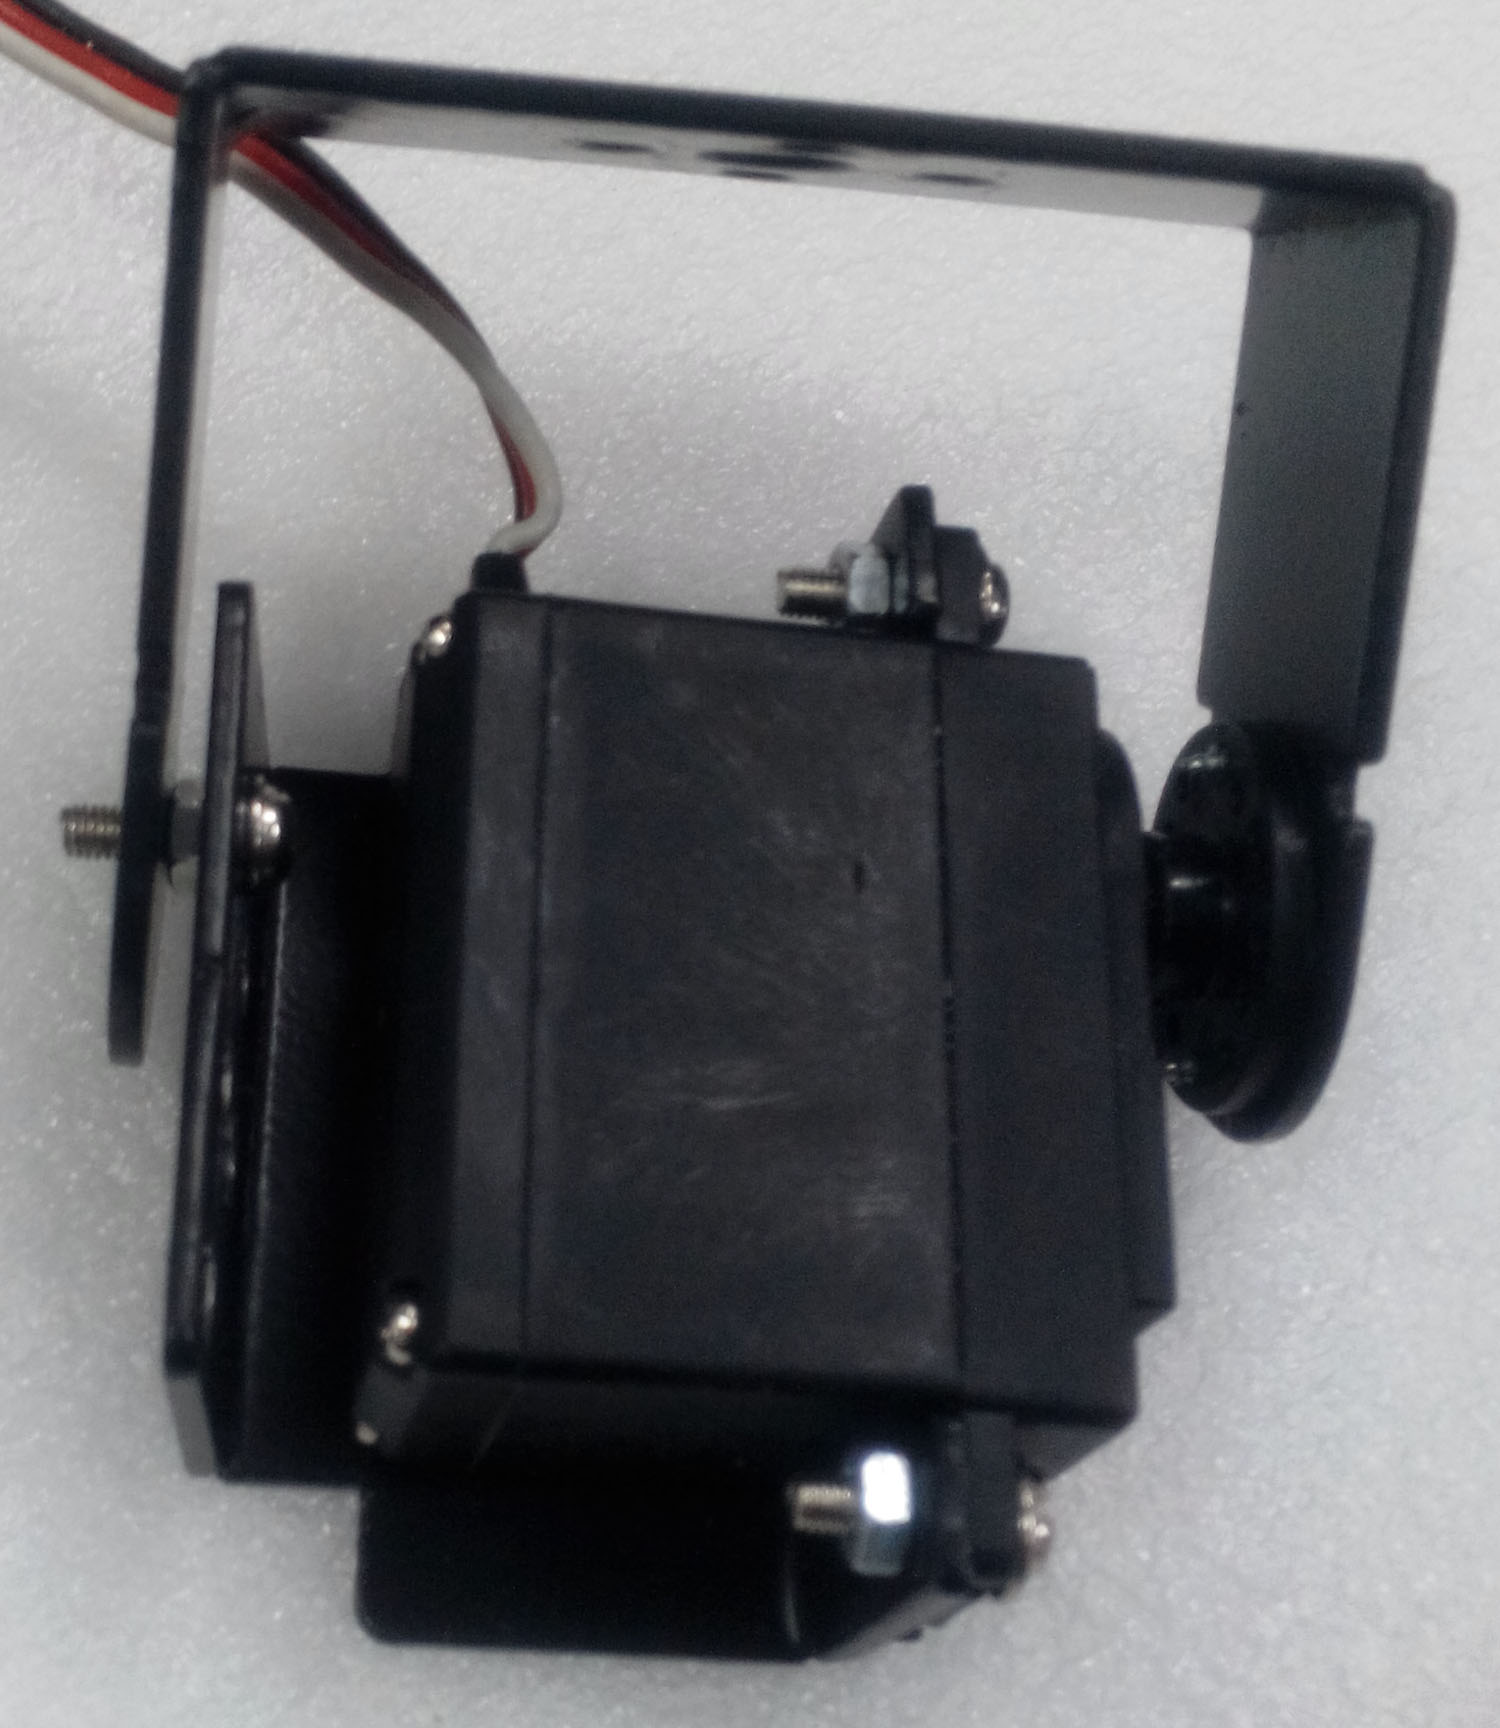
\includegraphics[width = 7cm,height= 6cm]{Servo_link.jpg}} 
	\hspace{2cm}
	\subfloat[Hip and knee linkage]{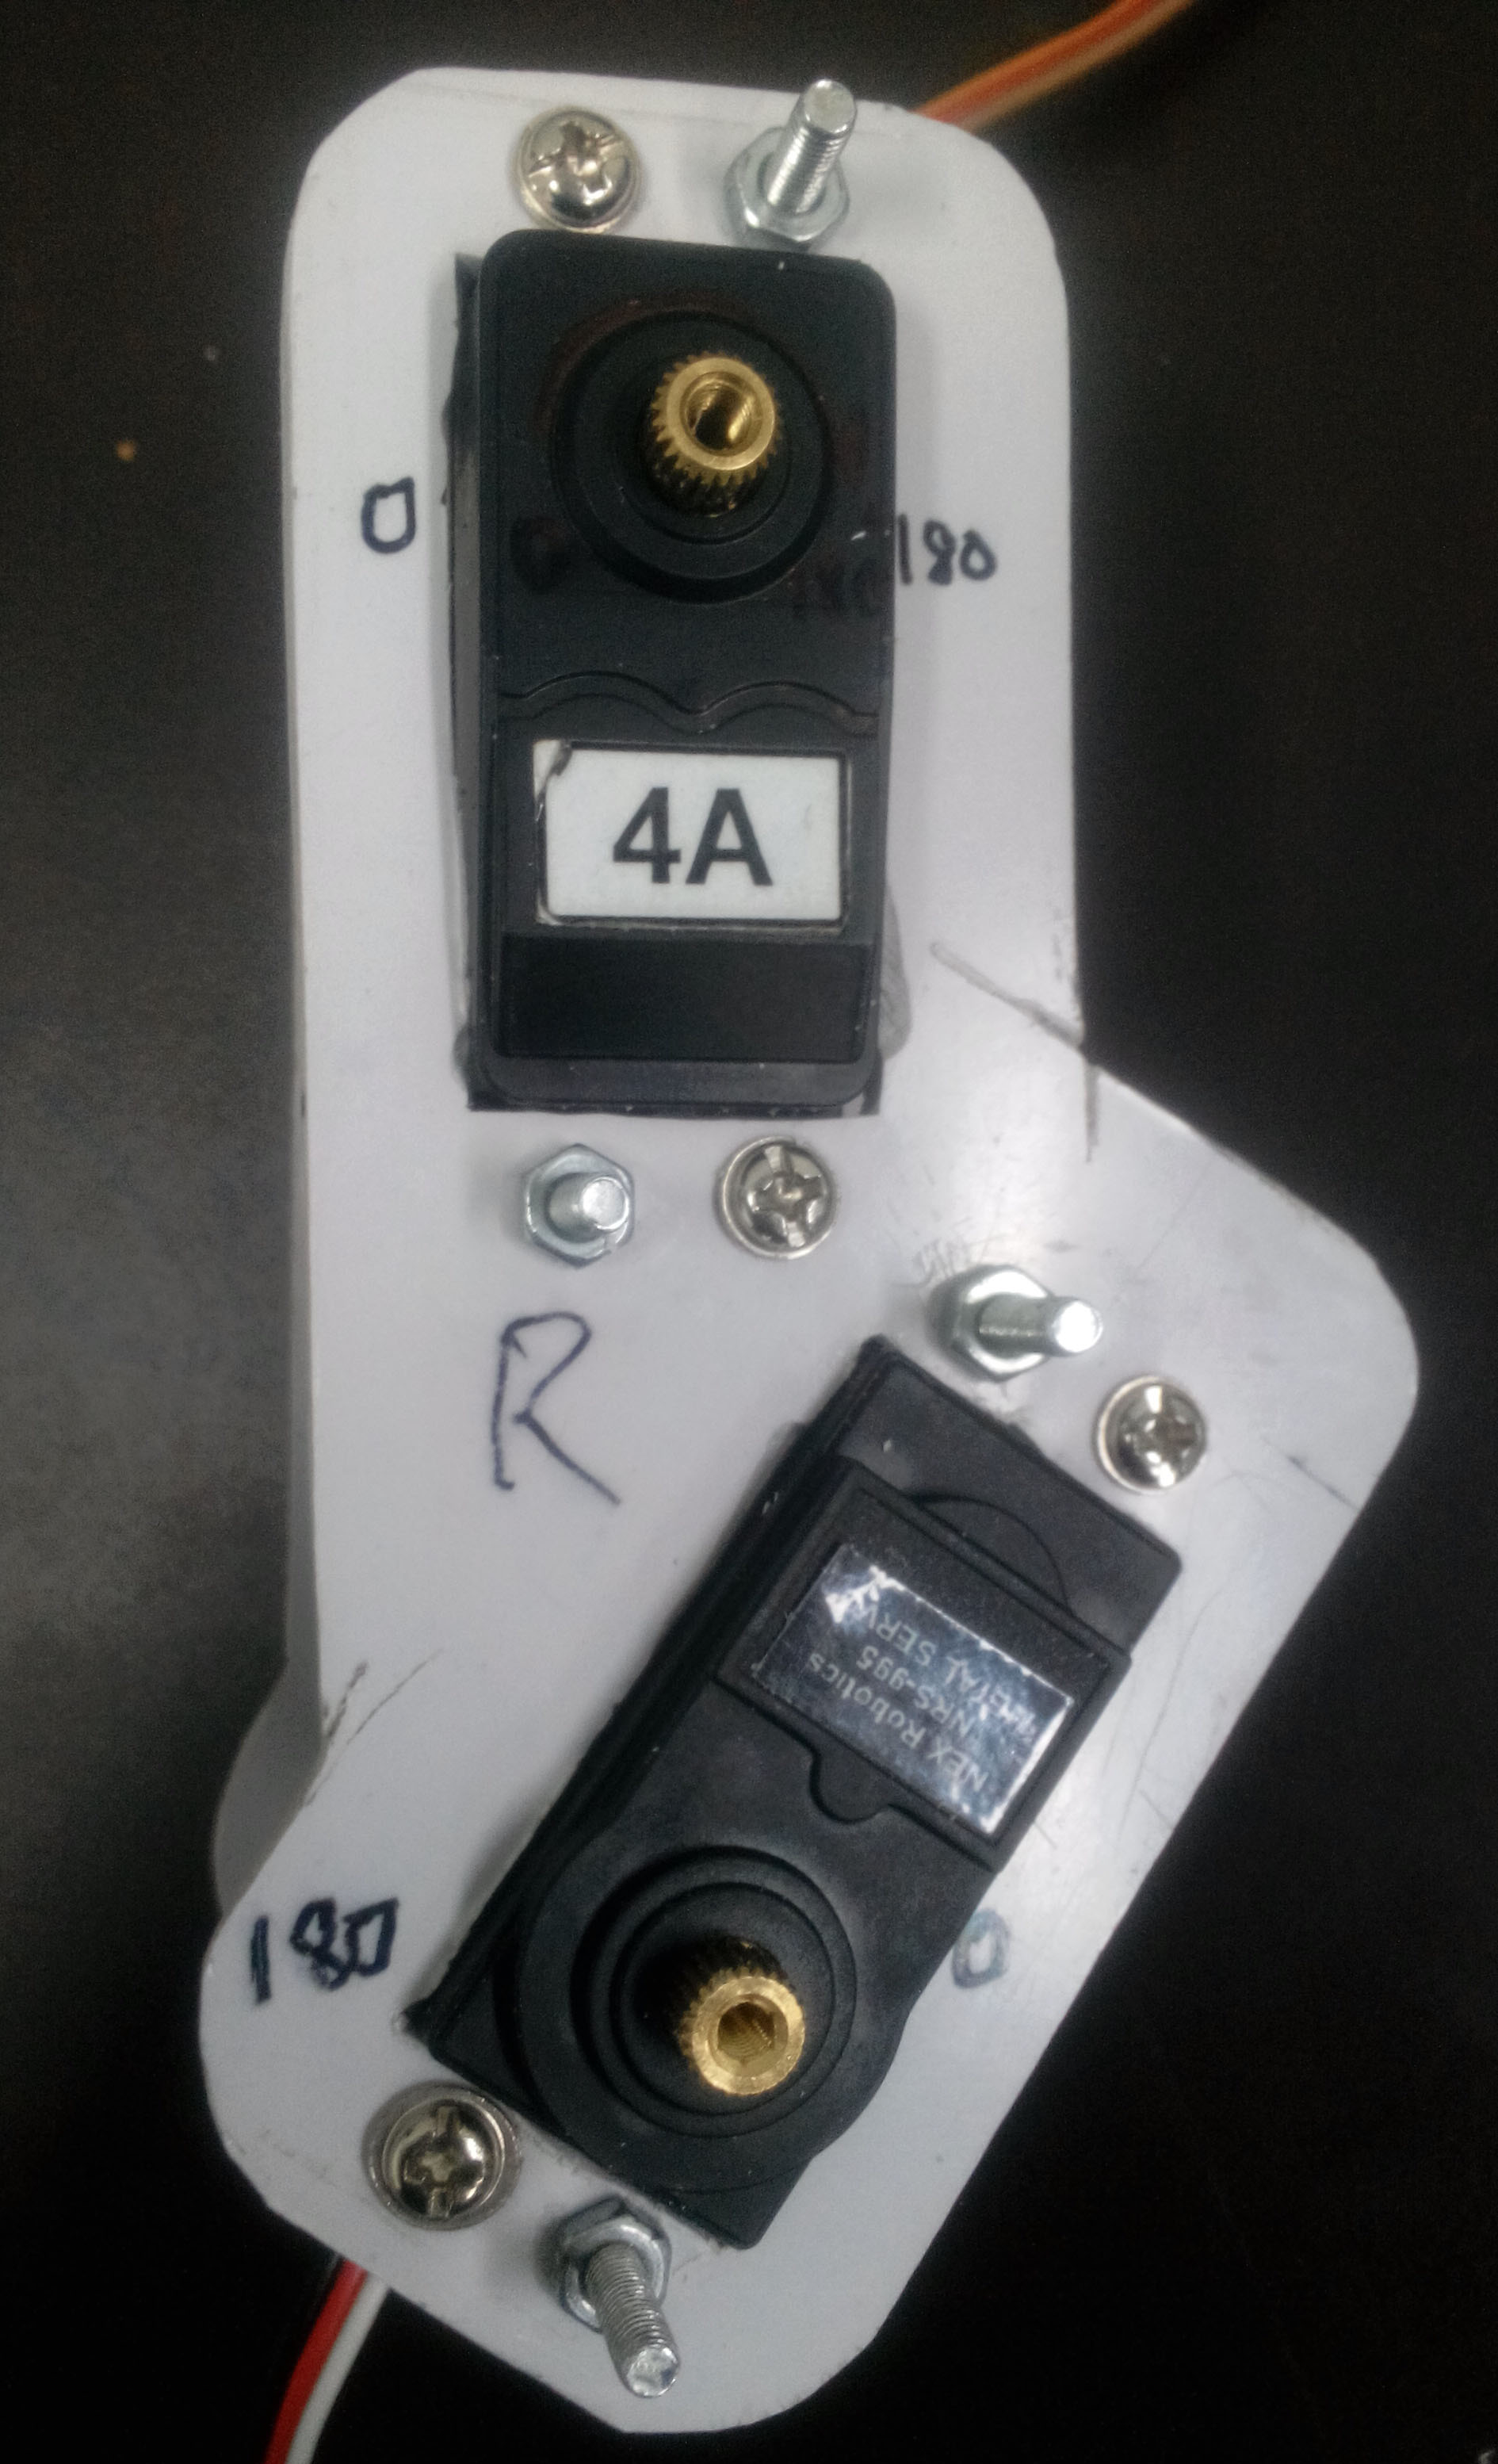
\includegraphics[width = 5cm,height= 6cm]{HipKnee.jpg}}
	\newline
	
	\caption{Basic Linkage}
\end{figure}
The construction of the robot can divided in two parts :
\begin{enumerate}
	\item Upper body
	\item Lower body
\end{enumerate}
\begin{enumerate}
\item Upper body \newline
\textbf{Torso construction} \newline
The torso represents the body of the humanoid robot to which the head, hands and
the lower body are attached. The dimensions of the torso are 11x14x7 cm. The torso
will be consisting of the heart of robot which is the processor along with the battery.
The torso is prepared using hard polymer as shown in Figure. \newline
\begin{center}
	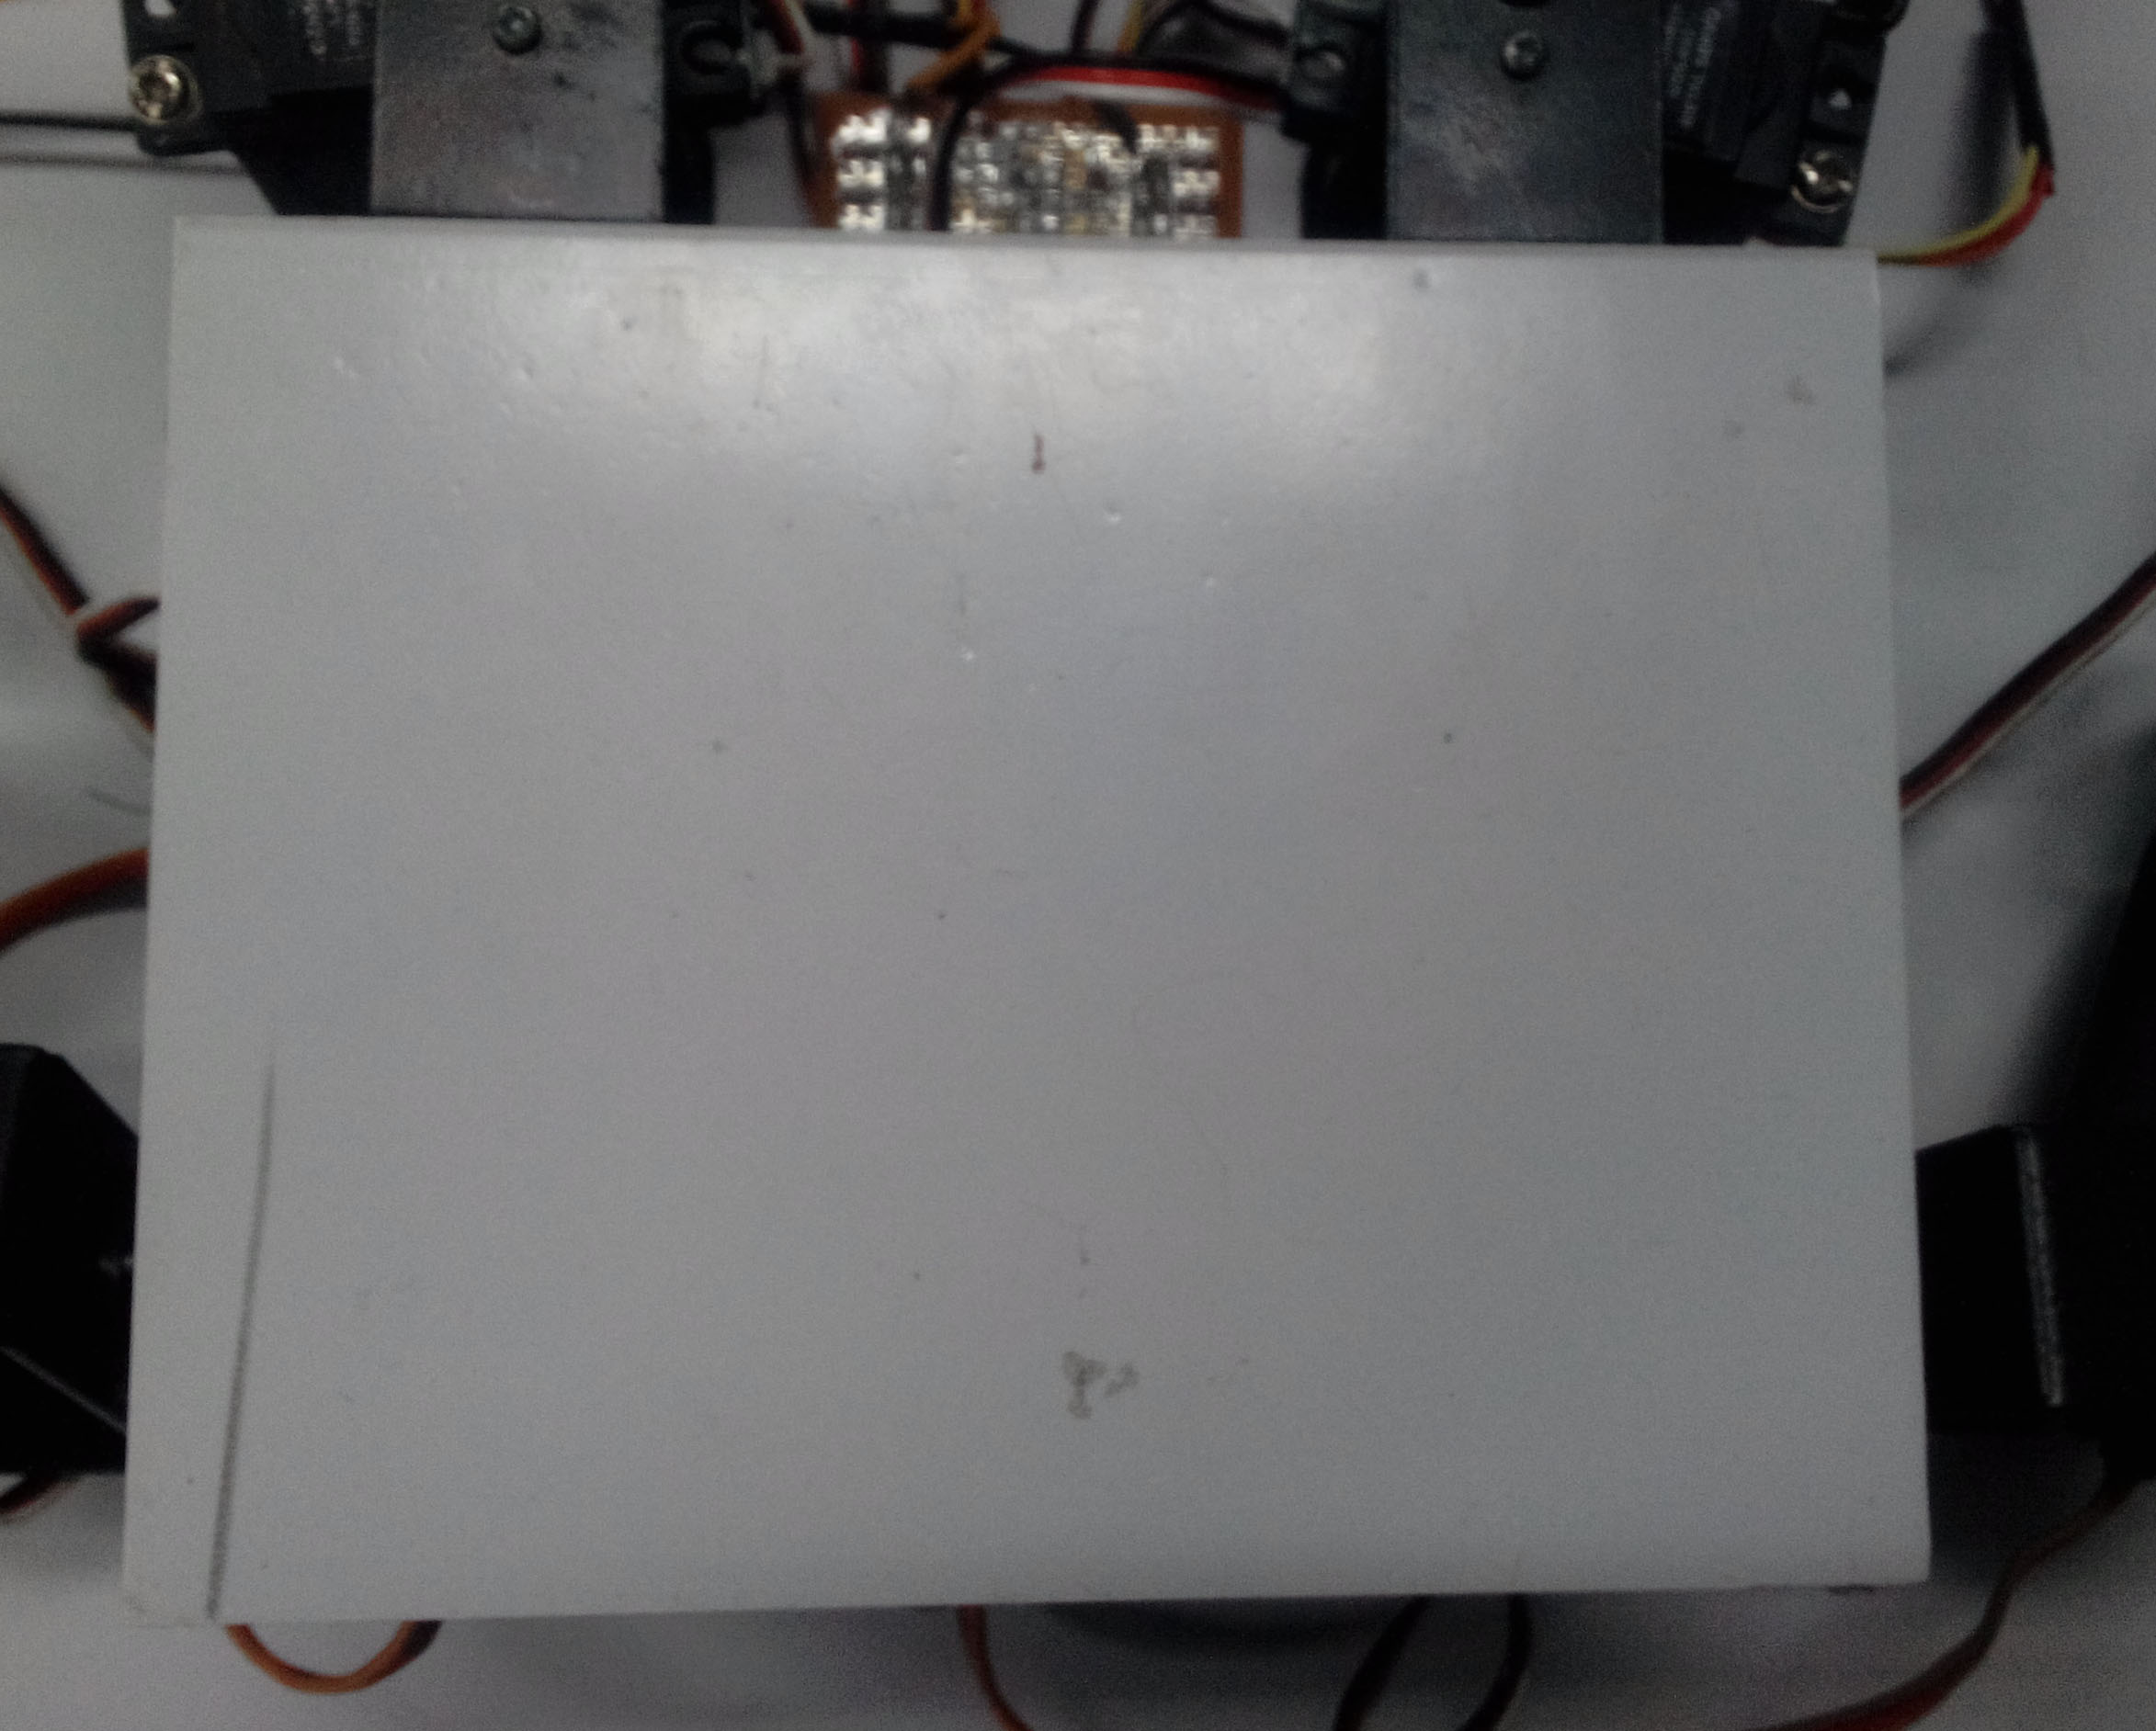
\includegraphics[width = 11cm,height= 9cm, angle =180]{torso.jpg}
\end{center}
\newpage
\textbf{Arms of the robot} \newline
By convention there are two arms of a humanoid robot i.e the right arm and the left
arm. Each Arm has 3 DOFs hence each arm is comprised of 3 servos. The
individual links are assembled together to form the desired arm joints and length.
Below is the image indicating the construction of the arm. \newline
\begin{center}
	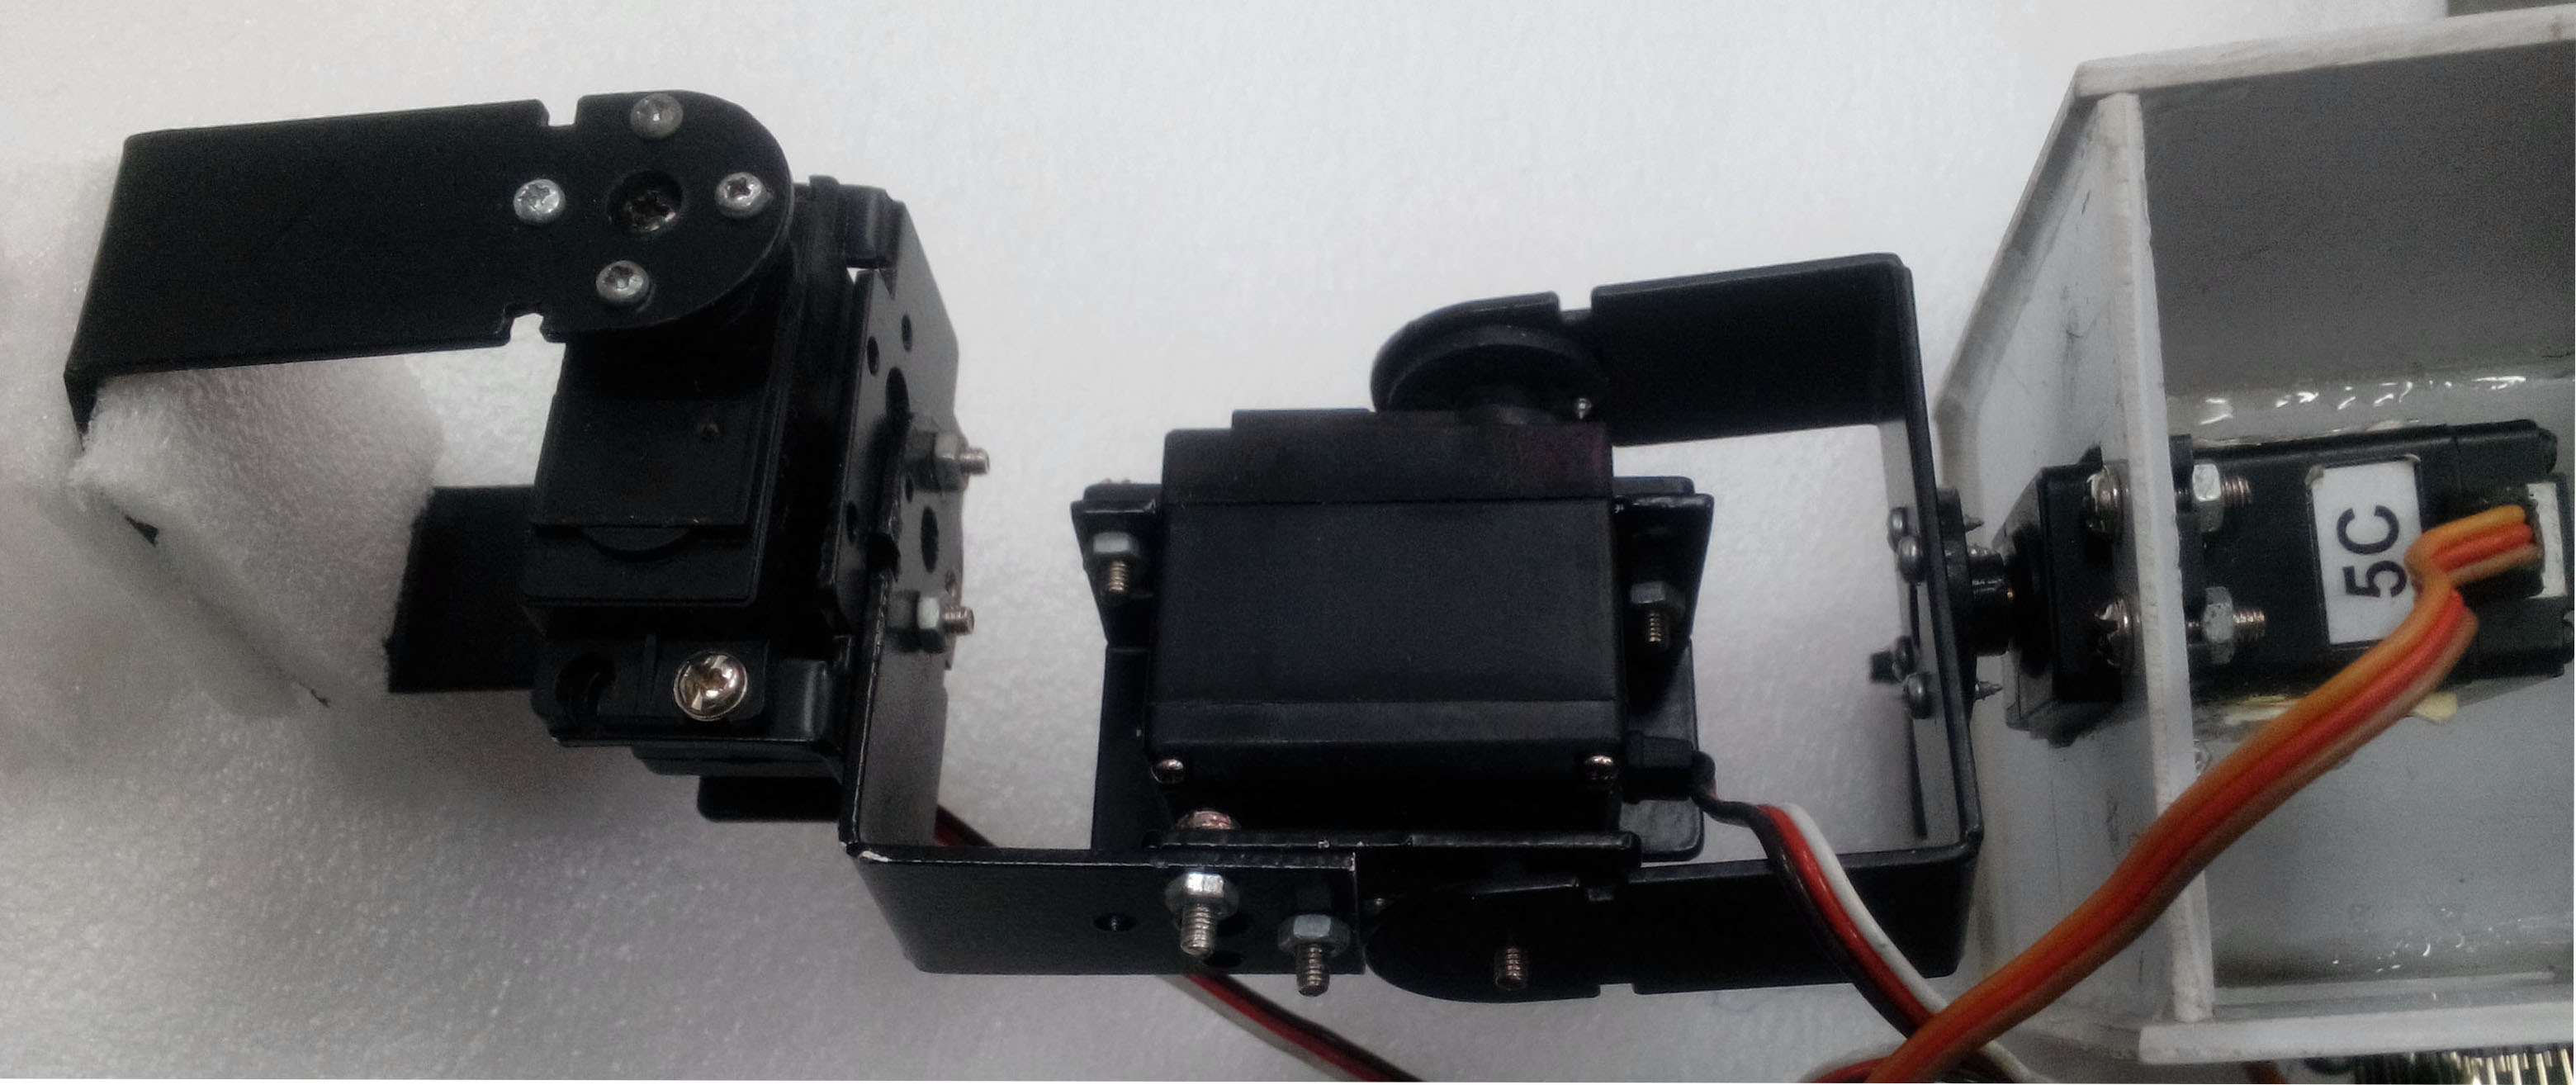
\includegraphics[width = 13cm,height= 5cm]{hand.jpg}
\end{center}

\item Lower body \newline
The lower basically has the two legs which are required for the locomotion of the
humanoid robot. The basic servo links and the Hip Knee linkage is used to form the
leg for the robot. Each leg has 5 DOFs hence each leg is comprised of 5 servos. The
below image gives an idea about the various joints in the leg.

\begin{center}
	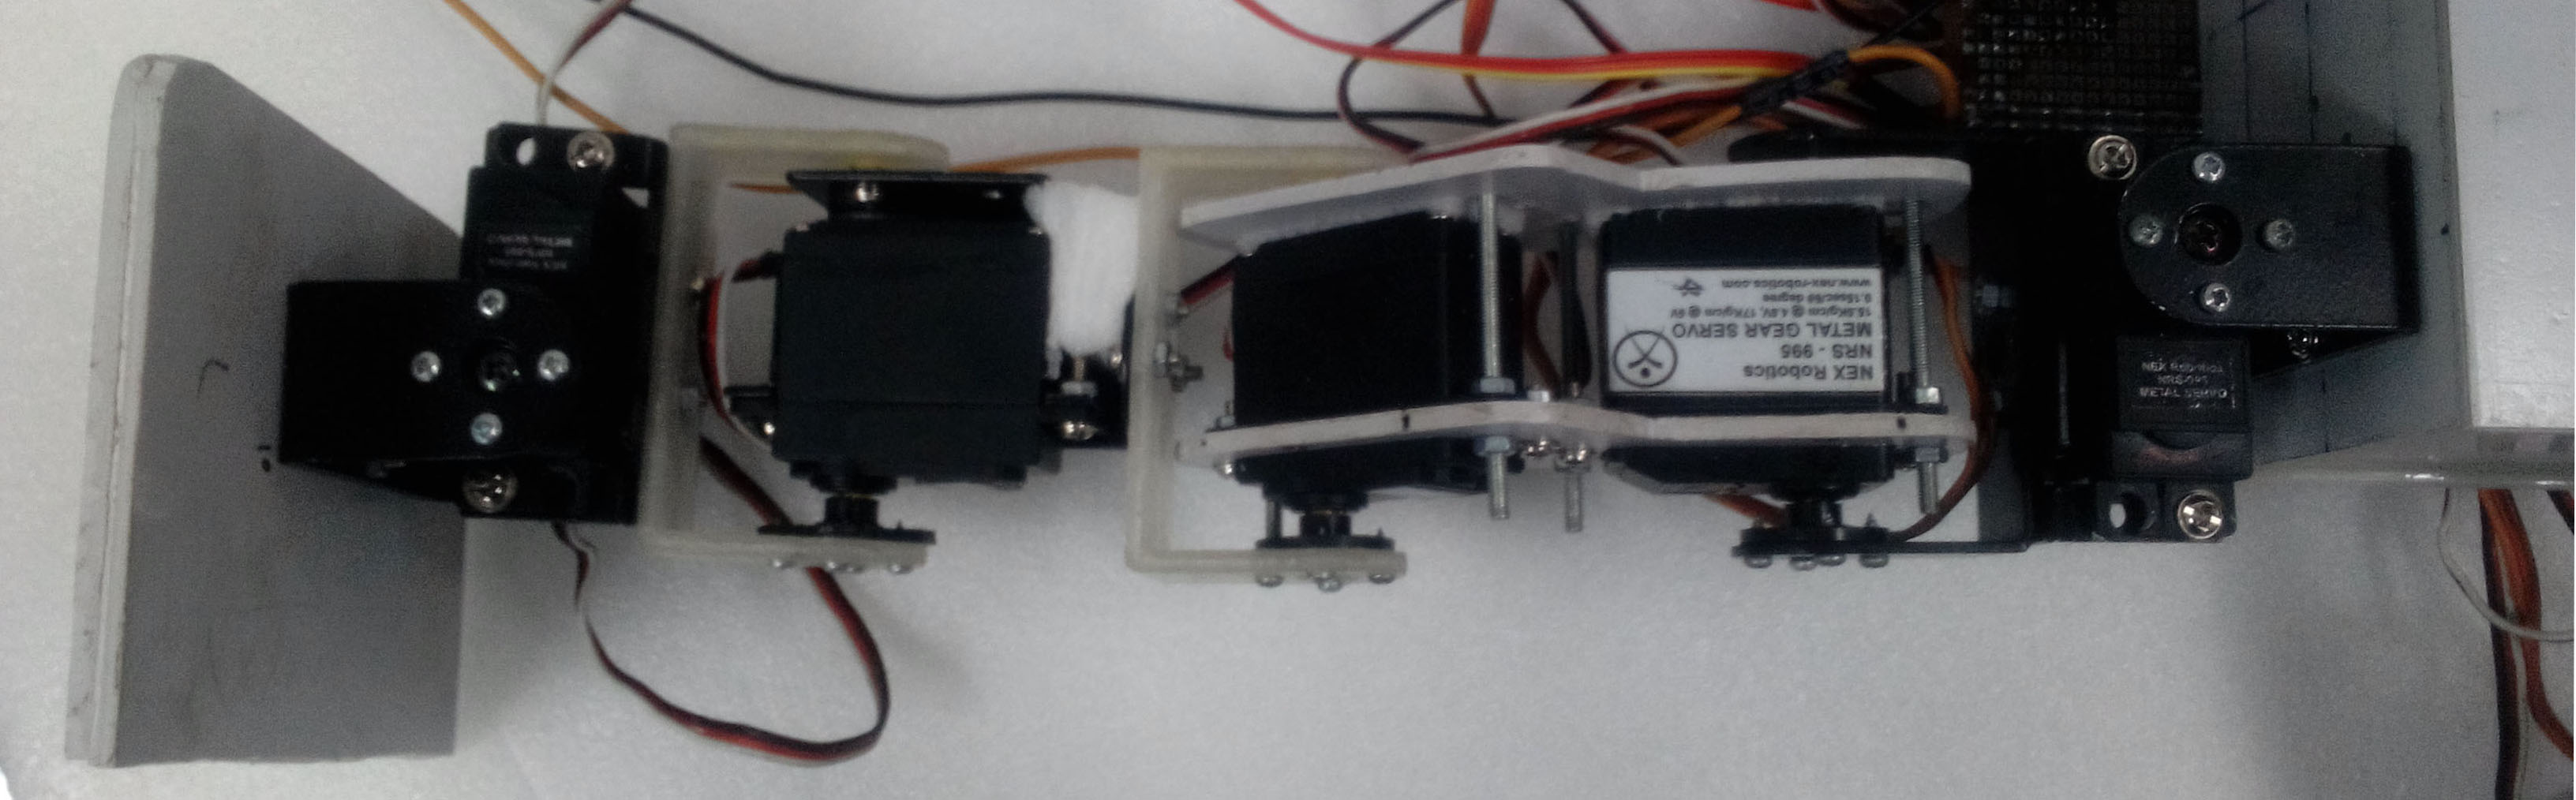
\includegraphics[width = 13cm,height= 5cm]{leg_fv.jpg}\\{Leg front view} \\
	\vspace{1cm}
	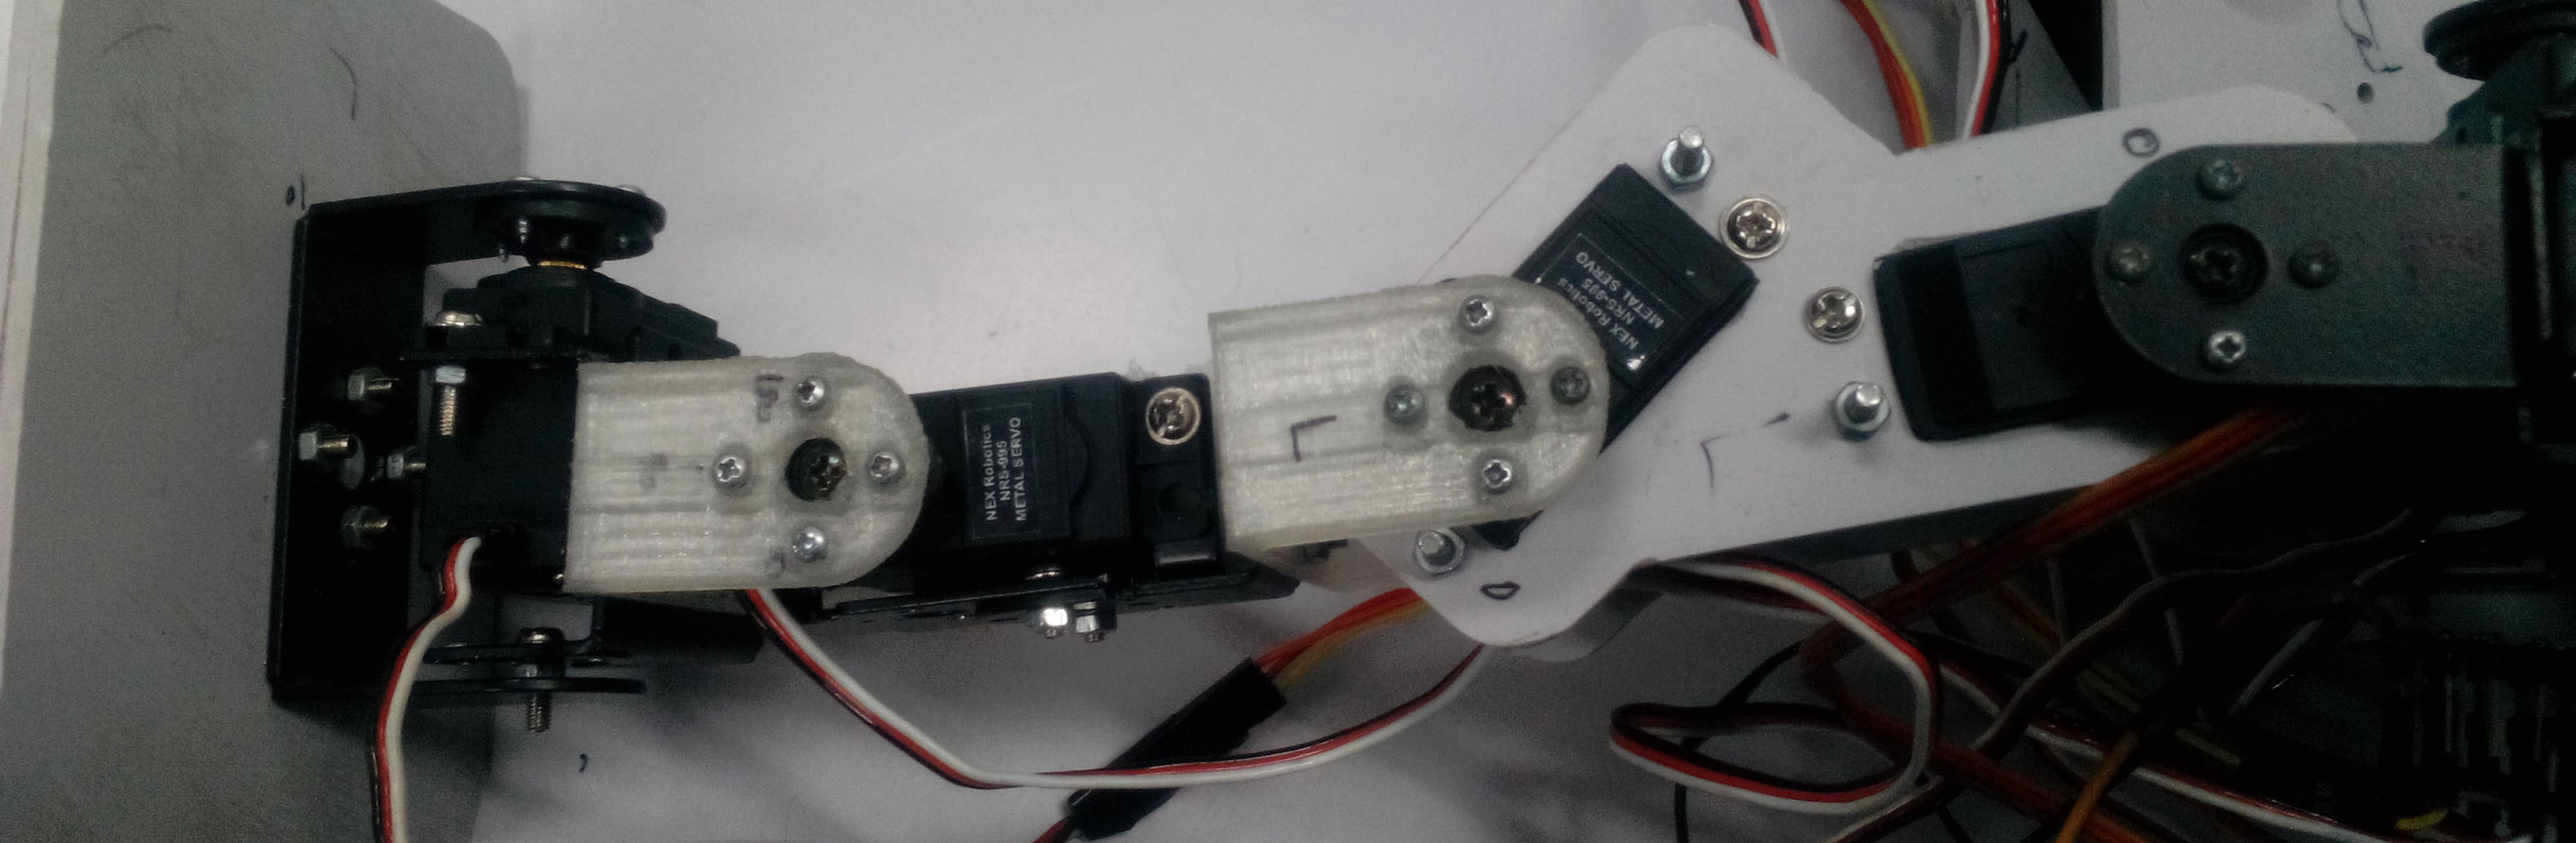
\includegraphics[width = 13cm,height= 5cm]{leg_SV.jpg}\\{Leg side view}
\end{center}
\end{enumerate}
\newpage
After the construction of these main parts we are now ready to assemble these body
parts as a whole to form the Humanoid robot. Below are Images of some joints and
the final assembly of the Robot.
\begin{figure}[h!]
	\centering
	\subfloat[Shoulder link]{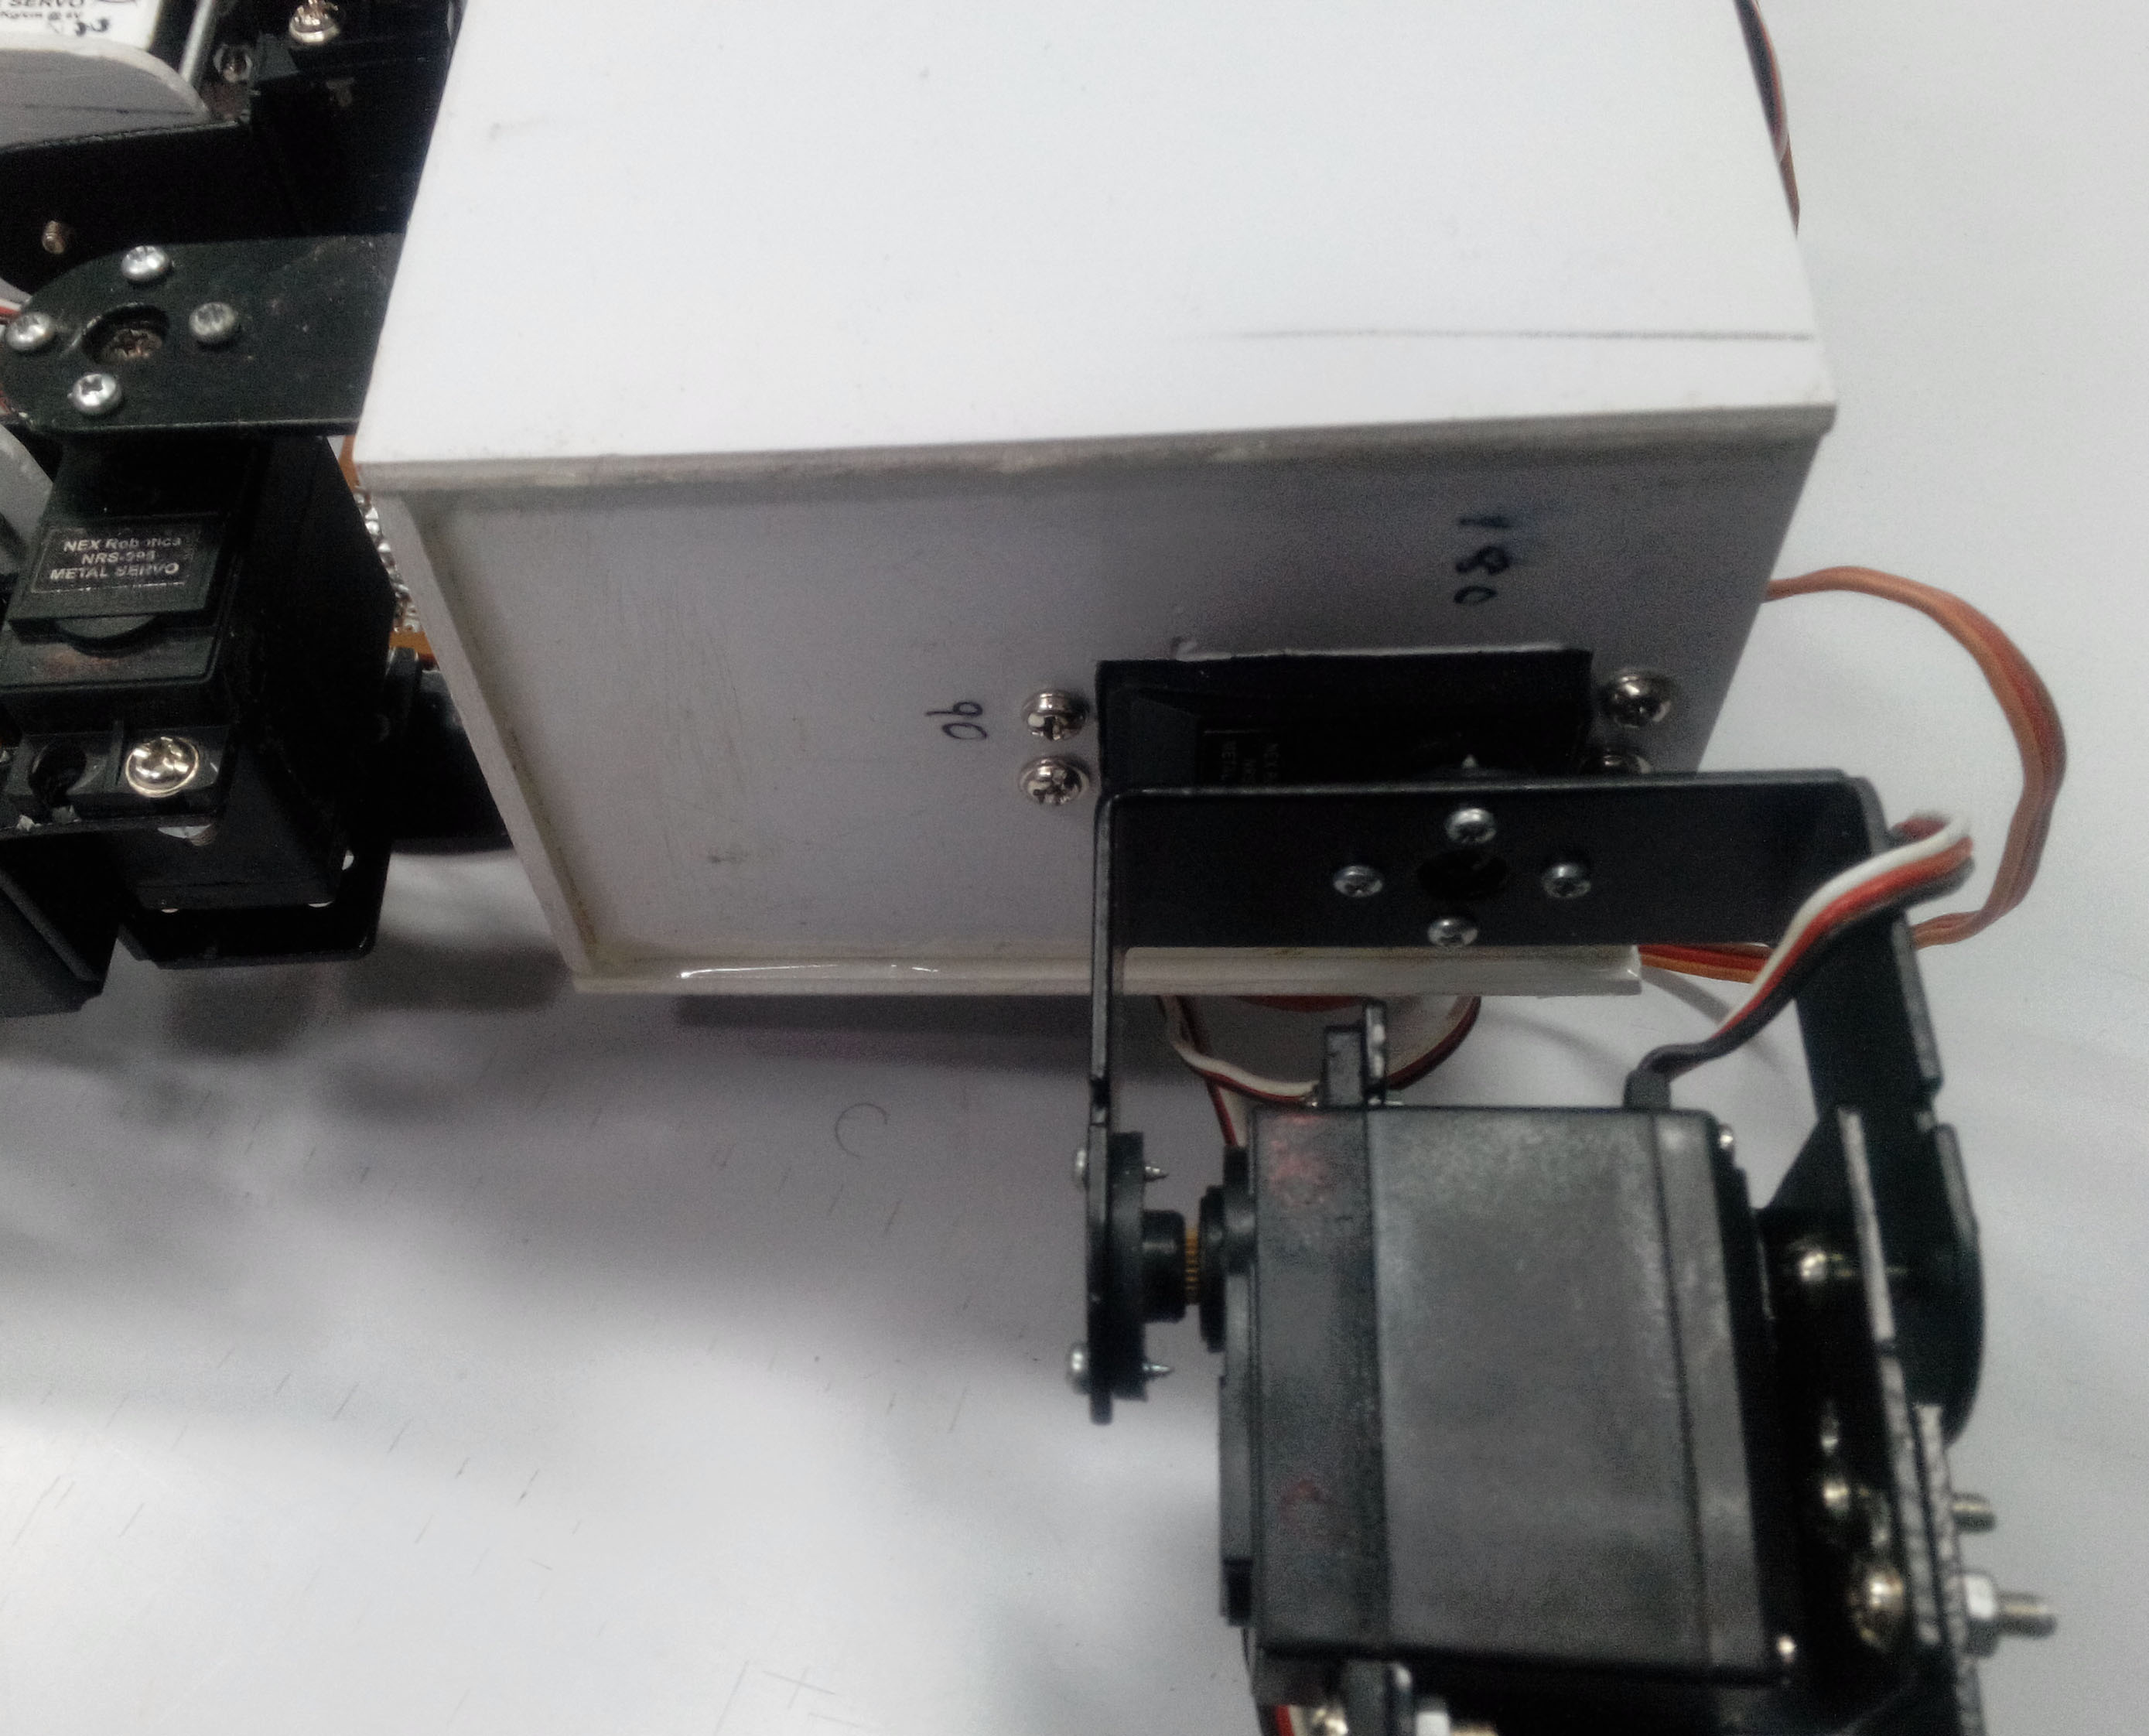
\includegraphics[width = 7.5cm,height= 9cm]{shoulderlink.jpg}} 
	\hspace{1cm}
	\subfloat[Foot link]{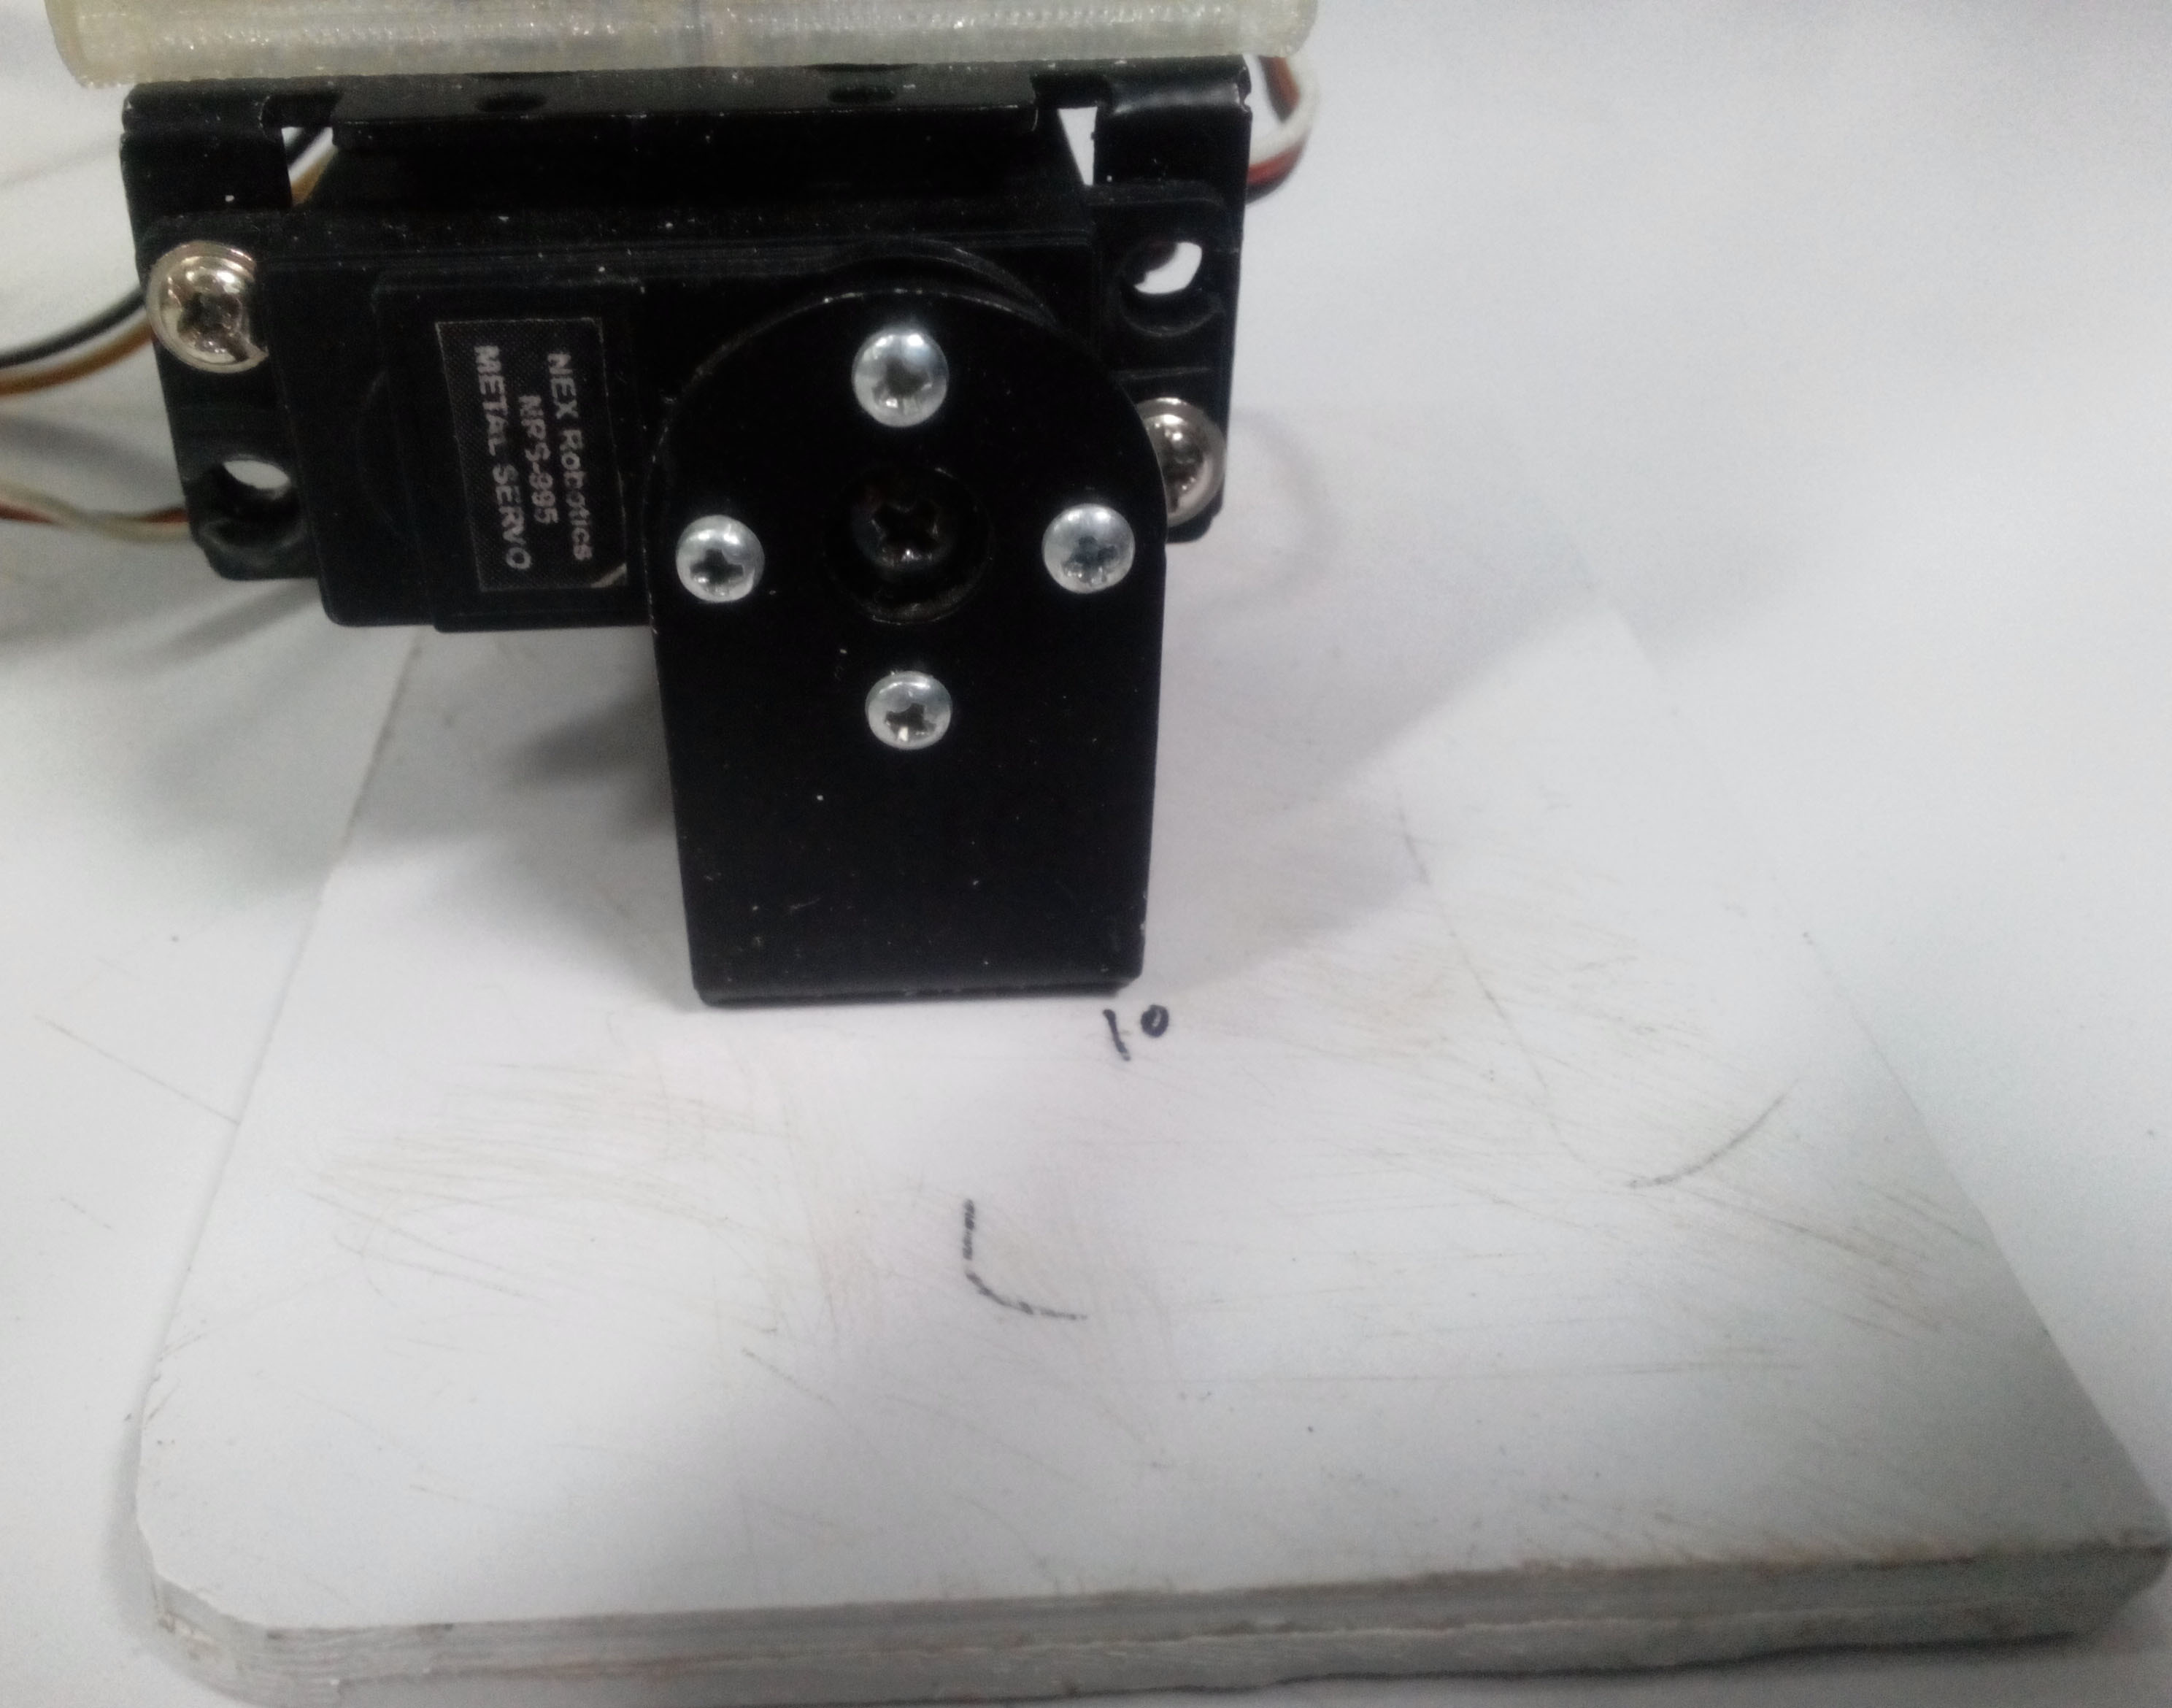
\includegraphics[width = 7.5cm,height= 9cm]{foot.jpg}}
	\newline
	\subfloat[Hip link]{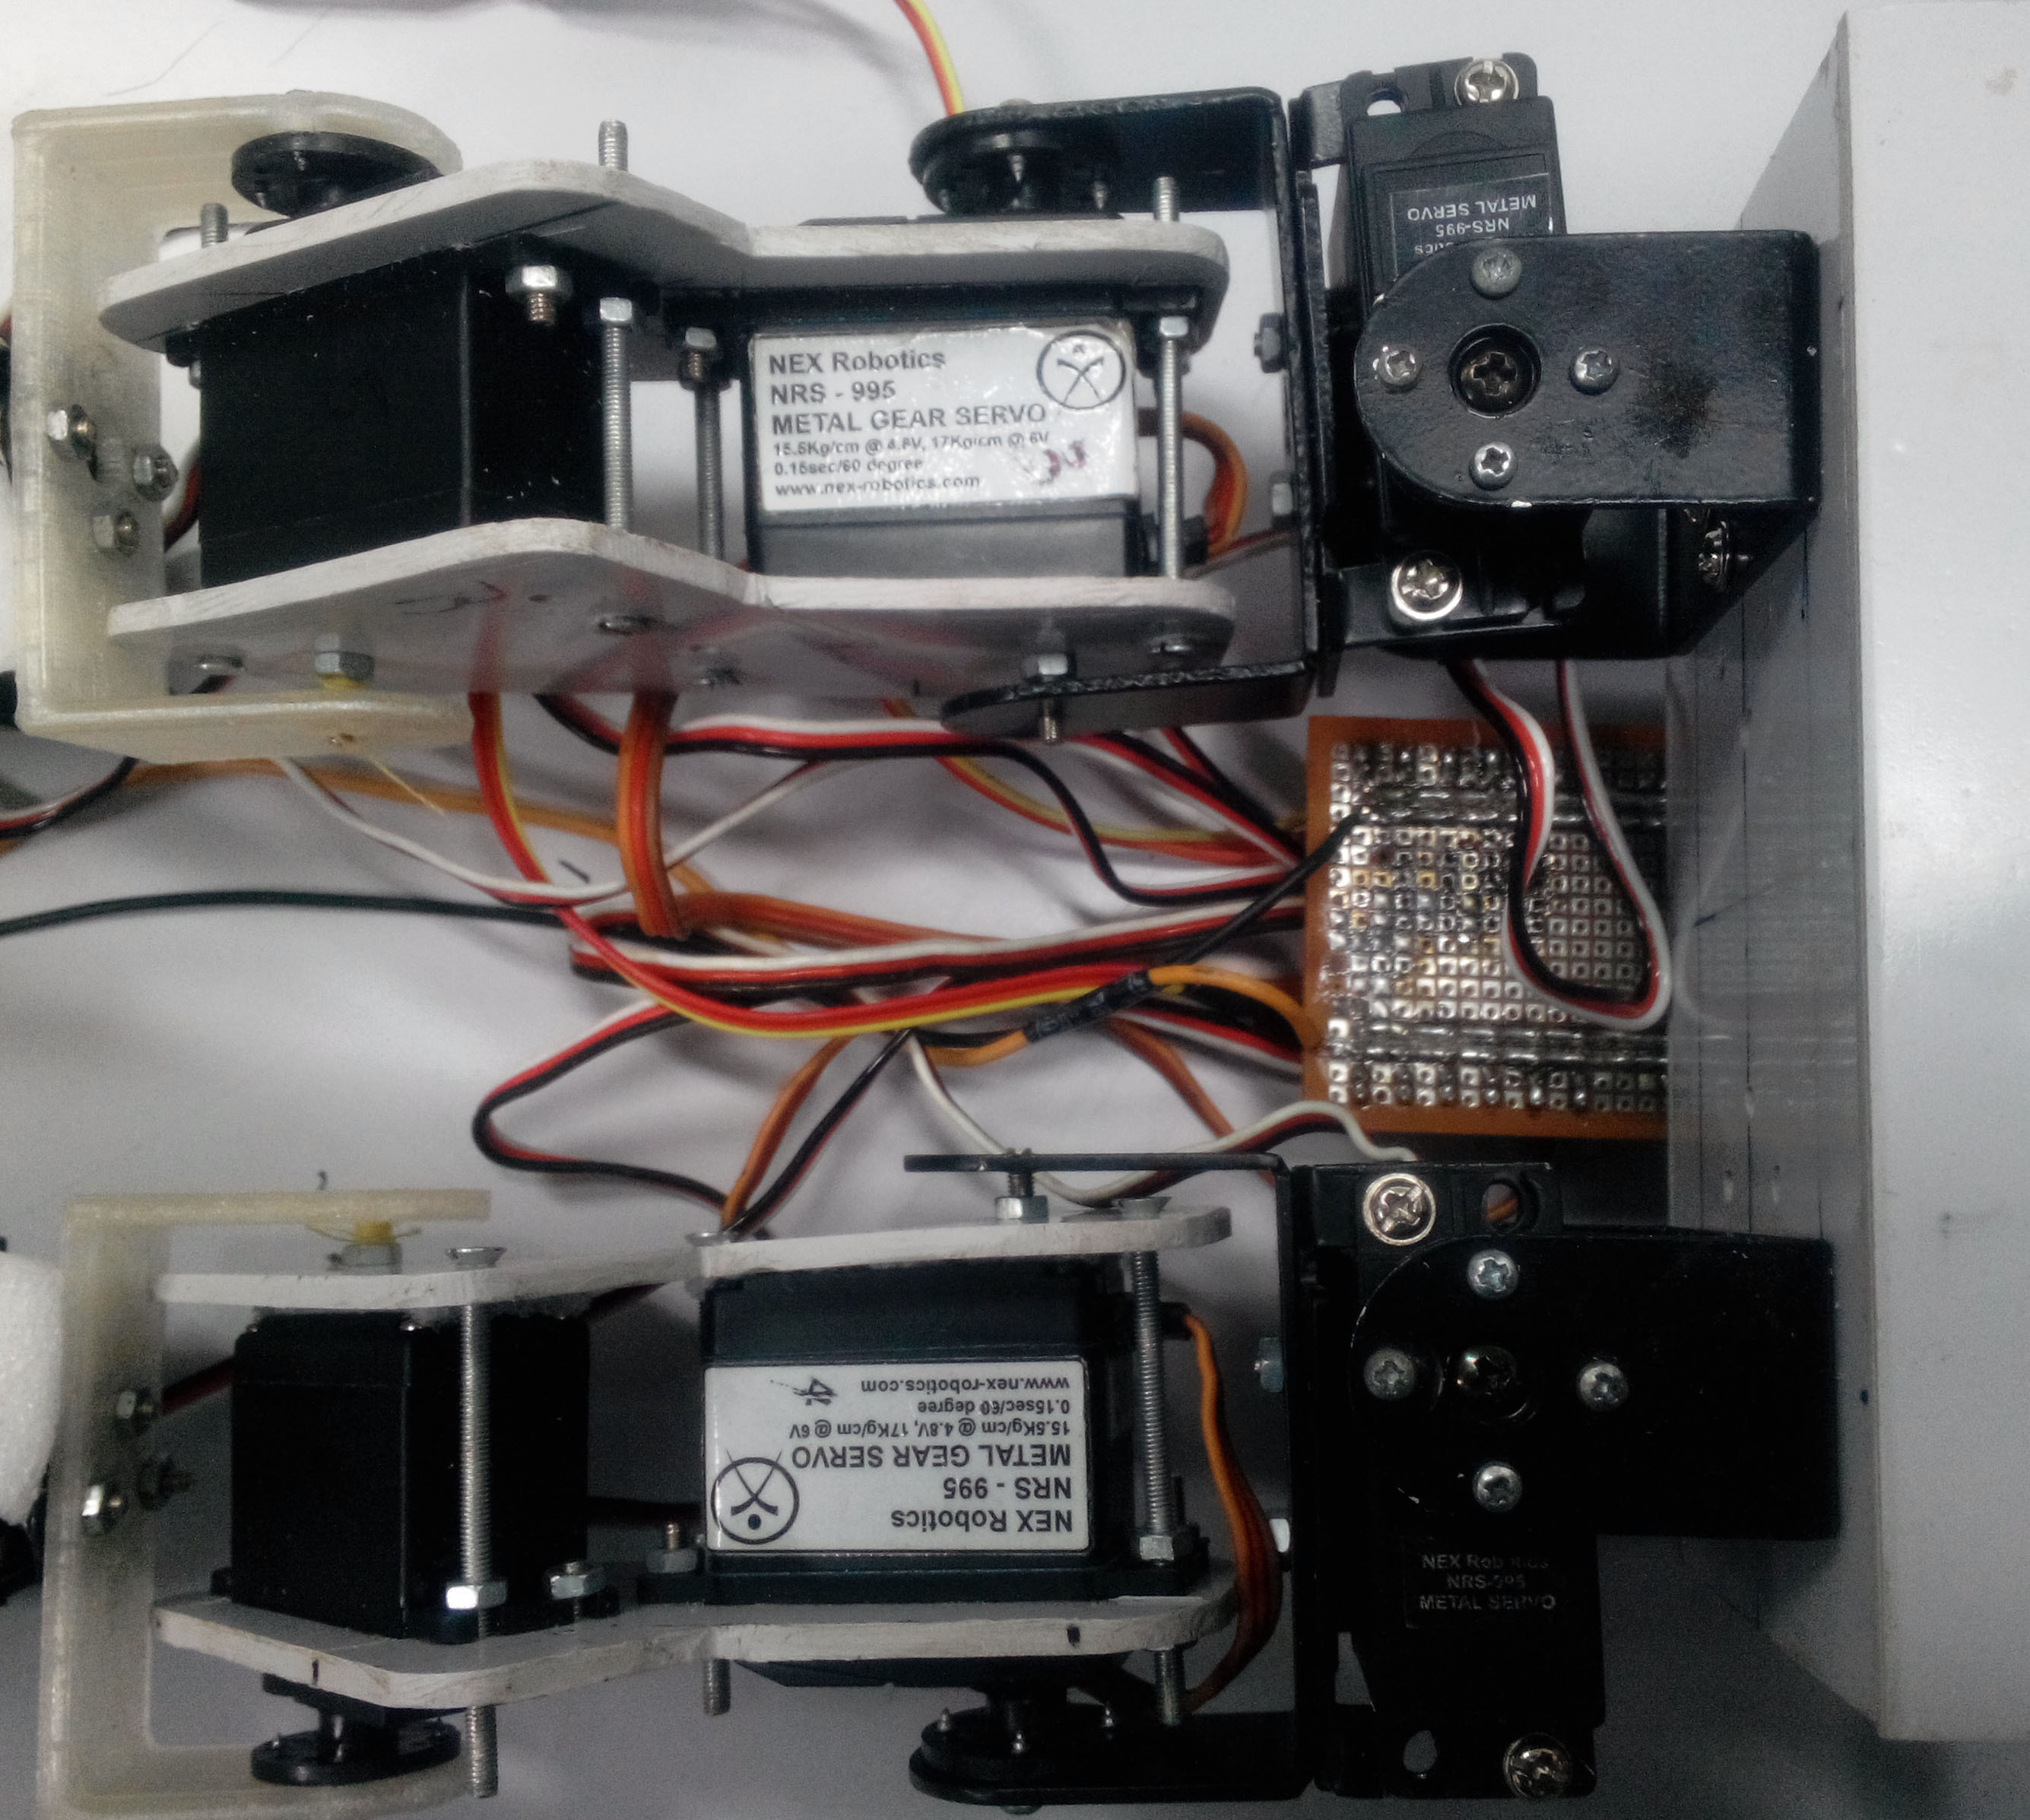
\includegraphics[width = 10cm,height= 9cm]{hip_torso_linkage.jpg}}
	\caption{Final Assembly}
\end{figure}
\newpage
\begin{figure}[h!]
	\ContinuedFloat
	\centering
	\subfloat[Final assembly of the robot]{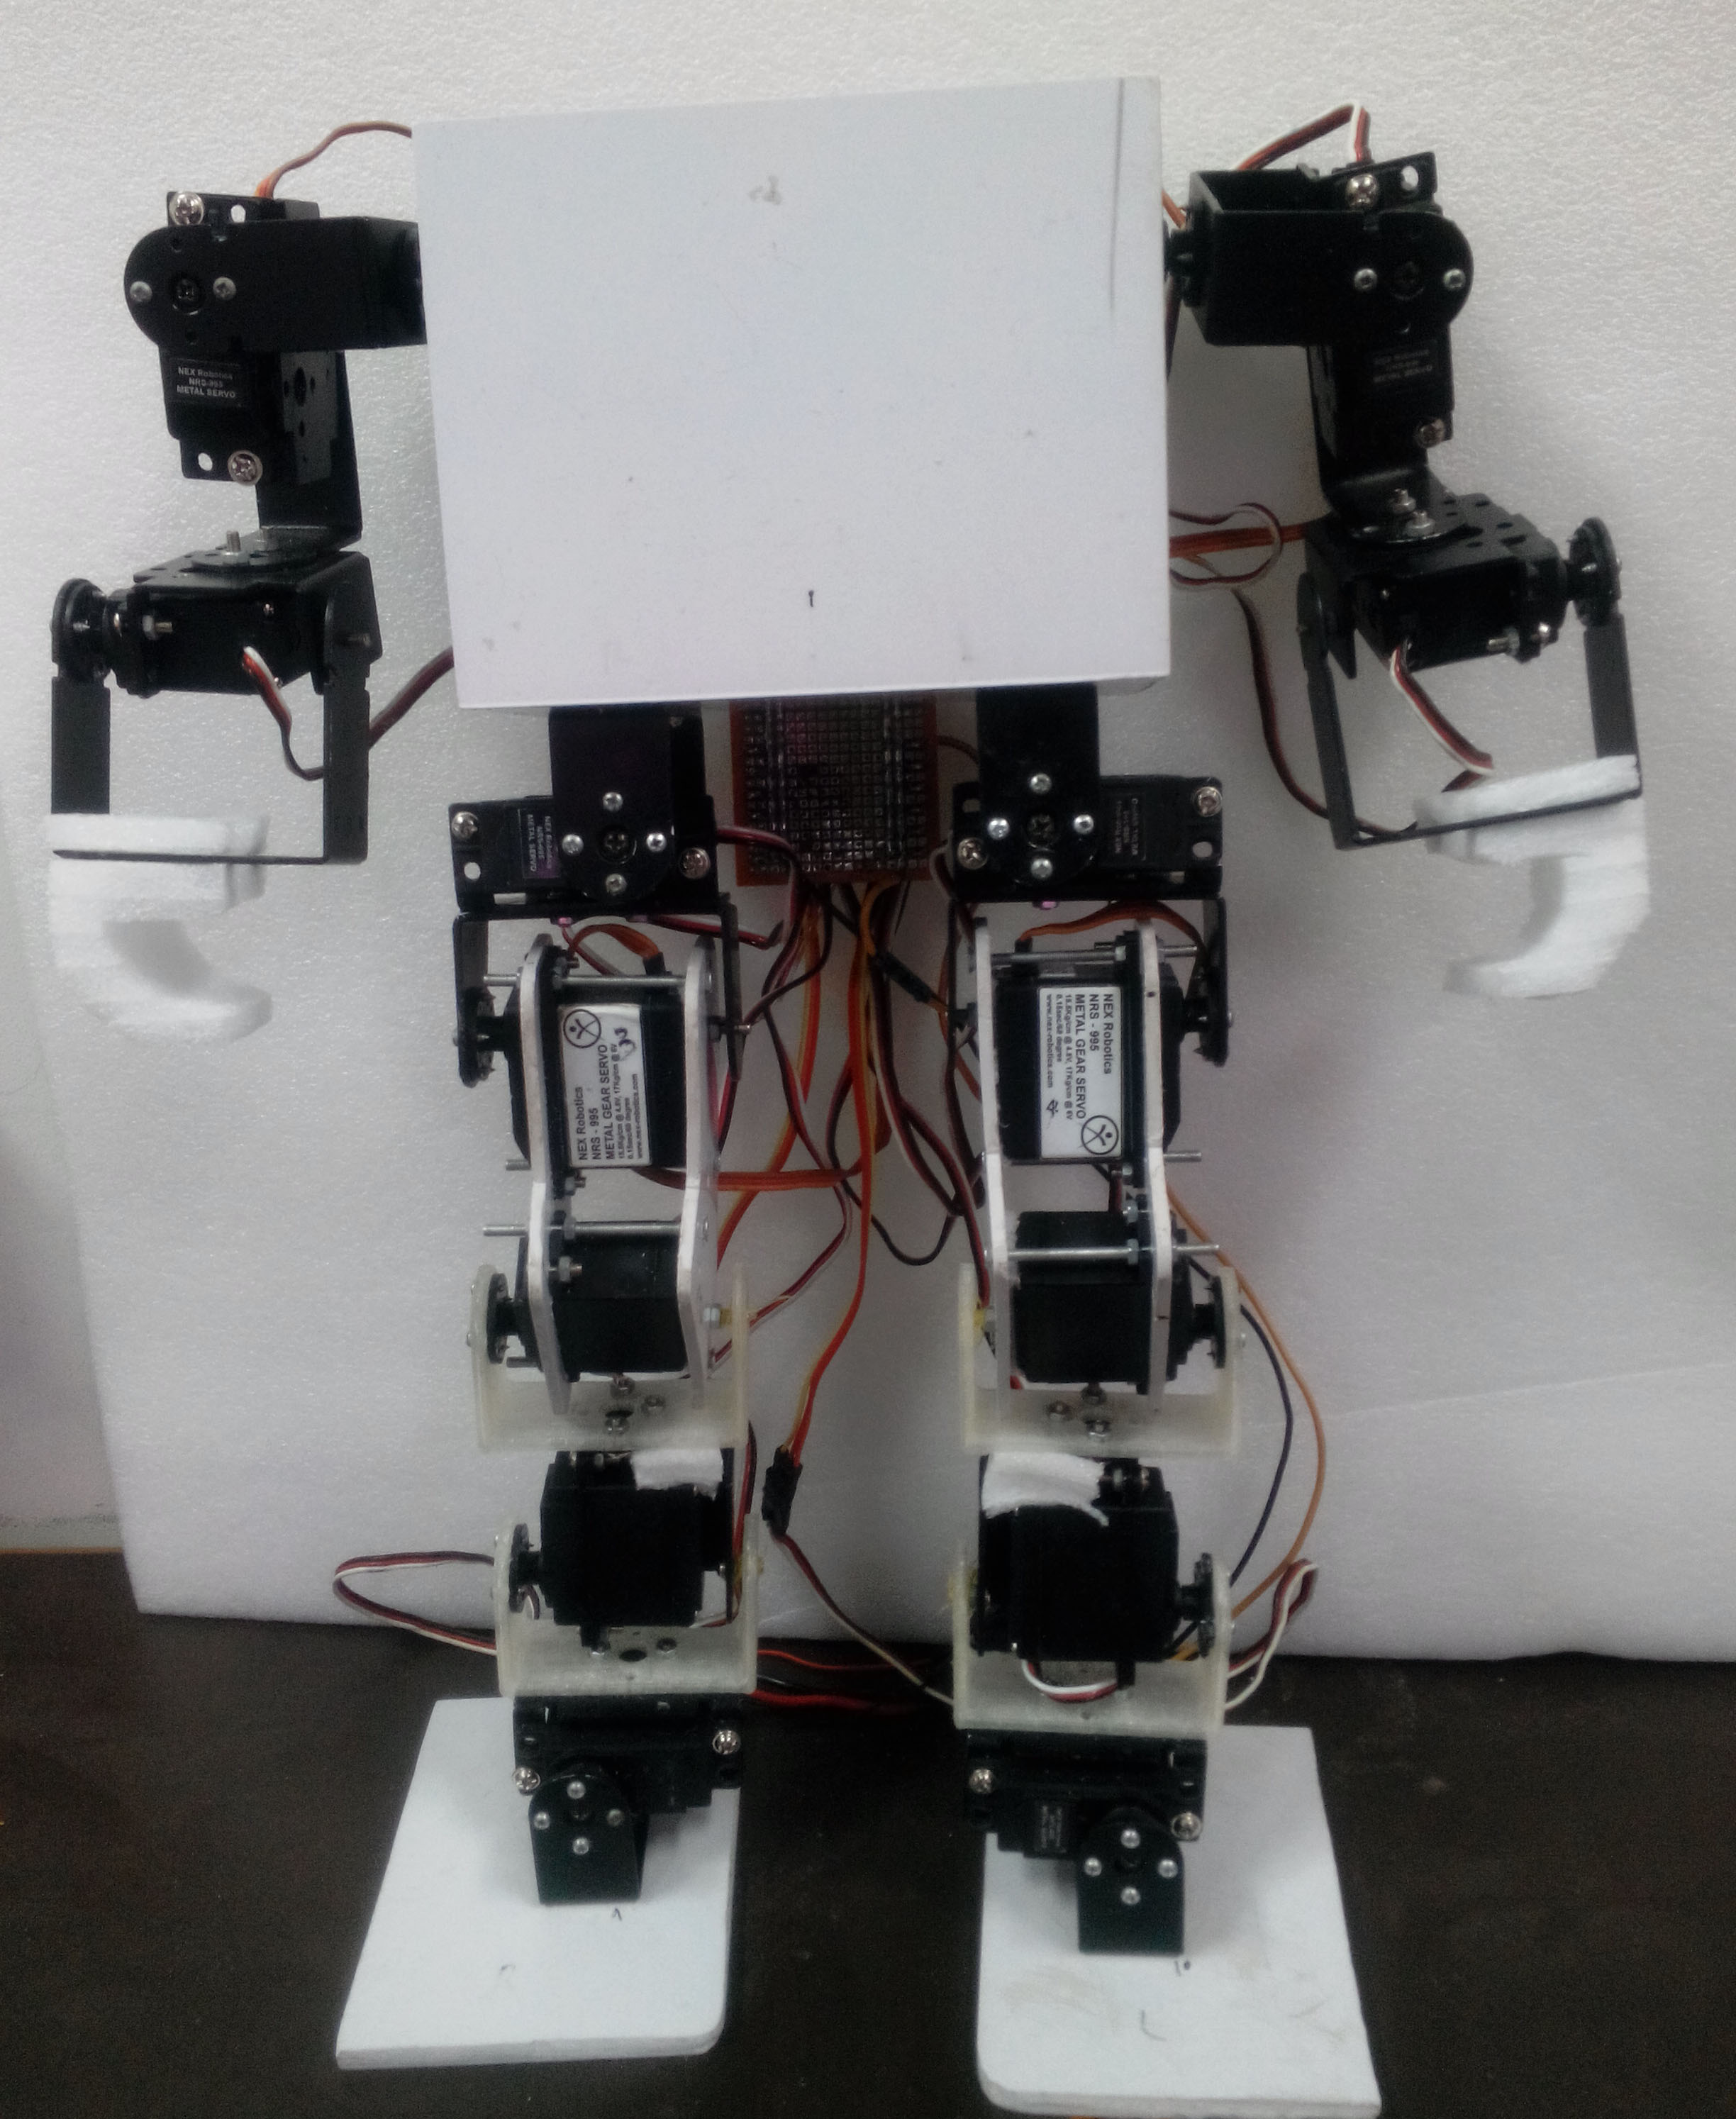
\includegraphics[width = 7.5cm,height= 11cm]{body_assembly.jpg}} 
	\hspace{1cm}
	\subfloat[servo numbering]{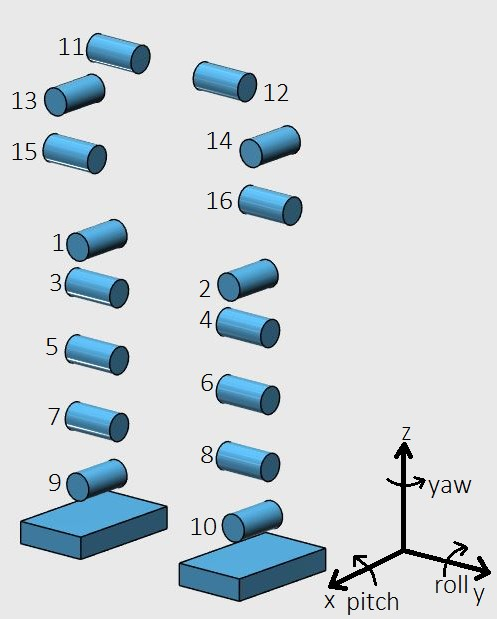
\includegraphics[width = 7.5cm,height= 11cm]{servo_num.jpg}}	
	\caption{Final Assembly}
\end{figure}

\begin{table}[h!]
	\centering
	\begin{tabular}{ |l|c|c|c| } 
		\hline
		Right leg & & Left leg &  \\
		\hline
	Upper hip & Servo 1 & Upper hip & Servo 2\\
	Lower hip & Servo 3 & Lower hip & Servo 4\\
	Knee & Servo 5 & Knee & Servo 6\\
	Upper ankle & Servo 7 & Upper ankle & Servo 8\\
	Lower ankle & Servo 9 & Lower ankle & Servo 10\\
	\hline
	Right Arm  & & Left Arm &\\
	\hline
	Inner shoulder & Servo 11 & Inner shoulder & Servo 12\\
	Outer shoulder & Servo 13 & Outer shoulder & Servo 14\\
	Elbow & Servo 15 & Elbow & Servo 16\\
		\hline
		
		
	\end{tabular}
	\caption{Servo Naming and their designations used in the coding}
	\label{tab2: Servo_num}
\end{table}
\newpage

\section{Motion of the Robot}
The motion of the robot is explained separately for the new design prepared in Phase 2 and
the modified new design prepared in Phase 3.
\subsection{Motion of the Phase 2 structure}
The motion of the robot was categorized in three phases which are
\begin{enumerate}
	\item Basic swing
	\item Basic knee swing
	\item Walking
\end{enumerate}
\textbf{Basic swing:} This motion can be described as the swing of the robot sideways with
both feet in contact with the ground, the center of gravity shifts towards the side where
the robot swing, for example if the bot swing towards right the CG shifts right. This
motion is carried out with help of four servos, two upper hip servos (since total of four
hip servo are present on robot we differentiate by naming them as upper and lower hip
servos) and two ankle servos. The angle traversed by the servos can be calculated by
knowing the total displacement of the CG from the initial point to final point, the
distance of CG from the ground is known then using simple trigonometry the required
angle can be calculated as shown in Fig \ref{fig:p2motion}
\begin{figure}[h!]
	
	\centering
	\subfloat{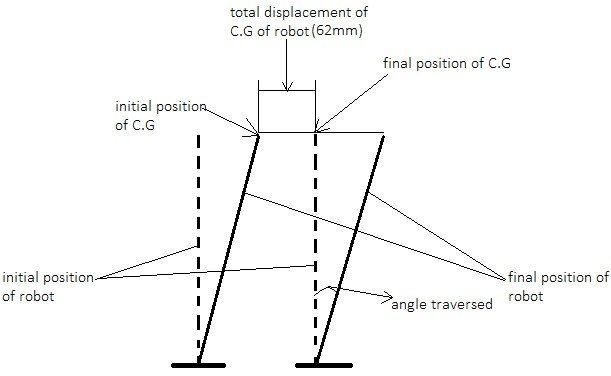
\includegraphics[width = 6cm,height= 7cm]{motion1.jpg}} 
	\hspace{2cm}
	\subfloat{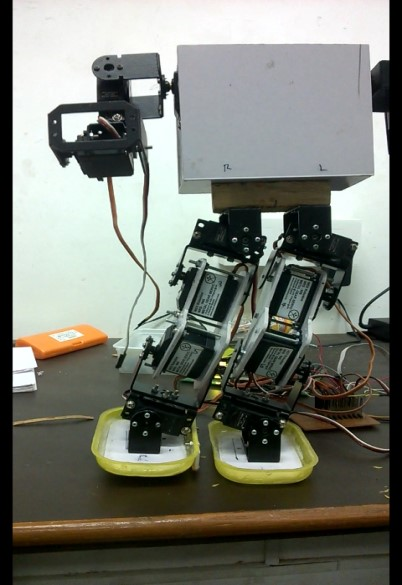
\includegraphics[width = 6cm,height= 7cm]{motion1_1.jpg}}
	\newline
	
	\caption{Basic swing}
	\label{fig:p2motion}
\end{figure}
\newline
\textbf{Calculation:} \\
Total height if the robot = $330 mm $.
Calculating the distance of CG from reference line using equation.\eqref{equ: Com} we get, \newline
$Xcom =152 mm $.\\
Distance of CG from the ground $=178mm$.\\
Angle $\beta = \tan^{-1} \frac{62}{178} =19.3 \degree $
\newpage
\flushleft  \textbf{Basic knee swing:}This motion can be described as balancing of robot on one leg where
the CG of robot is transferred completely on the balancing leg. The motion is little
different from basic swing for the fact that here the two additional servo are used for rising
the leg. The Figure \ref{fig:p2motion1} is a side view of the robot. In lifting the leg from ground angle
traversed by the lower hip servo should be equal to the angle traversed by the knee servo
but in opposite direction as shown in Fig \ref{fig:p2motion1} $\theta_{1}$ is equal to $\theta_{2}$.\\
\begin{figure}[h!]
	
	\centering
	\subfloat{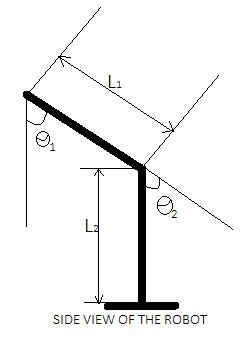
\includegraphics[width = 6cm,height= 7cm]{m2.jpg}} 
	\hspace{2cm}
	\subfloat{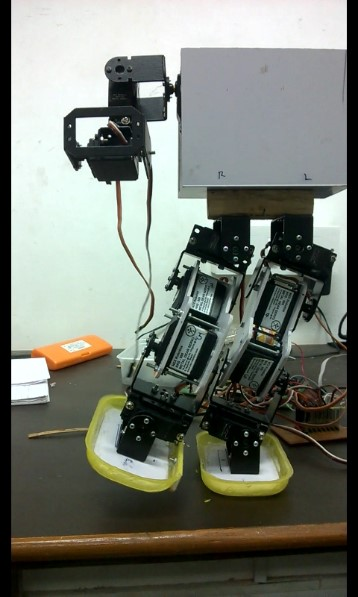
\includegraphics[width = 6cm,height= 7cm]{m2_1.jpg}}
	\newline
	
	\caption{Basic knee swing}
	\label{fig:p2motion1}
\end{figure}

$L_{1}$ = distance from lower hip servo to knee servo.\\
$L_{2}$ = distance from knee servo to foot.

\vspace{1cm}
\flushleft  \textbf{Walking:} walk is defined as movement by putting forward each foot in turn, not having
both feet off the ground at once. Every human has a specific unique walk, hence gait
means manner of walking. Moreover, every walk is realized with certain gait. Gait can
divided into four phases as shown in Fig \ref{fig:footprint}.\\
\begin{enumerate}
	\item Double Support Phase (DSP)\\
	This is the phase where both feet are fully supported with the floor
	\item Pre-Swing Phase\\
	In this phase the heel of the rear foot is lifting from the floor but the biped is still in
	double support phase due to the fact that the toes of this foot are still on the floor
	\item Single Support Phase\\
	The phase where only one foot is fully supported with the floor and the other foot
	swing forward
	\item Post-Swing Phase\\
	In this phase the toe of the front foot is declining towards the floor. The robot is in
	double support because the heel of this foot is contacting the floor.
\end{enumerate}
\newpage
\begin{figure}
	\centering
	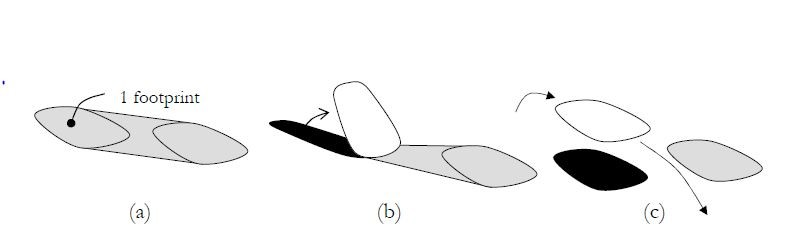
\includegraphics[width = 16cm,height= 8cm]{footprint}
	\caption{Shaded grey region is the support polygon \cite{zero}.a) double support phase
		b) Double support (pre swing phase) c) single support}
	\label{fig:footprint}
\end{figure}

We move from double support phase to single support phase with help of basic swing and
knee motion and then place the raised leg forward. While placing the raised leg forward
the lower hip servo and knee servo on the other leg should rotate in anti-clockwise and the
knee servo should move in clockwise direction till the raised leg reaches the ground. Then
CG is transferred form one leg to the other and then the leg from which the CG was
transferred to other leg is raised by motion of lower hip servo in anti-clockwise and knee
servo in clockwise direction till it comes in line with body when seen from side of the
robot and then the sequence is followed to keep the leg on the ground and shift the CG.
\vspace{3cm}

\subsection{Motion of the Phase 3 structure}
Similarly in this structure the motion is categorized in three phases which are
\begin{enumerate}
	\item Basic swing
	\item Basic knee swing
	\item Walking
\end{enumerate}
\newpage
\textbf{Basic swing:} The motion is similar as stated above but since the CG has changed the angle
to transverse by the servo during the swing motion will change and is calculated as below.
\begin{figure}[h!]
	
	\centering
	\subfloat{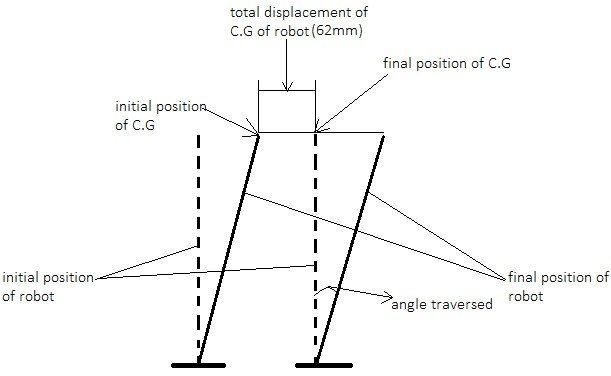
\includegraphics[width = 6cm,height= 7cm]{m3.jpg}} 
	\hspace{2cm}
	\subfloat{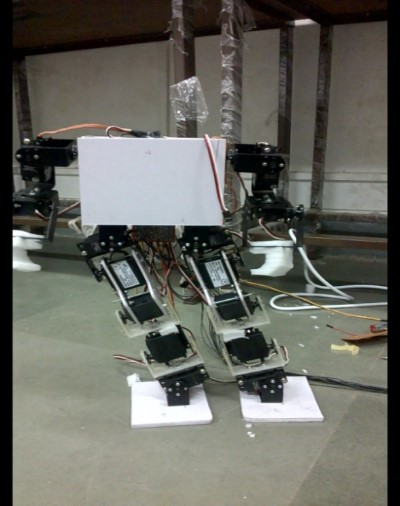
\includegraphics[width = 6cm,height= 7cm]{m3_1.jpg}}
	\newline
	
	\caption{Basic swing}
\end{figure}
\newline
\textbf{Calculation:} \\
Total height if the robot = $400 mm $.
Calculating the distance of CG from reference line using equation.\eqref{equ: Com} we get, \newline
$Xcom =159.184 mm $.\\
Distance of CG from the ground $= 400-159.184= 240.816 mm.$.\\
Angle $\beta = \tan^{-1} \frac{70}{240.816} =16.21 \degree $\\

\textbf{Basic knee swing:} As shown below in Fig \ref{fig:p3motion} the knee swing can be achieved by motion
of lower hip servo, upper ankle servo in same direction and rotated by same angle and
knee servo should rotate in opposite direction by an angle double of that of the hip and
upper ankle servo. From the Figure below we derive a relationship between angle as $\theta_{2} =
\theta_{1} + \theta_{3}$.
\begin{figure}[h!]
	
	\centering
	\subfloat{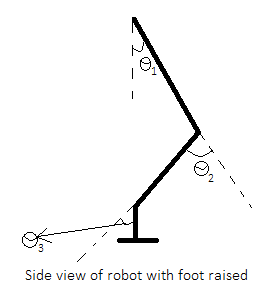
\includegraphics[width = 6cm,height= 7cm]{m4}} 
	\hspace{2cm}
	\subfloat{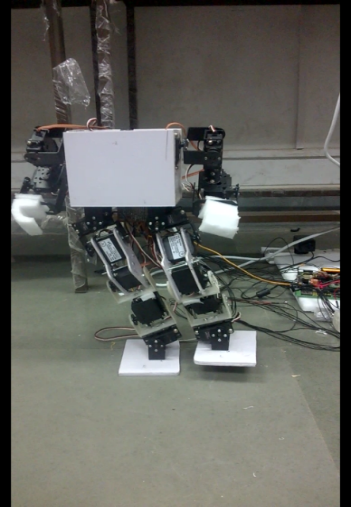
\includegraphics[width = 6cm,height= 7cm]{m4_1}}
	\newline
	
	\caption{Basic knee swing}
	\label{fig:p3motion}
\end{figure}
\newpage
\textbf{Walking:} We move from double support phase to single support phase with help basic
swing and knee motion and then place the raised leg forward. While placing the raised leg
forward the ankle servo of the other leg is rotated in clockwise motion when viewed from
side of the bot which pushes the bot forward and then CG is transferred form one leg to the
other, the leg from which the CG was transferred to other leg is raised by motion of lower
hip servo in anti-clockwise, knee servo in clockwise direction and upper ankle servo in
clockwise direction till it comes in line with body when seen from side of the robot and
sequence is followed again for the next step.


\section{Electronic Design}
All robots require a number of servo motors to provide actuation and sensors to sense the
environment around; these sensors and actuators are controlled using the processing unit.
In this project currently a single micro-controller is used which is ATMEGA640. This
micro-controller is used to control all the servo motors which are 16 in numbers and
corresponds to 16 degrees of freedom.\\
ATMEGA 640 Features:
\begin{itemize}
	\item High Performance, Low Power AVR® 8-Bit Micro-controller
	\item 64K Bytes of In-System Self-Programmable Flash
	\item 4K Bytes EEPROM
	\item 8K Bytes Internal SRAM
	\item Up to 64K Bytes Optional External Memory Space
	\item Two 8-bit Timer/Counters with Separate Prescaler and Compare Mode
	\item Four 16-bit Timer/Counter with Separate Prescaler, Compare- and Capture Mode
	\item Four 8-bit PWM Channels
	\item Twelve PWM Channels with Programmable Resolution from 2 to 16 Bits
	\item 16-channel, 10-bit ADC
	\item Interrupt and Wake-up on Pin Change
\end{itemize}
\begin{figure}[h!]
	\centering
	\subfloat{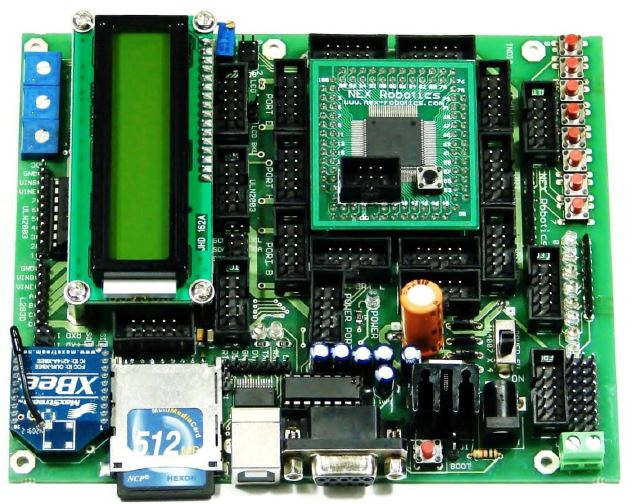
\includegraphics[width = 6cm,height= 4cm]{A640}}
	\caption{ATMEGA640 development board}
\end{figure}
\newpage
\subsection{Connections}
The IO pins of the microcontroller are used to drive the servo motors. We require to drive
16 servos hence we need 16 IO pins. Hence we use Port E pin 0 to 7 and Port B pin 0 to 7
of the microcontroller to drive these servos. Setting up the Ports to deliver required PWM
signals will be dealt in latter part of document.
The servos are powered by an external power supply to provide sufficient current and the
control pins are connected to the corresponding port pins of the microcontroller as shown
in figure below.
\begin{figure}[h!]
	\centering
	\subfloat{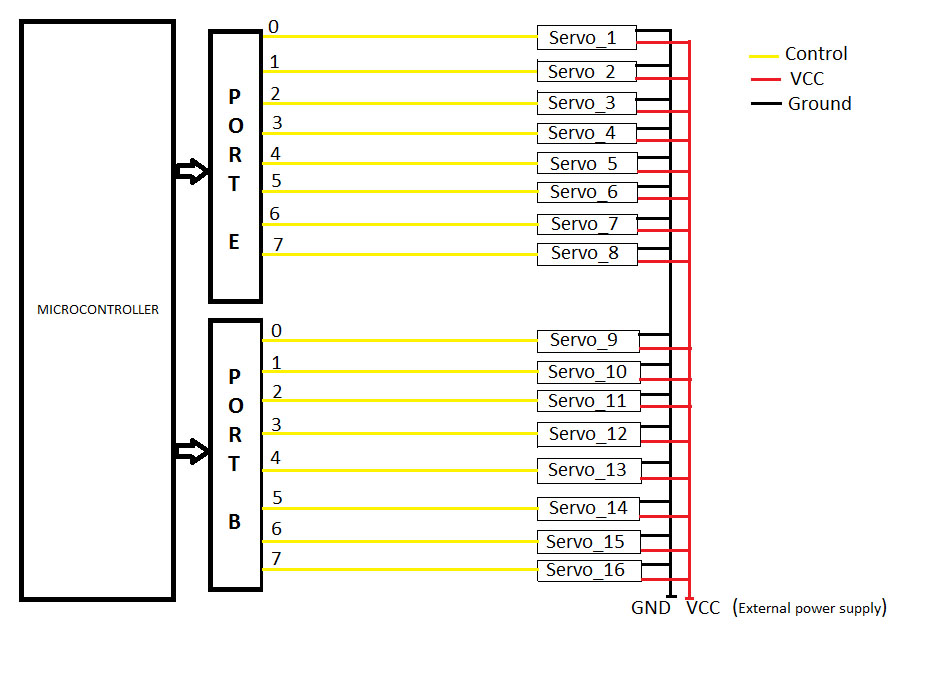
\includegraphics[width = 8cm,height= 6cm]{schematic_connections.jpg}}
	\caption{Schematic of servo pin connection with microcontroller port}
\end{figure}
Here our main emphasis will be on the timers of the microcontroller, since these timers are
used to generate PWM signals required for driving Servo motors. In ATMEGA640 there
are two 8 bit timers and four 16 bit timers. Here we will be using these 16 bit timers for
generating PWM signal of required frequency for driving the servo motors.
Servo motors are a type of electromechanical actuators that do not rotate continuously like
DC, AC or stepper motors, rather they are used to position and hold some object. They are
used where continuous rotation is not required as in the case of our Humanoid Robot
where there are restrictions on the movements of hand and leg joints. Here we use High
Torque RC Servo Motor with metal gears (NRS-995) weighted 77gms which can provide
torque of 15.5kgfcm @4.8V and 17kgfcm @6V. These are analog servos which basically
work with 50 Hz PWM signal i.e a pulse width of 20ms. The datasheet specifies that a TON
of 0.6ms is required for 0 degree rotation and 2.2ms for 180 degree rotation.\\
\subsection{PWM generation}
Basically there are two methods for generating the PWM signals which are required to
drive the Servo motors:\\
\textbf{Method 1:} Using the dedicated PWM output pins from the timer. Here in ATMEGA640
since we have four 16bit timers and each of these timers have three Output compare pins
we get 12 PWM channels. Hence using these analog pins attached to these timers can drive
up to maximum of 12 servo motors, which does not serve the purpose for us since we need
to drive 16 servo motors.\\
\textbf{Method 2:} This method uses one 16 bit timers to drive up to 24 servos on each timer. It
uses interrupts so no explicit refresh activity is required. The pulse width (20ms) required
for servo operation is divided into 8 pulses of 2.5ms each. And during this each pulse of
2.5ms 3 servo motors can be driven through 3 digital output pins. Hence we end up driving
up to 24 servo motors during the entire pulse width. This method also gives a better
resolution compared to the first method so we use this method to drive 16 servo motors.\\
Steps to interface and drive servo motors using second method:\\
\begin{enumerate}
\item The timers are initialized to a value get a pulse width of 2.5ms in 16bit Fast PWM
mode.
\item The output ports required to drive servo motors are initialized, here we require 2
Ports.
\item Now this pulse of 2.5ms is multiplied by 8 to get a pulse width of 20ms which is
50Hz.
\item Since the timer has three Output Compare Registers (A, B and C), during each pulse
of 2.5ms three servo motors can be set to the required angle.
\item Set of three servos each defined as set\_number which can take values from 0 to 7.
\item We see that there are 8 such pulses (set\_numbers) and each of these can drive 3
servos.
\item The servo control pins are SET at overflow of timer during the corresponding pulse
(set\_number) of 2.5ms and RESET when OCR matches the Timer value using
Interrupts to get the required T-ON pulse which corresponds to the input angle
required.
\end{enumerate}
\vspace{2cm}
Now, for e.g consider set\_number 0 and set\_number 1.\\
set\_number 0 has servos 2, 4 and 6\\
Consider an instance when set\_number is 0 the following events occur, these events are
captured using interrupts:\\
\begin{enumerate}
	\item Timer value equals the Output Compare Register (OCR) value, during this event
	the following decisions are taken:
	\begin{itemize}
	\item Check the set\_number and RESET servo pin of the corresponding
	set\_number (here 0)\\
	\textit{*This step is applicable to all the OCRs i.e A, B and C}
	\end{itemize}
	\item Overflow of the timer occurs, during this event the following decisions are
	taken:
	\begin{itemize}
		\item Timer is reset to initial value which is required to generate 2.5 ms pulse
		width.
		\item set\_number is incremented by 1. If set\_number is greater than 7 reset it to
		0.
		\item Now, check the set\_number and SET the servo pins (here servos 2, 4 and
		6) of the corresponding set\_number (here 0) and also update the OCR A,
		B and C with values of required angles for servos of this set\_number
		(here servos 2, 4 and 6).
	\end{itemize}
\end{enumerate}
\newpage
\begin{figure}[h!]
	\centering
	\subfloat{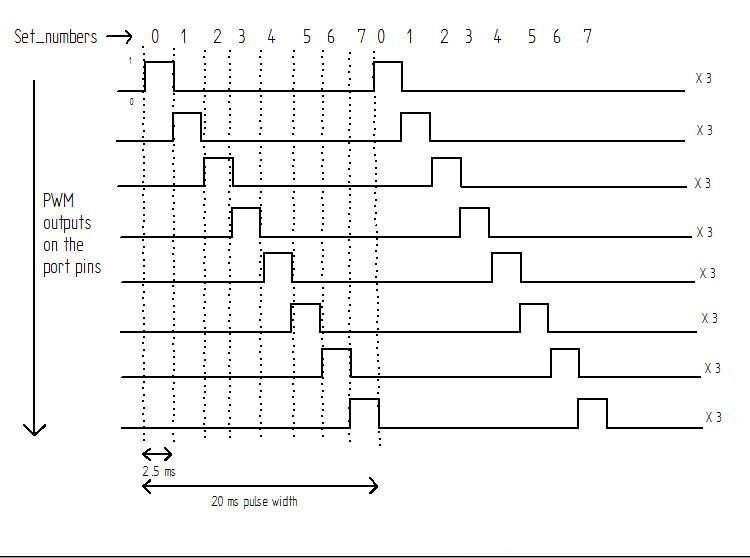
\includegraphics[width = 10cm,height= 7cm]{waveform.jpg}}
	\caption{PWM waveform generation using interrupts}
\end{figure}
Hence using this technique we can drive up to 24 servos at a time using a single timer.The
	Servo motors are provided with external power supply and the control pins are connected
	to the corresponding port pins.


\subsection{Power System}
In an autonomous system like Humanoid Robot the power required and efficiency of the
system becomes a crucial aspect. Since there are 16 servo motors each of which has a
rating of 4.8V and 500mA to provide the rated torque of 15.5kgcm and an On board
processor requiring at least 1A current.\\
Hence designing a compact power supply unit with sufficient current bank is an important
and challenging task also considering the weight of the power supply or batteries on the
robot.\\
Practically it was found that each servo with maximum torque drew a maximum current of
400 mA and a stall current of 100 mA.\\
So considering the working of all 16 servos simultaneously we require a power supply of
6V and $16 \times 400 = 6400 mA$.\\
Hence we can consider using a power supply of 6V and 5A to 7A power supply unit to
provide sufficient power to make sure the working of all the components in the worst case.
\underline{Block diagrams for Power Supply:}
\begin{center}
	\includegraphics[width = 10cm,height= 6cm]{ac.jpg}
	\newline
	
\end{center}
 \begin{center}
 	\includegraphics[width = 10cm,height= 6cm]{dc.jpg}
 \end{center}
 A Ni-MH battery rated 6V 5000mAh is used for the powering the servos externally.
 \begin{figure}[h!]
 	\centering
 	\subfloat{\includegraphics[width = 10cm,height= 7cm]{battery.jpg}}
 	\caption{Ni-MH battery 6V 5000mAh}
 \end{figure}
 
 \section{Problems faced with servo motors}
 \textbf{Servo Jitters:}\\
 Since there were 16 long signal cables going from microcontroller to the servo, there was
 interference between these signal cables. This caused distortions in the PWM signals of all
 other servos due to any one particular cable working at a time. This caused servo jitters
 which is the unwanted movement of servo motor.\\
 \textbf{Solution:}\\
 This problem can be resolved by using twisted pair cable for transmitting servo control
 signals. So we twisted the signal cable in groups of 5 and observed that the interference
 was reduced and obtained a less distorted PWM waveform.
 \newpage
 \begin{figure}[h!]
 	
 	\centering
 	\subfloat[Twisted signal wires]{\includegraphics[width = 7cm,height= 7cm]{wire}} 
 	\hspace{2cm}
 	\subfloat[Distortion reduced PWM signal]{\includegraphics[width = 7cm,height= 7cm]{wave}}
 	\newline
 	
 	\caption{Servo jitter}
 \end{figure}
 This problem aroused because we have been using a long signal wire for testing purpose
 from microcontroller to the robot. This problem will eliminated when the microcontroller
 is mounted on the robot which shortens the signal wire considerably and reduces the
 interference between this wires. This will result in a clean PWM signal which can drive the
 servo motors jitter free.\\
 
 \flushleft  \textbf{Inadequate Servo Torque:}\\
 The rated servo motor torque is given to be 17kgcm at 6V operating voltage. But this servo motors are not quite efficient in that case. And these motors are not suitable for a 16 DOFs humanoid robot since at one particular instance the whole body weight is taken by a single servo. Since the length of the robot has increased the effective torque of the servo motor decreases, for e.g if the length is 10cm then the torque is 1.7kg, this is very less for the existing design considering the fact that the height of the robot is 40cm.\\
 Hence in such case if we needed an angle of 10\degree than we had to give an angle more than that to get desired angle because the servo would not hold the weight as the entire bot weight sums to 1.82kg excluding the battery. And it is because of these servos the battery could not be mounted on the robot as it increase the overall weight.\\
 Even at its stationary lock positions these servos tend to move a little bit because of the joint of the plastic flaps and the metal gear. This causes a problem during the motion of the robot.\\ 
 These servo motors are suited for robotic arm grippers where the base is fixed and for bi-piped robot where weight is considerably less because it doesn't have the upper body.\\
    
\flushleft \textbf{Solution:}\\
These servo problem can be solved by replacing these servo motors by a much powerful digital servo motors. If not all the servos at least the servos which take most of the body weight like the Hip servos and the Ankle servos.
 \newpage
 
 \section{Future Work}
 \begin{itemize}
 	\item Making modules for different possible movements.
 	\item Interfacing gyros for auto stabilization of the robot.
 	\item Building a GUI for controlling the robot autonomously.
 	\item Interfacing camera along with a smart processor like raspberry pi or a beagle board for identifying objects
 	\item Interfacing various sensors like ultrasonic sensors for distance calculation,
 	accelerometer, Xbee for wireless communication. 
 	\item Interfacing with modules like Kinect to depict the human motion and many more.
 \end{itemize}
 
 \begin{thebibliography}{99}
 \bibitem{zero} Zero-moment point method for stable biped walking\\
DCT no.: 2009.072\\
Internship report\\
Eindhoven, July 2009.\\

\bibitem{real} Real Time Biped Walking Gait Pattern Generator for a Real Robot\\
Department of Computer Science and Technology,\\
University of Science and Technology of China,\\
Hefei, 230026, China\\

\bibitem{design} Design and Implementation of a Simplified Humanoid Robot with 8 DOF\\
Department of Electronics and Communication Engineering,\\ Hindustan Institute of
Technology and Science,\\ Hindustan University, Chennai, India\\

\bibitem{kin} Kinematics and Inverse Kinematics for the Humanoid Robot\\
Rowland O’Flahertyy, Peter Vieiray, Michael Greyy,\\
Paul Ohz, Aaron Bobicky, Magnus Egerstedty, and Mike Stilmany\\

\bibitem{kinematics} Kinematics and Dynamics of a New 16 DOF Humanoid Biped Robot with Active Toe Joint\\
Regular Paper\\
C. Hernández-Santos, E. Rodriguez-Leal1, R. Soto1 and J.L. Gordillo\\

\newpage
\bibitem{robotic} Robotics (12 of Addis Ababa Lectures): Forward Kinematics of Spatial Robots\\
\url{https://www.youtube.com/watch?v=NXWzk1toze4}\\

\bibitem{robotic1}Robotics (1/3 of INGOU Lectures): An Introduction and Kinematic Configuration\\
\url{https://www.youtube.com/watch?v=gNhK4VoV9P8}\\

\bibitem{robotics2}Robotics (2/3 of IGNOU Lectures): Kinematics--Denavit and Hartenberg Parameters\\
\url{https://www.youtube.com/watch?v=CnWTUsVle2A}\\

\bibitem{robotics3}Robotics (3/3 of IGNOU Lectures): Forward and Inverse Kinematic Analyses\\
\url{https://www.youtube.com/watch?v=duKD8cvtBTI}\\

\bibitem{roboticswalk}Robot Basic Walk Tutorial\\
\url{https://www.youtube.com/watch?v=Xhz6m6fu494}\\

 \end{thebibliography}

\end{document}


	